\documentclass[11pt,4paper]{report}
\usepackage[top=2.2cm,bottom=2cm]{geometry}
\usepackage[separate-uncertainty, exponent-product=\cdot, per-mode=symbol, binary-units=true]{siunitx}
\usepackage{graphicx}
\usepackage[italian]{babel}
\usepackage[utf8]{inputenc}
\usepackage{amsmath}
\usepackage{float}
\usepackage{circuitikz}
\usepackage{pgfplots}
\usepackage{epsfig}
\usepackage{subcaption}
\usepackage[colorlinks=true, allcolors=blue]{hyperref}
\usepackage[most]{tcolorbox}

\newcommand{\vcc}{$V_{cc}$}
\newcommand{\iic}{$\text{I}^2\text{C}$}

%Define environment for datasheets
\newcounter{datasheetcnt}
\renewcommand{\thedatasheetcnt}{\arabic{datasheetcnt}}
\newenvironment{datasheet}[2]{\refstepcounter{datasheetcnt}\par\bigskip\medskip \label{#2}
	\noindent \underline{\textsc{Datasheet~\thedatasheetcnt}}: \textbf{#1} \newline}{\medskip}

\title{Sistemi Digitali Integrati \\ \large Lezioni del Prof. Ruo Roch}
\author{Marco Andorno}


\begin{document}
\maketitle
\tableofcontents
\chapter{Memorie: RAM e ROM}
\section{Classificazione}
Una memoria è un oggetto in cui si possono mettere delle informazioni per poi ritrovarle. Una possibile tassonomia è la seguente:
\begin{itemize}
	\item Modalità di lettura e scrittura:
	\begin{itemize}
		\item Read-only (ROM): si possono solo leggere. In realtà, ad oggi non esistono memorie che si possano solo leggere ed il termine ROM sta quindi ad indicare una memoria in cui è più facile leggere che scrivere.
		\item Read-write (RAM): si possono leggere e scrivere. Si chiamano RAM perché le prime memorie read-write erano anche ad accesso casuale ed il termine è rimasto come sinonimo.
	\end{itemize}
	\item Modalità di accesso:
	\begin{itemize}
		\item Accesso casuale: i dati possono essere letti in ordine arbitrario (RAM, NOR flash).
		\item Accesso sequenziale: i dati possono essere letti solo in sequenze predefinite (NAND flash, HDD, FIFO, LIFO, nastri magnetici). Ancora oggi nei data center i backup sono effettuati su nastri magnetici perché costano poco e sono passivi.
	\end{itemize}
	\item Modalità per reperire l'informazione:
	\begin{itemize}
		\item Accesso per indirizzo: ogni oggetto memorizzato ha un indirizzo univoco con cui si può reperire.
		\item Accesso per contenuto: l'informazione non è organizzata in modo geografico, ma secondo etichette che ne identificano il contenuto.
	\end{itemize}
	\item Permanenza dell'informazione in assenza di alimentazione:
	\begin{itemize}
		\item Volatile: togliendo energia al sistema, l'informazione viene persa (memoria del PC).
		\item Non volatile: togliendo energia al sistema, l'informazione rimane comunque memorizzata.
	\end{itemize}
	\pagebreak
	\item Permanenza dell'informazione nel tempo:
	\begin{itemize}
		\item Statica: la memoria funziona anche a frequenza 0, l'informazione è mantenuta finché c'è alimentazione.
		\item Dinamica: l'informazione tende a svanire nel tempo, anche se l'alimentazione rimane e perciò serve un \emph{refresh} periodico per mantenerla (memoria del pc, CD/DVD riscrivibili a cambio di fase, in cui la probabilità di cambio di fase è funzione esponenziale della temperatura, o anche memorie flash, in cui il \emph{data retention} è circa 10 anni a \SI{25}{\celsius}). Questo pone dei problemi nell'archiviazione di dati storici.
	\end{itemize}
\end{itemize}

\section{RAM statica (SRAM)}
Innanzitutto il nome SRAM non è univoco: dal punto di vista storico, quando è nata la RAM statica, quella dinamica non esisteva e quindi la si è chiamata semplicemente RAM. La S è stata aggiunta solo in seguito per distinguere i due tipi, ma per evitare equivoci è preferibile riferirsi ad essa come ``RAM statica''.

\subsection{Struttura interna}
La RAM statica non è nient'altro che un array di latch in cui viene conservato il dato, realizzati in tecnologia CMOS con due inverter collegati in parallelo (figura \ref{fig:latch}). Le trans-caratteristiche di tali inverter sono mostrate in figura \ref{fig:trans}. Ognuno dei due inverter vuole imporre la sua equazione ed entrambi hanno ragione contemporaneamente, quindi si evidenziano tre punti di equilibrio distinti, che vanno analizzati dal punto di vista della stabilità. 
\begin{figure}[H]
	\centering
	\begin{circuitikz}
		\draw
		(1,0) node[not port, label={[centered,xshift=-4pt] {A}}] (not1) {}
		(1,-2) node[not port, rotate=180, label={[centered,xshift=4pt] {B}}] (not2) {}
		(not2.out) -- (-1,-2) to[short, label=$1$] (-1,0) -- (not1.in)
		(not1.out) -- (3,0) to[short, label=$2$] (3,-2) -- (not2.in)
		;
	\end{circuitikz}
	\caption{Cella base della SRAM}
	\label{fig:latch}
\end{figure}
\begin{figure}[hbtp]
	\centering
	% This file was created by matlab2tikz.
%
%The latest updates can be retrieved from
%  http://www.mathworks.com/matlabcentral/fileexchange/22022-matlab2tikz-matlab2tikz
%where you can also make suggestions and rate matlab2tikz.
%
\definecolor{mycolor1}{rgb}{0.00000,0.44700,0.74100}%
\definecolor{mycolor2}{rgb}{0.85000,0.32500,0.09800}%
\definecolor{mycolor3}{rgb}{0.92900,0.69400,0.12500}%
%
\begin{tikzpicture}[scale=0.8]

\begin{axis}[%
axis lines = left,
width=4.521in,
height=3.566in,
at={(0.758in,0.481in)},
scale only axis,
xmin=0,
xmax=6,
xtick={0,5},
xticklabels={{0},{$\text{V}_{\text{cc}}$}},
ymin=0,
ymax=6,
ytick={0,5},
yticklabels={{0},{$\text{V}_{\text{cc}}$}},
axis background/.style={fill=white},
legend style={legend cell align=left, align=left, draw=white!15!black}
]
\addplot [color=black]
  table[row sep=crcr]{%
0	5\\
0.0252525252525253	5\\
0.0505050505050505	4.99999999999993\\
0.0757575757575758	4.99999999999822\\
0.101010101010101	4.99999999998225\\
0.126262626262626	4.99999999989418\\
0.151515151515152	4.99999999954498\\
0.176767676767677	4.99999999843826\\
0.202020202020202	4.9999999954549\\
0.227272727272727	4.99999998833824\\
0.252525252525253	4.99999997290907\\
0.277777777777778	4.99999994192818\\
0.303030303030303	4.99999988351394\\
0.328282828282828	4.99999977901092\\
0.353535353535354	4.99999960019495\\
0.378787878787879	4.99999930568898\\
0.404040404040404	4.99999883645322\\
0.429292929292929	4.99999811020211\\
0.454545454545455	4.99999701458969\\
0.47979797979798	4.99999539899405\\
0.505050505050505	4.99999306472075\\
0.53030303030303	4.99998975343391\\
0.555555555555556	4.999985133613\\
0.580808080808081	4.9999787848222\\
0.606060606060606	4.99997017956864\\
0.631313131313131	4.99995866251436\\
0.656565656565657	4.99994342679654\\
0.681818181818182	4.99992348719902\\
0.707070707070707	4.99989764990776\\
0.732323232323232	4.99986447857149\\
0.757575757575758	4.99982225637817\\
0.782828282828283	4.99976894384695\\
0.808080808080808	4.99970213202414\\
0.833333333333333	4.9996189907612\\
0.858585858585859	4.99951621174136\\
0.883838383838384	4.99938994591094\\
0.909090909090909	4.99923573496034\\
0.934343434343434	4.99904843648875\\
0.95959595959596	4.99882214247577\\
0.984848484848485	4.99855009067214\\
1.01010101010101	4.99822456851089\\
1.03535353535354	4.99783680912934\\
1.06060606060606	4.99737687908134\\
1.08585858585859	4.99683355730837\\
1.11111111111111	4.99619420492703\\
1.13636363636364	4.99544462537967\\
1.16161616161616	4.99456891448395\\
1.18686868686869	4.99354929990609\\
1.21212121212121	4.99236596957182\\
1.23737373737374	4.99099688851798\\
1.26262626262626	4.98941760367687\\
1.28787878787879	4.98760103607452\\
1.31313131313131	4.98551725991305\\
1.33838383838384	4.98313326799646\\
1.36363636363636	4.98041272294835\\
1.38888888888889	4.97731569365876\\
1.41414141414141	4.97379837638698\\
1.43939393939394	4.96981279993571\\
1.46464646464646	4.96530651430141\\
1.48989898989899	4.96022226219451\\
1.51515151515152	4.95449763281238\\
1.54040404040404	4.94806469723702\\
1.56565656565657	4.94084962481836\\
1.59090909090909	4.93277227989336\\
1.61616161616162	4.92374579817996\\
1.64141414141414	4.91367614217428\\
1.66666666666667	4.9024616348681\\
1.69191919191919	4.88999247109335\\
1.71717171717172	4.87615020578875\\
1.74242424242424	4.86080721847341\\
1.76767676767677	4.84382615320074\\
1.79292929292929	4.82505933325564\\
1.81818181818182	4.80434814984651\\
1.84343434343434	4.78152242403306\\
1.86868686868687	4.7563997411198\\
1.89393939393939	4.72878475673423\\
1.91919191919192	4.69846847379773\\
1.94444444444444	4.66522748958646\\
1.96969696969697	4.62882321206833\\
1.9949494949495	4.58900104469148\\
2.02020202020202	4.54548953878858\\
2.04545454545455	4.49799951275044\\
2.07070707070707	4.44622313711144\\
2.0959595959596	4.3898329846785\\
2.12121212121212	4.32848104482411\\
2.14646464646465	4.26179770105335\\
2.17171717171717	4.18939067094363\\
2.1969696969697	4.11084390754519\\
2.22222222222222	4.02571646131926\\
2.24747474747475	3.93354130167999\\
2.27272727272727	3.83382409719531\\
2.2979797979798	3.72604195349098\\
2.32323232323232	3.6096421078911\\
2.34848484848485	3.48404057981743\\
2.37373737373737	3.34862077595912\\
2.3989898989899	3.20273204921323\\
2.42424242424242	3.04568821038572\\
2.44949494949495	2.87676599163167\\
2.47474747474747	2.69520346060236\\
2.5	2.50019838425623\\
2.5	2.49980161574377\\
2.52525252525253	2.30479653939764\\
2.55050505050505	2.12323400836833\\
2.57575757575758	1.95431178961428\\
2.6010101010101	1.79726795078677\\
2.62626262626263	1.65137922404088\\
2.65151515151515	1.51595942018257\\
2.67676767676768	1.3903578921089\\
2.7020202020202	1.27395804650902\\
2.72727272727273	1.16617590280469\\
2.75252525252525	1.06645869832001\\
2.77777777777778	0.974283538680735\\
2.8030303030303	0.889156092454809\\
2.82828282828283	0.810609329056375\\
2.85353535353535	0.738202298946654\\
2.87878787878788	0.671518955175887\\
2.9040404040404	0.610167015321499\\
2.92929292929293	0.553776862888562\\
2.95454545454545	0.502000487249565\\
2.97979797979798	0.454510461211418\\
3.00505050505051	0.410998955308519\\
3.03030303030303	0.371176787931671\\
3.05555555555556	0.334772510413542\\
3.08080808080808	0.30153152620227\\
3.10606060606061	0.271215243265771\\
3.13131313131313	0.243600258880198\\
3.15656565656566	0.218477575966943\\
3.18181818181818	0.195651850153493\\
3.20707070707071	0.174940666744359\\
3.23232323232323	0.156173846799257\\
3.25757575757576	0.139192781526589\\
3.28282828282828	0.123849794211246\\
3.30808080808081	0.110007528906654\\
3.33333333333333	0.0975383651319015\\
3.35858585858586	0.0863238578257227\\
3.38383838383838	0.0762542018200358\\
3.40909090909091	0.0672277201066436\\
3.43434343434343	0.0591503751816397\\
3.45959595959596	0.0519353027629828\\
3.48484848484848	0.0455023671876238\\
3.51010101010101	0.0397777378054942\\
3.53535353535354	0.0346934856985873\\
3.56060606060606	0.0301872000642867\\
3.58585858585859	0.0262016236130204\\
3.61111111111111	0.0226843063412405\\
3.63636363636364	0.019587277051652\\
3.66161616161616	0.0168667320035385\\
3.68686868686869	0.0144827400869544\\
3.71212121212121	0.0123989639254758\\
3.73737373737374	0.0105823963231272\\
3.76262626262626	0.00900311148202204\\
3.78787878787879	0.00763403042818078\\
3.81313131313131	0.00645070009390967\\
3.83838383838384	0.0054310855160504\\
3.86363636363636	0.00455537462033081\\
3.88888888888889	0.00380579507297162\\
3.91414141414141	0.00316644269162646\\
3.93939393939394	0.00262312091865581\\
3.96464646464646	0.00216319087065844\\
3.98989898989899	0.0017754314891071\\
4.01515151515152	0.00144990932785809\\
4.04040404040404	0.00117785752422762\\
4.06565656565657	0.000951563511250772\\
4.09090909090909	0.00076426503966208\\
4.11616161616162	0.000610054089059598\\
4.14141414141414	0.000483788258637679\\
4.16666666666667	0.00038100923879649\\
4.19191919191919	0.000297867975859515\\
4.21717171717172	0.00023105615305328\\
4.24242424242424	0.000177743621826656\\
4.26767676767677	0.000135521428510107\\
4.29292929292929	0.000102350092238361\\
4.31818181818182	7.65128009830156e-05\\
4.34343434343434	5.65732034646656e-05\\
4.36868686868687	4.13374856372155e-05\\
4.39393939393939	2.98204313600811e-05\\
4.41919191919192	2.12151777970719e-05\\
4.44444444444444	1.48663870037954e-05\\
4.46969696969697	1.02465660884993e-05\\
4.49494949494949	6.93527925432461e-06\\
4.52020202020202	4.60100595401412e-06\\
4.54545454545454	2.98541031118e-06\\
4.57070707070707	1.88979788530344e-06\\
4.5959595959596	1.16354678070123e-06\\
4.62121212121212	6.94311022760375e-07\\
4.64646464646465	3.99805047806097e-07\\
4.67171717171717	2.2098907603385e-07\\
4.6969696969697	1.16486060000318e-07\\
4.72222222222222	5.80718242335756e-08\\
4.74747474747475	2.70909345872056e-08\\
4.77272727272727	1.16617590280468e-08\\
4.7979797979798	4.54510461211418e-09\\
4.82323232323232	1.56173846799258e-09\\
4.84848484848485	4.55023671876235e-10\\
4.87373737373737	1.05823963231272e-10\\
4.8989898989899	1.77543148910713e-11\\
4.92424242424242	1.77743621826654e-12\\
4.94949494949495	6.93527925432473e-14\\
4.97474747474747	2.70909345872041e-16\\
5	0\\
};
%\addlegendentry{data1}

\addplot [color=black]
  table[row sep=crcr]{%
5	0\\
5	0.0252525252525253\\
4.99999999999993	0.0505050505050505\\
4.99999999999822	0.0757575757575758\\
4.99999999998225	0.101010101010101\\
4.99999999989418	0.126262626262626\\
4.99999999954498	0.151515151515152\\
4.99999999843826	0.176767676767677\\
4.9999999954549	0.202020202020202\\
4.99999998833824	0.227272727272727\\
4.99999997290907	0.252525252525253\\
4.99999994192818	0.277777777777778\\
4.99999988351394	0.303030303030303\\
4.99999977901092	0.328282828282828\\
4.99999960019495	0.353535353535354\\
4.99999930568898	0.378787878787879\\
4.99999883645322	0.404040404040404\\
4.99999811020211	0.429292929292929\\
4.99999701458969	0.454545454545455\\
4.99999539899405	0.47979797979798\\
4.99999306472075	0.505050505050505\\
4.99998975343391	0.53030303030303\\
4.999985133613	0.555555555555556\\
4.9999787848222	0.580808080808081\\
4.99997017956864	0.606060606060606\\
4.99995866251436	0.631313131313131\\
4.99994342679654	0.656565656565657\\
4.99992348719902	0.681818181818182\\
4.99989764990776	0.707070707070707\\
4.99986447857149	0.732323232323232\\
4.99982225637817	0.757575757575758\\
4.99976894384695	0.782828282828283\\
4.99970213202414	0.808080808080808\\
4.9996189907612	0.833333333333333\\
4.99951621174136	0.858585858585859\\
4.99938994591094	0.883838383838384\\
4.99923573496034	0.909090909090909\\
4.99904843648875	0.934343434343434\\
4.99882214247577	0.95959595959596\\
4.99855009067214	0.984848484848485\\
4.99822456851089	1.01010101010101\\
4.99783680912934	1.03535353535354\\
4.99737687908134	1.06060606060606\\
4.99683355730837	1.08585858585859\\
4.99619420492703	1.11111111111111\\
4.99544462537967	1.13636363636364\\
4.99456891448395	1.16161616161616\\
4.99354929990609	1.18686868686869\\
4.99236596957182	1.21212121212121\\
4.99099688851798	1.23737373737374\\
4.98941760367687	1.26262626262626\\
4.98760103607452	1.28787878787879\\
4.98551725991305	1.31313131313131\\
4.98313326799646	1.33838383838384\\
4.98041272294835	1.36363636363636\\
4.97731569365876	1.38888888888889\\
4.97379837638698	1.41414141414141\\
4.96981279993571	1.43939393939394\\
4.96530651430141	1.46464646464646\\
4.96022226219451	1.48989898989899\\
4.95449763281238	1.51515151515152\\
4.94806469723702	1.54040404040404\\
4.94084962481836	1.56565656565657\\
4.93277227989336	1.59090909090909\\
4.92374579817996	1.61616161616162\\
4.91367614217428	1.64141414141414\\
4.9024616348681	1.66666666666667\\
4.88999247109335	1.69191919191919\\
4.87615020578875	1.71717171717172\\
4.86080721847341	1.74242424242424\\
4.84382615320074	1.76767676767677\\
4.82505933325564	1.79292929292929\\
4.80434814984651	1.81818181818182\\
4.78152242403306	1.84343434343434\\
4.7563997411198	1.86868686868687\\
4.72878475673423	1.89393939393939\\
4.69846847379773	1.91919191919192\\
4.66522748958646	1.94444444444444\\
4.62882321206833	1.96969696969697\\
4.58900104469148	1.9949494949495\\
4.54548953878858	2.02020202020202\\
4.49799951275044	2.04545454545455\\
4.44622313711144	2.07070707070707\\
4.3898329846785	2.0959595959596\\
4.32848104482411	2.12121212121212\\
4.26179770105335	2.14646464646465\\
4.18939067094363	2.17171717171717\\
4.11084390754519	2.1969696969697\\
4.02571646131926	2.22222222222222\\
3.93354130167999	2.24747474747475\\
3.83382409719531	2.27272727272727\\
3.72604195349098	2.2979797979798\\
3.6096421078911	2.32323232323232\\
3.48404057981743	2.34848484848485\\
3.34862077595912	2.37373737373737\\
3.20273204921323	2.3989898989899\\
3.04568821038572	2.42424242424242\\
2.87676599163167	2.44949494949495\\
2.69520346060236	2.47474747474747\\
2.50019838425623	2.5\\
2.49980161574377	2.5\\
2.30479653939764	2.52525252525253\\
2.12323400836833	2.55050505050505\\
1.95431178961428	2.57575757575758\\
1.79726795078677	2.6010101010101\\
1.65137922404088	2.62626262626263\\
1.51595942018257	2.65151515151515\\
1.3903578921089	2.67676767676768\\
1.27395804650902	2.7020202020202\\
1.16617590280469	2.72727272727273\\
1.06645869832001	2.75252525252525\\
0.974283538680735	2.77777777777778\\
0.889156092454809	2.8030303030303\\
0.810609329056375	2.82828282828283\\
0.738202298946654	2.85353535353535\\
0.671518955175887	2.87878787878788\\
0.610167015321499	2.9040404040404\\
0.553776862888562	2.92929292929293\\
0.502000487249565	2.95454545454545\\
0.454510461211418	2.97979797979798\\
0.410998955308519	3.00505050505051\\
0.371176787931671	3.03030303030303\\
0.334772510413542	3.05555555555556\\
0.30153152620227	3.08080808080808\\
0.271215243265771	3.10606060606061\\
0.243600258880198	3.13131313131313\\
0.218477575966943	3.15656565656566\\
0.195651850153493	3.18181818181818\\
0.174940666744359	3.20707070707071\\
0.156173846799257	3.23232323232323\\
0.139192781526589	3.25757575757576\\
0.123849794211246	3.28282828282828\\
0.110007528906654	3.30808080808081\\
0.0975383651319015	3.33333333333333\\
0.0863238578257227	3.35858585858586\\
0.0762542018200358	3.38383838383838\\
0.0672277201066436	3.40909090909091\\
0.0591503751816397	3.43434343434343\\
0.0519353027629828	3.45959595959596\\
0.0455023671876238	3.48484848484848\\
0.0397777378054942	3.51010101010101\\
0.0346934856985873	3.53535353535354\\
0.0301872000642867	3.56060606060606\\
0.0262016236130204	3.58585858585859\\
0.0226843063412405	3.61111111111111\\
0.019587277051652	3.63636363636364\\
0.0168667320035385	3.66161616161616\\
0.0144827400869544	3.68686868686869\\
0.0123989639254758	3.71212121212121\\
0.0105823963231272	3.73737373737374\\
0.00900311148202204	3.76262626262626\\
0.00763403042818078	3.78787878787879\\
0.00645070009390967	3.81313131313131\\
0.0054310855160504	3.83838383838384\\
0.00455537462033081	3.86363636363636\\
0.00380579507297162	3.88888888888889\\
0.00316644269162646	3.91414141414141\\
0.00262312091865581	3.93939393939394\\
0.00216319087065844	3.96464646464646\\
0.0017754314891071	3.98989898989899\\
0.00144990932785809	4.01515151515152\\
0.00117785752422762	4.04040404040404\\
0.000951563511250772	4.06565656565657\\
0.00076426503966208	4.09090909090909\\
0.000610054089059598	4.11616161616162\\
0.000483788258637679	4.14141414141414\\
0.00038100923879649	4.16666666666667\\
0.000297867975859515	4.19191919191919\\
0.00023105615305328	4.21717171717172\\
0.000177743621826656	4.24242424242424\\
0.000135521428510107	4.26767676767677\\
0.000102350092238361	4.29292929292929\\
7.65128009830156e-05	4.31818181818182\\
5.65732034646656e-05	4.34343434343434\\
4.13374856372155e-05	4.36868686868687\\
2.98204313600811e-05	4.39393939393939\\
2.12151777970719e-05	4.41919191919192\\
1.48663870037954e-05	4.44444444444444\\
1.02465660884993e-05	4.46969696969697\\
6.93527925432461e-06	4.49494949494949\\
4.60100595401412e-06	4.52020202020202\\
2.98541031118e-06	4.54545454545454\\
1.88979788530344e-06	4.57070707070707\\
1.16354678070123e-06	4.5959595959596\\
6.94311022760375e-07	4.62121212121212\\
3.99805047806097e-07	4.64646464646465\\
2.2098907603385e-07	4.67171717171717\\
1.16486060000318e-07	4.6969696969697\\
5.80718242335756e-08	4.72222222222222\\
2.70909345872056e-08	4.74747474747475\\
1.16617590280468e-08	4.77272727272727\\
4.54510461211418e-09	4.7979797979798\\
1.56173846799258e-09	4.82323232323232\\
4.55023671876235e-10	4.84848484848485\\
1.05823963231272e-10	4.87373737373737\\
1.77543148910713e-11	4.8989898989899\\
1.77743621826654e-12	4.92424242424242\\
6.93527925432473e-14	4.94949494949495\\
2.70909345872041e-16	4.97474747474747\\
0	5\\
};
%\addlegendentry{data2}

\addplot [color=mycolor1, draw=none, mark=*, mark options={solid, fill=black, black}]
  table[row sep=crcr]{%
0	5\\
};
%\addlegendentry{data3}

\addplot [color=mycolor2, draw=none, mark=*, mark options={solid, fill=black, black}]
  table[row sep=crcr]{%
2.5	2.5\\
};
%\addlegendentry{data4}

\addplot [color=mycolor3, draw=none, mark=*, mark options={solid, fill=black, black}]
  table[row sep=crcr]{%
5	0\\
};
%\addlegendentry{data5}

\end{axis}
\end{tikzpicture}%
	\caption{Trans-caratteristica degli inverter con i tre punti di equilibrio evidenziati}
	\label{fig:trans}
\end{figure}

Supponiamo di essere nel punto centrale e che una fonte di disturbo dall'esterno alzi il potenziale del nodo 1: l'uscita di A scende e quindi B si trova in ingresso una tensione più bassa e la sua uscita sale. Ma l'uscita di B è l'ingresso di A, quindi il processo si ripete ed in breve tempo ci si porta in un altro punto di equilibrio. Il punto centrale è quindi instabile. 

In altri termini, si può vedere il sistema come un anello in retroazione: nel punto centrale il guadagno d'anello è maggiore di 1 perché la caratteristica è più ripida di \SI{45}{\degree} e quindi una perturbazione viene amplificata ad ogni giro. Negli altri due punti, invece, la perturbazione viene attenuata perché non ha praticamente effetto sull'uscita dal momento che la caratteristica è piatta, quindi essi sono punti di equilibrio stabili.

Con due stati stabili quindi questo oggetto è adatto a memorizzare un bit di informazione ed è anche robusto dal punto di vista del rumore.

\subsection{Lettura e scrittura}
Per poter leggere e scrivere, la cella base viene collegata a due linee dette \textbf{bitline} tramite due pass transistor, i cui gate sono collegati insieme ad una terza linea chiamata \textbf{wordline}.
\begin{itemize}
	\item \textbf{Lettura}. Se la wordline è a 0 logico i due pass transistor sono spenti, il latch è isolato e continua a conservare l'informazione. Applicando \vcc\ alla wordline, i transistor si accendono e sia l'informazione, sia il suo negato, vengono trasferiti sulle bitline. 
	\item \textbf{Scrittura}. Il valore da scrivere viene caricato sulle bitline e la wordline viene selezionata. Dal momento che i driver delle bitline sono molto più grandi dei transistor della cella, il latch cambia stato e memorizza il bit.
\end{itemize}

\begin{figure}[H]
	\centering
	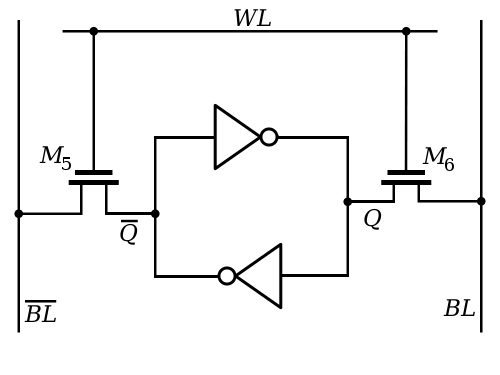
\includegraphics[width=0.6\linewidth]{memorie/SRAM_Cell_Inverter_Loop.png}
	\caption{Cella base della SRAM con bitline e wordline}
	\label{fig:SRAMcell}
\end{figure}

Questo blocco base si può replicare in verticale per aumentare il numero di parole (righe), o in orizzontale per aumentare il numero di bit per parola (colonne). Così le celle possono essere migliaia, ma ogni NMOS ha delle capacità parassite nell'ordine dei \si{\femto\farad} tra drain e substrato o tra source e substrato, dovute alle giunzioni polarizzate inversamente (perché il substrato è al potenziale di \SI{0}{\volt}). Quindi la capacità totale di ogni linea può diventare facilmente dell'ordine dei \si{\pico\farad}. 

Effettuando una lettura, quindi, una delle due bitline deve essere sempre caricata a \vcc: ipotizzando che il pass transitor chiuso si comporti da resistenza, il risultato è una risposta esponenziale del primo ordine, con una costante di tempo $\tau = RC$. Inoltre, ogni latch ha dimensioni ridotte per poter ottimizzare l'area, quindi la sua resistenza di canale elevata va a sommarsi a tale costante di tempo, che può diventare dell'ordine del \si{\micro\second}, ovvero molto lunga. Ancor peggio, dal momento che la capacità della bitline è molto più grande di quella del latch, potrebbe avvenire un fenomeno, detto \textbf{bit flip}, per cui la linea impone un valore al latch, operando a tutti gli effetti come in scrittura e quindi cambiando il valore del bit memorizzato. Questo è possibile perché ogni punto di equilibrio è stabile solo per perturbazioni piccole: se tali disturbi sono troppo elevati, il sistema può cambiare stato.

La soluzione consiste nel \textbf{precaricare} le grandi capacità delle bitline ad una tensione innocua, pari a \vcc/2: attivando poi la wordline, una linea andrà verso 0, l'altra verso 1 (figura \ref{fig:precharge}). Il problema della lentezza non è risolto, se non in parte, mentre il bit flip sì. Tuttavia, ora, basta fare la differenza tra il valore \vcc/2 di partenza delle bitline, con quello assunto poco dopo tramite dei comparatori con isteresi, chiamati \textbf{sense amplifier}. 
\begin{figure}[hbtp]
	\centering
	% This file was created by matlab2tikz.
%
%The latest updates can be retrieved from
%  http://www.mathworks.com/matlabcentral/fileexchange/22022-matlab2tikz-matlab2tikz
%where you can also make suggestions and rate matlab2tikz.
%
\begin{tikzpicture}[scale=0.9]

\begin{axis}[%
axis lines = left,
width=4.521in,
height=3.566in,
at={(0.758in,0.481in)},
scale only axis,
xmin=0,
xmax=5,
xtick={0,1,2,3,4,5},
xticklabels={{0},{$\tau$},{$\text{2}\tau$},{$\text{3}\tau$},{$\text{4}\tau$},{$\text{5}\tau$}},
ymin=0,
ymax=1,
ytick={0,0.5,1},
yticklabels={{0},{$\text{V}_{\text{cc}}\text{/2}$},{$\text{V}_{\text{cc}}$}},
axis background/.style={fill=white},
legend style={legend cell align=left, align=left, draw=white!15!black}
]
\addplot [color=black]
  table[row sep=crcr]{%
0	0.5\\
0.0505050505050505	0.475374563448467\\
0.101010101010101	0.451961951147641\\
0.151515151515152	0.429702430444255\\
0.202020202020202	0.408539210570366\\
0.252525252525253	0.388418297752938\\
0.303030303030303	0.369288357459399\\
0.353535353535354	0.351100583427727\\
0.404040404040404	0.333808573146915\\
0.454545454545455	0.317368209470141\\
0.505050505050505	0.30173754805858\\
0.555555555555556	0.286876710368716\\
0.606060606060606	0.272747781910122\\
0.656565656565657	0.259314715514124\\
0.707070707070707	0.24654323936658\\
0.757575757575758	0.234400769570118\\
0.808080808080808	0.222856327012759\\
0.858585858585859	0.211880458330838\\
0.909090909090909	0.201445160764567\\
0.95959595959596	0.191523810714524\\
1.01010101010101	0.182091095816807\\
1.06060606060606	0.173122950363536\\
1.11111111111111	0.164596493903953\\
1.16161616161616	0.15648997286948\\
1.21212121212121	0.148782705073783\\
1.26262626262626	0.141455026946263\\
1.31313131313131	0.134488243364342\\
1.36363636363636	0.12786457995655\\
1.41414141414141	0.121567137754733\\
1.46464646464646	0.115579850079672\\
1.51515151515152	0.109887441550127\\
1.56565656565657	0.104475389110721\\
1.61616161616162	0.0993298849792354\\
1.66666666666667	0.0944378014187809\\
1.71717171717172	0.089786657244972\\
1.76767676767677	0.0853645859826514\\
1.81818181818182	0.0811603055909241\\
1.86868686868687	0.0771630896792594\\
1.91919191919192	0.0733627401412257\\
1.96969696969697	0.069749561136037\\
2.02020202020202	0.0663143343515315\\
2.07070707070707	0.06304829548547\\
2.12121212121212	0.0599431118851505\\
2.17171717171717	0.056990861288292\\
2.22222222222222	0.0541840116109479\\
2.27272727272727	0.0515154017308821\\
2.32323232323232	0.048978223217381\\
2.37373737373737	0.0465660029608881\\
2.42424242424242	0.0442725866581444\\
2.47474747474747	0.0420921231106996\\
2.52525252525253	0.0400190492967359\\
2.57575757575758	0.0380480761781171\\
2.62626262626263	0.0361741752064528\\
2.67676767676768	0.0343925654937517\\
2.72727272727273	0.0326987016149301\\
2.77777777777778	0.0310882620110582\\
2.82828282828283	0.0295571379637567\\
2.87878787878788	0.0281014231126139\\
2.92929292929293	0.026717403488879\\
2.97979797979798	0.0254015480400048\\
3.03030303030303	0.0241504996208651\\
3.08080808080808	0.0229610664286622\\
3.13131313131313	0.0218302138596731\\
3.18181818181818	0.0207550567670575\\
3.23232323232323	0.0197328520999763\\
3.28282828282828	0.0187609919052388\\
3.33333333333333	0.0178369966736262\\
3.38383838383838	0.0169585090139136\\
3.43434343434343	0.0161232876384522\\
3.48484848484848	0.0153292016449665\\
3.53535353535354	0.014574225079979\\
3.58585858585859	0.0138564317699894\\
3.63636363636364	0.0131739904072244\\
3.68686868686869	0.0125251598774172\\
3.73737373737374	0.0119082848176989\\
3.78787878787879	0.0113217913932672\\
3.83838383838384	0.010764183282058\\
3.88888888888889	0.0102340378571752\\
3.93939393939394	0.00973000255733953\\
3.98989898989899	0.00925079143609549\\
4.04040404040404	0.00879518188097343\\
4.09090909090909	0.00836201149423522\\
4.14141414141414	0.00795017512724627\\
4.19191919191919	0.0075586220609071\\
4.24242424242424	0.00718635332495134\\
4.29292929292929	0.00683241914927036\\
4.34343434343434	0.00649591654076269\\
4.39393939393939	0.00617598697952548\\
4.44444444444444	0.00587181422851068\\
4.49494949494949	0.00558262225105753\\
4.54545454545455	0.00530767323098834\\
4.5959595959596	0.00504626569021639\\
4.64646464646465	0.00479773269906319\\
4.6969696969697	0.0045614401747192\\
4.74747474747475	0.00433678526350688\\
4.7979797979798	0.00412319480281865\\
4.84848484848485	0.00392012385880581\\
4.8989898989899	0.00372705433608746\\
4.94949494949495	0.00354349365593259\\
5	0.00336897349954273\\
};
\addlegendentry{data1}

\addplot [color=black]
  table[row sep=crcr]{%
0	0.5\\
0.0505050505050505	0.524625436551533\\
0.101010101010101	0.548038048852359\\
0.151515151515152	0.570297569555745\\
0.202020202020202	0.591460789429634\\
0.252525252525253	0.611581702247062\\
0.303030303030303	0.630711642540601\\
0.353535353535354	0.648899416572273\\
0.404040404040404	0.666191426853085\\
0.454545454545455	0.682631790529859\\
0.505050505050505	0.69826245194142\\
0.555555555555556	0.713123289631284\\
0.606060606060606	0.727252218089878\\
0.656565656565657	0.740685284485876\\
0.707070707070707	0.75345676063342\\
0.757575757575758	0.765599230429882\\
0.808080808080808	0.777143672987241\\
0.858585858585859	0.788119541669162\\
0.909090909090909	0.798554839235433\\
0.95959595959596	0.808476189285476\\
1.01010101010101	0.817908904183193\\
1.06060606060606	0.826877049636464\\
1.11111111111111	0.835403506096047\\
1.16161616161616	0.84351002713052\\
1.21212121212121	0.851217294926217\\
1.26262626262626	0.858544973053737\\
1.31313131313131	0.865511756635658\\
1.36363636363636	0.87213542004345\\
1.41414141414141	0.878432862245267\\
1.46464646464646	0.884420149920328\\
1.51515151515152	0.890112558449873\\
1.56565656565657	0.895524610889279\\
1.61616161616162	0.900670115020765\\
1.66666666666667	0.905562198581219\\
1.71717171717172	0.910213342755028\\
1.76767676767677	0.914635414017349\\
1.81818181818182	0.918839694409076\\
1.86868686868687	0.922836910320741\\
1.91919191919192	0.926637259858774\\
1.96969696969697	0.930250438863963\\
2.02020202020202	0.933685665648468\\
2.07070707070707	0.93695170451453\\
2.12121212121212	0.94005688811485\\
2.17171717171717	0.943009138711708\\
2.22222222222222	0.945815988389052\\
2.27272727272727	0.948484598269118\\
2.32323232323232	0.951021776782619\\
2.37373737373737	0.953433997039112\\
2.42424242424242	0.955727413341856\\
2.47474747474747	0.9579078768893\\
2.52525252525253	0.959980950703264\\
2.57575757575758	0.961951923821883\\
2.62626262626263	0.963825824793547\\
2.67676767676768	0.965607434506248\\
2.72727272727273	0.96730129838507\\
2.77777777777778	0.968911737988942\\
2.82828282828283	0.970442862036243\\
2.87878787878788	0.971898576887386\\
2.92929292929293	0.973282596511121\\
2.97979797979798	0.974598451959995\\
3.03030303030303	0.975849500379135\\
3.08080808080808	0.977038933571338\\
3.13131313131313	0.978169786140327\\
3.18181818181818	0.979244943232942\\
3.23232323232323	0.980267147900024\\
3.28282828282828	0.981239008094761\\
3.33333333333333	0.982163003326374\\
3.38383838383838	0.983041490986086\\
3.43434343434343	0.983876712361548\\
3.48484848484848	0.984670798355033\\
3.53535353535354	0.985425774920021\\
3.58585858585859	0.986143568230011\\
3.63636363636364	0.986826009592776\\
3.68686868686869	0.987474840122583\\
3.73737373737374	0.988091715182301\\
3.78787878787879	0.988678208606733\\
3.83838383838384	0.989235816717942\\
3.88888888888889	0.989765962142825\\
3.93939393939394	0.99026999744266\\
3.98989898989899	0.990749208563904\\
4.04040404040404	0.991204818119027\\
4.09090909090909	0.991637988505765\\
4.14141414141414	0.992049824872754\\
4.19191919191919	0.992441377939093\\
4.24242424242424	0.992813646675049\\
4.29292929292929	0.99316758085073\\
4.34343434343434	0.993504083459237\\
4.39393939393939	0.993824013020475\\
4.44444444444444	0.994128185771489\\
4.49494949494949	0.994417377748942\\
4.54545454545455	0.994692326769012\\
4.5959595959596	0.994953734309784\\
4.64646464646465	0.995202267300937\\
4.6969696969697	0.995438559825281\\
4.74747474747475	0.995663214736493\\
4.7979797979798	0.995876805197181\\
4.84848484848485	0.996079876141194\\
4.8989898989899	0.996272945663913\\
4.94949494949495	0.996456506344067\\
5	0.996631026500457\\
};
\addlegendentry{data2}

\addplot [color=black, dashed]
  table[row sep=crcr]{%
0	0.5\\
5	0.5\\
};
\addlegendentry{data3}

\addplot [color=black, dashed]
  table[row sep=crcr]{%
0	1\\
5	1\\
};
\addlegendentry{data4}
\legend{}
\end{axis}
\end{tikzpicture}%
	\caption{Risposta esponenziale con la precarica}
	\label{fig:precharge}
\end{figure}


Così facendo, le RAM statiche sono ad oggi i dispositivi con il più basso tempo d'accesso, nell'ordine del \si{\nano\second}. Per questo sono utilizzate quando serve un consumo statico basso, o una velocità di lettura molto elevata.

\subsection{Interfaccia esterna}
Per ottimizzare l'utilizzo dell'area, si vorrebbe realizzare un array di memoria all'incirca quadrato, ma spesso il numero di righe è molto superiore al numero di colonne, quindi bisogna disporre le celle diversamente. Ad esempio, supponiamo di voler realizzare un array con 32768 word da 16 bit, ovvero da \SI{64}{\kilo\byte}. Per renderlo quanto più quadrato possibile, scegliamo di suddividerlo in 512 colonne e 1024 righe. Sapendo che non si attiva mai più di una wordline alla volta, in ingresso al chip si può mettere un decoder da 10 bit. Quindi, dei 512 bit in uscita se ne selezionano soltanto 16, ovvero la lunghezza della word, perciò si mette un multiplexer con 5 bit di selezione. Così facendo, il numero totale di bit di selezione è 15, che è proprio il numero necessario per indirizzare 32768 word.

In generale, se $R$ è il numero di righe, $C$ il numero di colonne e $W$ la lunghezza di una word, il decoder ha in ingresso $\log_2{R}$ bit che costituiscono il \textbf{bus indirizzi}, mentre il multiplexer necessita di $\log_2{(C/W)}$ bit di selezione, dove quindi i $W$ bit in uscita costituiscono il \textbf{bus dati} (figura \ref{fig:sram_array}).
\begin{figure}[hbtp]
	\centering
	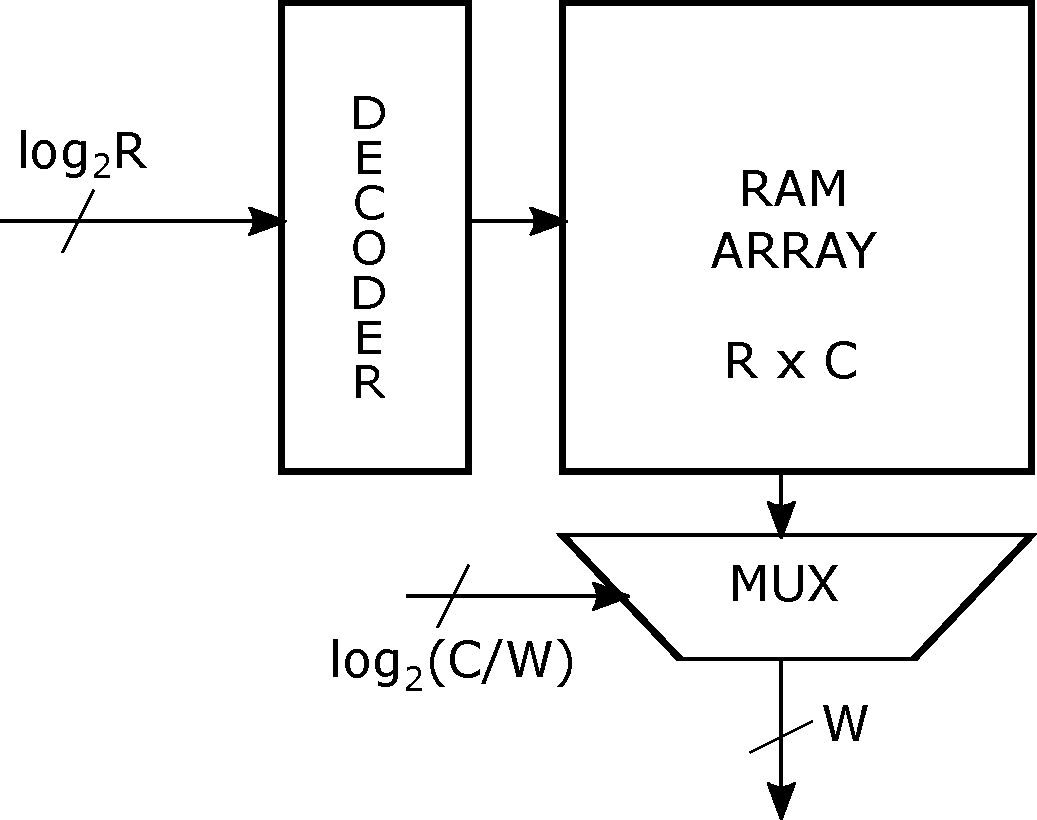
\includegraphics[width=0.4\linewidth]{memorie/sram_array.pdf}
	\caption{Interfaccia di un array di SRAM}
	\label{fig:sram_array}
\end{figure}


\subsubsection{Segnali di controllo}
In quanto oggetto nato negli anni '70, l'interfacciamento della RAM statica è completamente asincrono e, per mantenere la compatibilità all'indietro, i segnali di controllo sono rimasti gli stessi fino ad oggi:
\begin{itemize}
	\item \textbf{Chip Select}, Chip Enable o Enable ($\overline{CS}$, $\overline{CE}$ o $\overline{E}$): tipicamente attivo basso, serve per dire alla RAM che le si vuole parlare. Utile nel caso in cui ci siano più chip di RAM nel sistema, retaggio di quando le capacità delle memorie erano molto piccole e quindi si usava mettere molti chip. Oggi, con lo scaling tecnologico, spesso e volentieri basta un unico chip della capacità desiderata, ma il segnale è comunque utilizzato, ad esempio, per far entrare la RAM in modalità a basso consumo quando non è utilizzata.
	\item \textbf{Write enable} ($\overline{WE}$, $\overline{W}$, o $R/\overline{W}$): segnale attivo basso, vale 1 quando si vuole leggere e 0 quando si vuole scrivere.
	\item \textbf{Output Enable} ($\overline{OE}$ o $\overline{G}$): attivo basso, abilita le uscite della memoria, ovvero i buffer tri-state del bus dati bidirezionale. Si usa quando si hanno più RAM sullo stesso bus per eliminare eventuali conflitti.
\end{itemize}
Questi tre segnali ci sono sempre, ma magari insieme ad altri o modificati. Così si riescono a fare le operazioni fondamentali di lettura e scrittura.

\pagebreak

\subsection{Timing diagram}
\begin{figure}[hbtp]
	\centering
	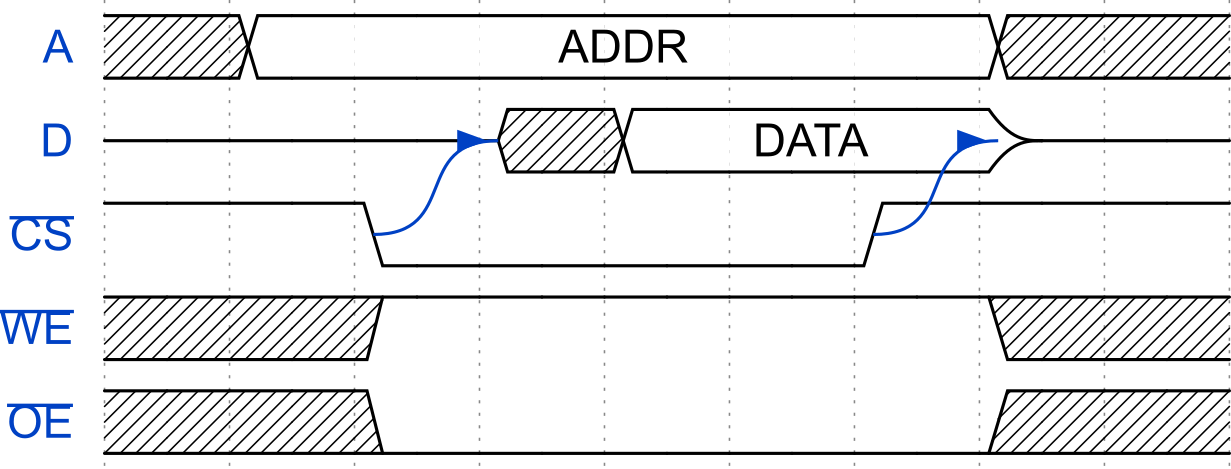
\includegraphics{memorie/sram_read.png}
	\caption{Timing di una SRAM in lettura}
	\label{fig:sram_read}
\end{figure}
Per leggere, ad un certo punto si mette l'indirizzo valido sul bus indirizzi ed il segnale $\overline{WE}$ viene posto a 1 logico. Il segnale $\overline{OE}$ viene asserito affinché le uscite siano abilitate e forniscano il dato. Finché il $\overline{CS}$ rimane a 1, lo stato degli altri segnali è irrilevante, perché la RAM è muta. 

Il bus dati è in alta impedenza finché la RAM non è abilitata, poi esce da questo stato una volta che $\overline{CS}$ viene asserito, ma il valore non è ancora corretto: bisogna attendere il tempo necessario per la lettura dall'array prima che il dato sia valido.

Per concludere la lettura, si toglie il $\overline{CS}$ e i dati tornano in alta impedenza. Quindi anche gli altri segnali di controllo possono essere disattivati.

In alternativa, si può abilitare $\overline{OE}$ solo quando i dati in uscita sono validi, in modo da risparmiare transizioni sul bus e quindi potenza. Tuttavia, bisogna essere in grado di capire quando i dati sono stabili, il che può complicare il circuito di controllo.

\begin{datasheet}{BSI BS62LV1600 Very Low Power CMOS SRAM 2M X 8 bit}{}
Il modello è del 2006, ma è ancora esistente tutt'oggi perché le SRAM sono apprezzate per la semplicità dei segnali di controllo che permette di limitare i costi di progetto.

L'array è $4096 \times 4096$ e lo schema a blocchi è del tutto simile a quello presentato prima. Ci sono due chip enable, spesso in questi casi sono messi in AND.

Il fatto che sia dichiarata come \emph{very low power} è del tutto indicativo: dipende dalla fonte di alimentazione, da quanto frequentemente viene letta o scritta ecc. Il vero risparmio energetico vi è quando il chip select è disattivato e la memoria va in power down.

È comune per le SRAM avere un ampio range di tensioni di alimentazione, il che torna comodo quando il sistema non ha una tensione di alimentazione costante, come nel caso di dispositivi alimentati a batterie al litio. Inoltre aumenta la flessibilità in quanto si possono utilizzare sistemi sia TTL che CMOS, ad esempio.

Per leggere o scrivere la memoria necessita di una tensione tra \SIrange{2.4}{5.5}{\volt}, ma i dati vengono conservati con tensioni fino a \SI{1.5}{\volt}. Un tipico esempio è una memoria tampone in cui si simula una memoria non volatile con una piccola batteria che mantenga la tensione minima. Quando si torna all'alimentazione normale, esiste un tempo da attendere prima che la memoria sia disponibile (figura \ref{fig:sram_data_ret}).
\begin{figure}[H]
	\centering
	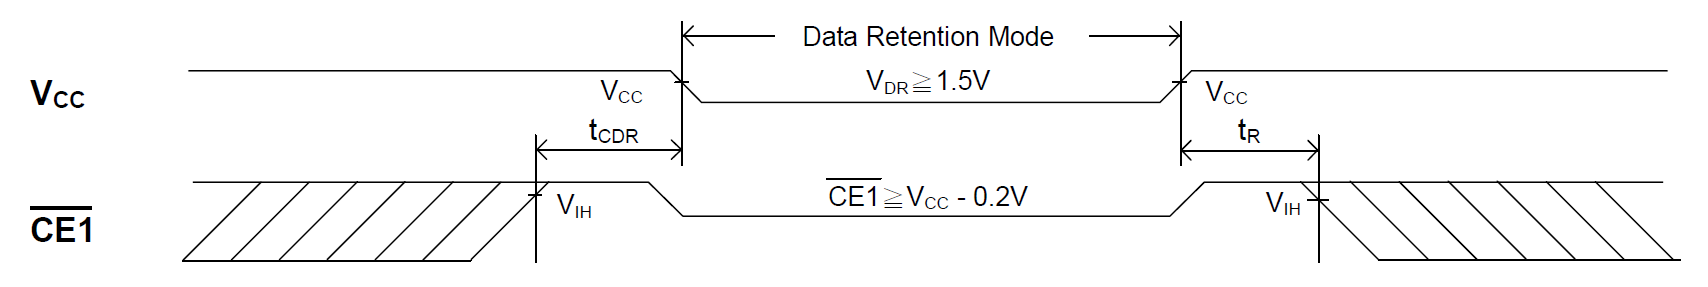
\includegraphics[width=\linewidth]{memorie/sram_data_retention.png}
	\caption{Timing per la modalità data retention}
	\label{fig:sram_data_ret}
\end{figure}

Se un dispositivo supera gli absolute maximum rating va subito buttato, perché anche se continuasse a funzionare dopo, non sarebbe più affidabile. 

Significativo è il dato riguardante la massima tensione negativa sopportabile dal chip, in quanto nei circuiti digitali le piste sulla scheda sono delle linee di trasmissione e quindi c'è il rischio di riflessioni.

Il dato sulla capacità dei piedini è utile per stimare il consumo e la velocità della transizione dei segnali.

L'entità della corrente di leakage è importante nel caso serva mettere una resistenza di pull-up sulle uscite tri-state, in modo da far sì che la caduta su tale resistenza sia trascurabile rispetto a quella del livello logico 1.

In riferimento alla figura \ref{fig:sram_read_cycle}, si noti che $D_{OUT}$ esce dall'alta impedenza ed inizia a commutare non appena sono passati tutti i tempi: $t_{OLZ}$, $t_{CLZ1}$ e $t_{CLZ2}$. Viceversa, il dato torna in alta impedenza quando è trascorso almeno uno tra gli intervalli di tempo $t_{OHZ}$, $t_{CHZ1}$ o $t_{CHZ2}$.
\begin{figure}[H]
	\centering
	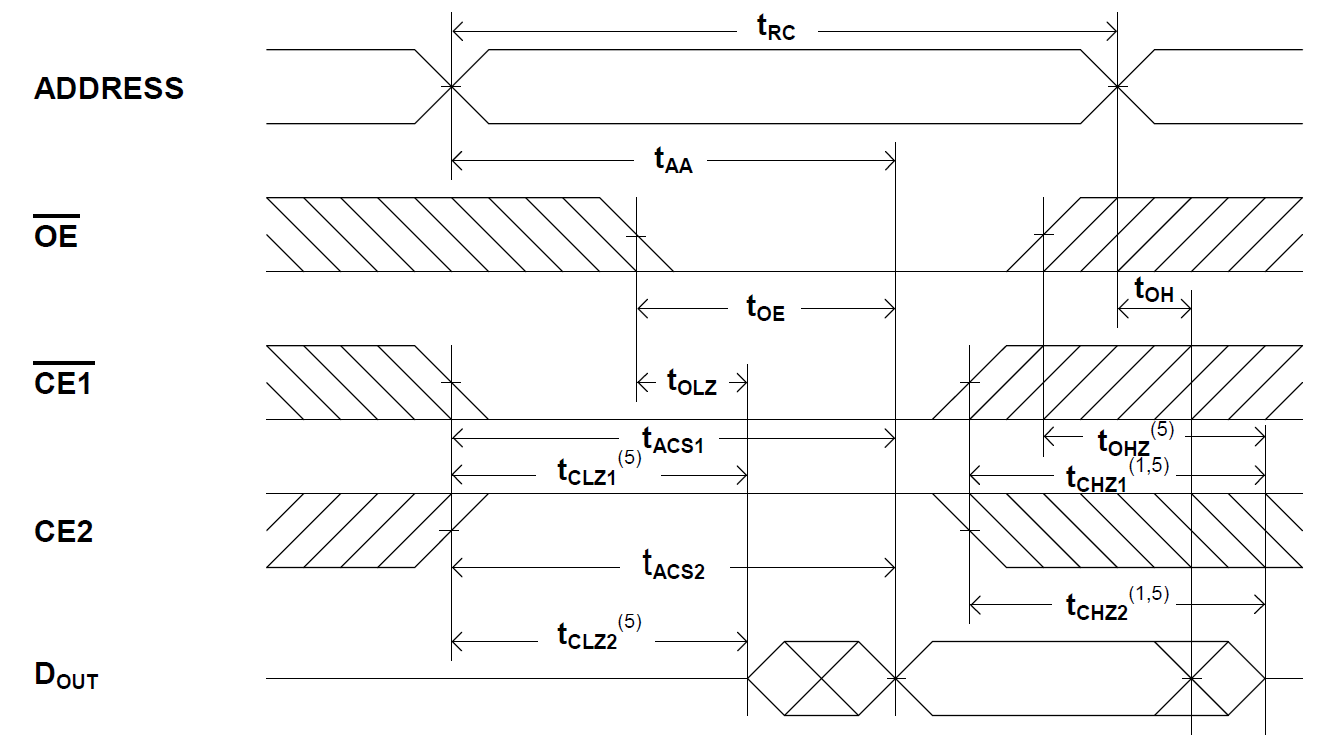
\includegraphics[width=\linewidth]{memorie/sram_read_cycle.png}
	\caption{Timing per il ciclo di lettura}
	\label{fig:sram_read_cycle}
\end{figure}
Ci sono due segnali che controllano la scrittura: $\overline{CS}$ e $\overline{WE}$. La RAM legge il dato quando uno di questi due viene disattivato.
\end{datasheet}

\subsection{SRAM sincrone (SSRAM)}
Le SRAM asincrone si comportano come un blocco di logica combinatoria in lettura e come un latch in scrittura, in cui il segnale di enable è il primo fronte di salita tra chip select o write enable. Il problema è che la generazione di tali segnali di controllo andrebbe fatta con una macchina asincrona, che è scomoda da fare. Inoltre, non c'è un'indicazione di quando il dato è valido, ma bisogna leggere i tempi di ritardo dal datasheet. Invece realizzare macchine sincrone è molto più comodo.

Non solo, tra il bus indirizzi e il dato in uscita c'è un ritardo di tipo combinatorio che in teoria lo scaling tecnologico dovrebbe permettere di ridurre. Con lo scaling, infatti, le dimensioni dei transistor diminuiscono, si riducono le capacità da pilotare e quindi la frequenza massima aumenta. Tuttavia, ciò funziona solo con le logiche ordinarie: in una memoria, mentre il decoder e il multiplexer scalano e diventano più veloci, nell'array i transistor più piccoli si utilizzano per aumentare la densità dei bit di memoria e quindi grosso modo la capacità totale delle bitline e wordline rimane invariata. 

Ciò ha dei risvolti anche sul mondo dei microprocessori. Negli anni si è passati da frequenze di pochi \si{\mega\hertz} fino a qualche \si{\giga\hertz} e poi basta. Questo è dovuto da un lato al fatto che anche aumentando la densità dei transistor, la velocità è limitata dal consumo di potenza che genera problemi di dissipazione man mano che l'area totale diminuisce. Dall'altro però, un microprocessore non lavora da solo, ma lo fa con delle memorie che, non riuscendo a salire di frequenza come i processori, non generano un grande interesse a spingere sempre più verso velocità maggiori.

Il percorso combinatorio può, però, essere diviso e fatto diventare sequenziale tramite la tecnica del \textbf{pipelining}: 
\begin{itemize}
	\item Dapprima si possono inserire registri sugli ingressi e sulle uscite. In questo modo, invece di avere ritardi puramente combinatori e variabili da segnale a segnale, si sa precisamente che il dato arriverà un ritardo $t_{CK \to Q}$ dopo il fronte. La massima frequenza di clock sarà limitata dal percorso critico tra l'ingresso del decoder e l'uscita del multiplexer, più  $t_{CK \to Q}$ del registro in ingresso e  $t_{SU}$ di quello in uscita.
	\item Quindi, si aggiungono registri anche dopo il decoder e prima del multiplexer: la frequenza massima diventa più elevata perché il percorso critico si è ridotto. Ragionevolmente esso sarà determinato dal tempo di attraversamento dell'array di memoria, in cui non si possono inserire ulteriori stadi di pipe.
\end{itemize}
In questo modo la SRAM è diventata sincrona: aumenta il throughput grazie alla frequenza maggiore, ma la latenza rimane invariata (3 colpi di clock nell'esempio). 

\begin{datasheet}{Samsung K7P80xx11B 256Kx36(x18) Synchronous Pipelined SRAM}{}
Le SSRAM non solo molto utilizzate oramai, ma sono utili per comprendere meglio poi le SDRAM. La memoria è piuttosto piccola perché, riducendo la dimensione dell'array, aumenta la velocità massima. 

Il parallelismo strano a 18 o 36 bit, serve in ambito telecom per fare delle FIFO o dei buffer con dei bit aggiuntivi di correzione automatica degli errori (ECC).

Ci sono due registri diversi per gli indirizzi di lettura e scrittura, dal momento che lettura e scrittura possono avere timing diversi. 

Nella RAM statica i segnali sono tutti degli strobe, mentre qua sono tutti campionati solo sul fronte del clock.

Il clock è \textbf{differenziale}: è composto da due segnali in controfase, in modo che il punto di riferimento temporale sia l'incrocio ta i due fronti. Questo rende tale riferimento indipendente dai tempi di salita e discesa.

Esistono quattro segnali aggiuntivi di write enable per scrivere byte singoli all'interno della parola intera.

Dal momento che, se i tempi di salita e discesa sono inferiori al tempo di propagazione sulla linea, le piste vanno considerate come linee di trasmissione, esiste la possibilità di regolare l'impedenza di uscita dei driver, tramite il pin ZQ.

Ci sono anche i 4 pin necessari per il protocollo di test JTAG.

Dal momento che questa è una memoria per alte prestazioni, anche il consumo di potenza è importante.

In figura \ref{fig:ssram_timing} è riportato un timing misto di letture e scritture. Si nota che dal momento in cui si dà il primo indirizzo, passano due colpi di clock prima di avere il dato pronto in uscita, ovvero la latenza è di due colpi di clock. Tuttavia, dando i successivi indirizzi senza aspettare il dato precedente, fa sì che, una volta che i dati iniziano ad uscire, lo facciano di continuo, evidenziando il throughput. 

Inoltre il primo dato diventa disponibile quando la memoria non è selezionata, ma è irrilevante perché si riferisce all'indirizzo dato in precedenza.

In scrittura, viene prima dato l'indirizzo e solo al colpo di clock dopo viene dato il dato.
\begin{figure}[hbtp]
	\centering
	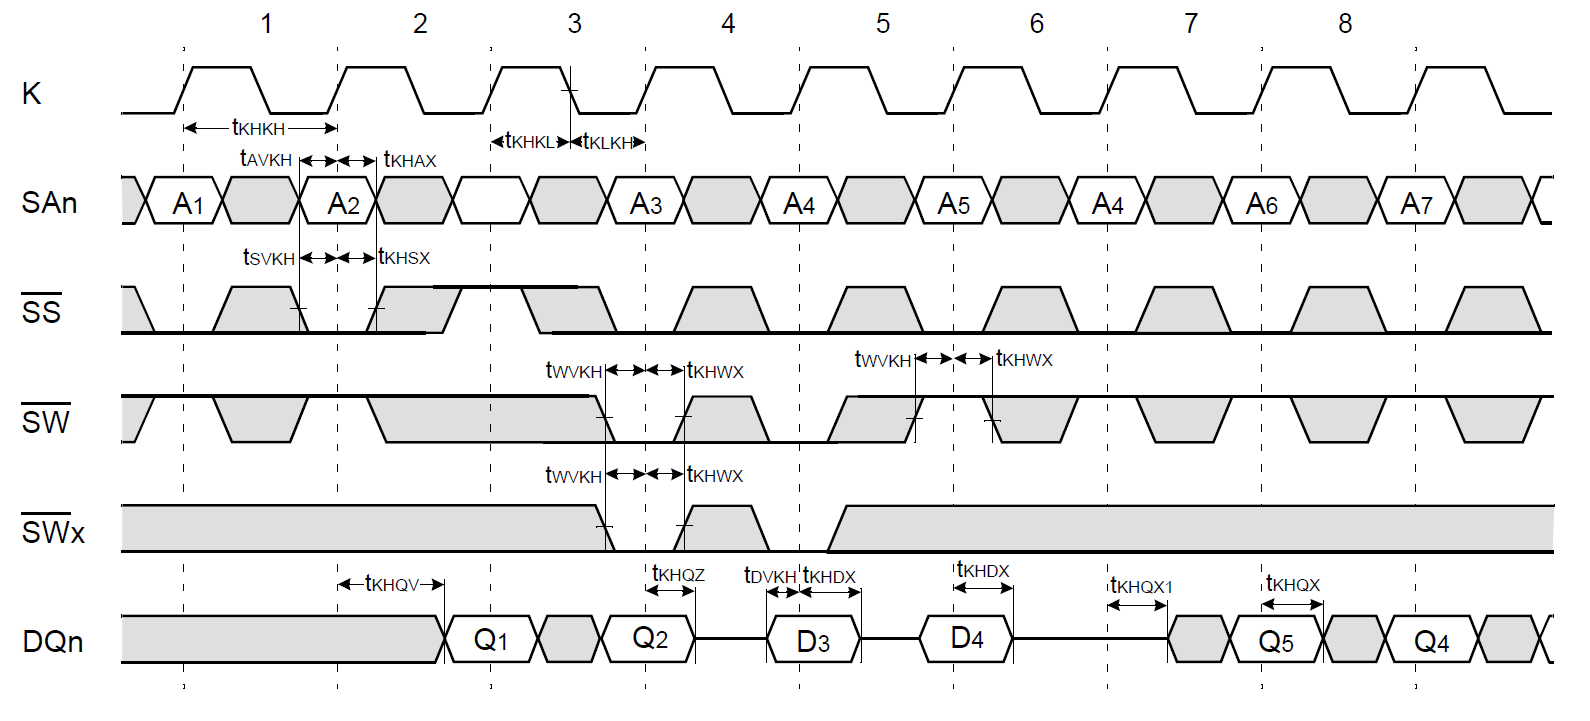
\includegraphics[width=\linewidth]{memorie/ssram_timing}
	\caption{Timing di una SSRAM}
	\label{fig:ssram_timing}
\end{figure}
\end{datasheet}

\section{RAM dinamica (DRAM)}
La RAM dinamica è una memoria volatile ad accesso casuale che però non può funzionare a frequenza 0, anche con l'alimentazione accesa l'informazione pian piano svanisce. Nasce poco dopo la RAM statica, in tecnologia MOS perché la cella base consiste solo di un condensatore, che si può realizzare facilmente con la capacità tra gate e substrato di un NMOS, con drain e source cortocircuitati a massa. Il fatto che tale capacità non sia lineare è irrilevante perché è di interesse solo quando è scarica o carica a $V_{cc}$. Il guadagno in termini di area rispetto alla SRAM è notevole, in quanto la cella base richiede solo 1 MOS, invece di 6.

\subsection{Struttura interna}
Un pass transistor connette il condensatore alla wordline ed una volta chiuso la carica si trasferisce nella bitline (figura \ref{fig:dram_cell}). Non c'è la bitline negata perché la cella base non è formata da inverter.
\begin{figure}[H]
	\centering
	% XCircuit output "dram_cell.tex" for LaTeX input from dram_cell.eps
\def\putbox#1#2#3#4{\makebox[0in][l]{\makebox[#1][l]{}\raisebox{\baselineskip}[0in][0in]{\raisebox{#2}[0in][0in]{\scalebox{#3}{#4}}}}}
\def\rightbox#1{\makebox[0in][r]{#1}}
\def\centbox#1{\makebox[0in]{#1}}
\def\topbox#1{\raisebox{-0.60\baselineskip}[0in][0in]{#1}}
\def\midbox#1{\raisebox{-0.20\baselineskip}[0in][0in]{#1}}
\begin{center}
   \scalebox{0.8}{
   \normalsize
   \parbox{2.8125in}{
   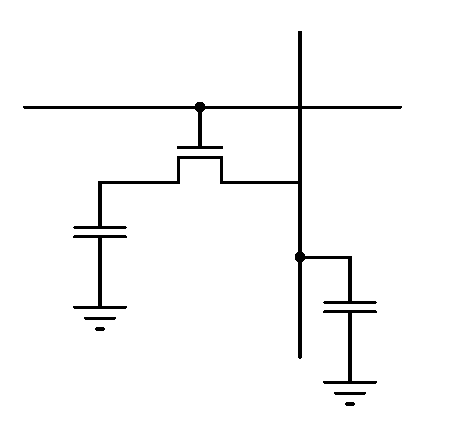
\includegraphics[scale=1]{memorie/dram_cell.eps}\\
   % translate x=640 y=348 scale 0.38
   \putbox{1.97in}{2.45in}{1.20}{$BL$}%
   \putbox{0.14in}{2.20in}{1.20}{$WL$}%
   \putbox{0.81in}{1.12in}{1.20}{$C_b$}%
   \putbox{2.47in}{0.70in}{1.20}{$C_L$}%
   } % close 'parbox'
   } % close 'scalebox'
   \vspace{-\baselineskip} % this is not necessary, but looks better
\end{center}

	\caption{Cella base DRAM}
	\label{fig:dram_cell}
\end{figure}

Sulla bitline c'è una capacità parassita grande dell'ordine dei \si{\pico\farad}, data dalla somma di tutte le capacità di tutte le diffusioni dei source dei MOS. La capacità dove si memorizza l'informazione invece è la più piccola possibile per minimizzare l'area. Succede quindi che, in lettura, alla chiusura dell'interruttore la carica sui due condensatori tende a ripartirsi. Ad esempio, se è memorizzato un 1 logico:
\begin{equation*}
	Q_{tot} = Q_b + Q_L = C_b \cdot V_{cc} + 0, \quad \text{per} \ t=0^-
\end{equation*}
poi, con il circuito chiuso, la tensione sui due condensatori sarà identica:
\begin{equation*}
	V_b = V_L = V_x, \quad \text{per} \ t \to \infty \\
\implies Q_{tot} = V_x(C_b+C_L)
\end{equation*}
Uguagliando le due equazioni:
\begin{equation*}
	V_x(C_b+C_L) = C_b \cdot V_{cc}
\end{equation*}
\begin{equation*}
	V_x = V_{cc}\frac{C_b}{C_b + C_L} \simeq V_{cc}\frac{C_b}{C_L} \ll V_{cc} \quad \text{perchè} \ C_L \gg C_b
\end{equation*}
Ovvero, invece di un 1 logico si è letto uno 0: la lettura non funziona e l'informazione sulla capacità è stata distrutta.

Chiudendo l'interruttore quindi, c'è una piccola variazione di tensione sulla linea sia che l'informazione sia 0 o 1. Allora si utilizza anche qui la \textbf{precarica}: la linea viene portata a \vcc/2 e, una volta chiuso l'interruttore, un \textbf{sense amplifier} confronterà tra la bitline e \vcc/2. In particolare, la variazione di tensione da amplificare è la seguente:
\begin{equation*}
	V_x(C_b+C_L) = C_b \cdot V_{cc} + C_L\frac{V_{cc}}{2}
\end{equation*}
\begin{equation*}
	V_x = \frac{V_{cc}}{2} \cdot \frac{2C_b+C_L}{C_b+C_L}
\end{equation*}
\begin{equation*}
	\Delta V = \frac{V_{cc}}{2} \left(1-\frac{2C_b+C_L}{C_b+C_L} \right)
\end{equation*}

Quindi, alla fine del transitorio, sia sulla linea sia sulla capacità ci sarà una tensione pari a $V_{cc}/2 \pm \Delta V$, ovvero, l'informazione è nuovamente distrutta. Per ricostruire l'informazione, si mette un feedback positivo con un interruttore dall'uscita del comparatore alla bitline (figura \ref{fig:dram_sense}): mantenendo chiuso il pass transistor, tale feedback va a ripristinare la tensione corretta sul condensatore. Questa operazione, detta \textbf{refresh}, viene effettuata contemporaneamente su tutte le colonne attivando la wordline.
\begin{figure}[hbtp]
	\centering
	% XCircuit output "dram_sense.tex" for LaTeX input from dram_sense.eps
\def\putbox#1#2#3#4{\makebox[0in][l]{\makebox[#1][l]{}\raisebox{\baselineskip}[0in][0in]{\raisebox{#2}[0in][0in]{\scalebox{#3}{#4}}}}}
\def\rightbox#1{\makebox[0in][r]{#1}}
\def\centbox#1{\makebox[0in]{#1}}
\def\topbox#1{\raisebox{-0.60\baselineskip}[0in][0in]{#1}}
\def\midbox#1{\raisebox{-0.20\baselineskip}[0in][0in]{#1}}
\begin{center}
   \scalebox{0.8}{
   \normalsize
   \parbox{2.5in}{
   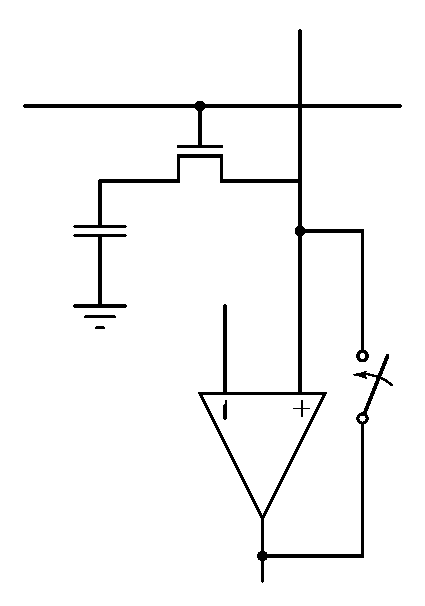
\includegraphics[scale=1]{memorie/dram_sense.eps}\\
   % translate x=640 y=576 scale 0.38
   \putbox{1.97in}{3.64in}{1.20}{$BL$}%
   \putbox{0.14in}{3.39in}{1.20}{$WL$}%
   \putbox{0.81in}{2.31in}{1.20}{$C_b$}%
   \putbox{1.39in}{1.97in}{1.20}{$\frac{V_{cc}}{2}$}%
   } % close 'parbox'
   } % close 'scalebox'
   \vspace{-\baselineskip} % this is not necessary, but looks better
\end{center}

	\caption{Cella base DRAM con circuito per refresh}
	\label{fig:dram_sense}
\end{figure}


Questo è anche utile perché, a causa delle correnti di leakage delle giunzioni polarizzate inversamente, il condensatore tende a scaricarsi nel giro di decine di \si{\milli\second}, quindi basta leggere una cella per rinfrescarla. L'operazione di lettura viene quindi effettuata anche quando non è richiesto il dato in uscita, per fare il refresh dell'informazione.

\subsection{Interfaccia esterna}
È simile a quella della SRAM: l'array si cerca di fare circa quadrato, con il decoder degli indirizzi e il multiplexer in uscita.

La differenza sta nel fatto che nella SRAM si danno tutti i bit di indirizzo insieme, mentre il bus indirizzi delle DRAM è multiplexato: gli indirizzi di riga e colonna vengono dati in due momenti successivi. Questo per ragioni storiche: quando sono nate le SRAM, non si riusciva a mettere più di qualche \si{\kilo\bit} e bastavano pochi bit per l'indirizzamento. A parità di tecnologia, però, nelle DRAM ci stavano molti più bit (centinaia di \si{\kilo\byte}). Ai quei tempi, l'unico package disponibile era il DIP e non si poteva aumentare troppo il numero di piedini per limitare i costi. Per questo motivo, dal momento che non è necessario dare contemporaneamente gli indirizzi di riga e colonna, si è scelto di multiplexare il bus. Ciò aumenta anche l'affidabilità, in quanto si riduce il numero di saldature nel chip.

\subsubsection{Segnali di controllo}
I segnali di interfaccia sono radicalmente diversi da quelli delle SRAM:
\begin{itemize}
	\item \textbf{Row Address Strobe} e \textbf{Column Address Strobe} ($\overline{RAS}$, $\overline{CAS}$): indicano alla memoria che le si sta dando l'indirizzo di riga/colonna.
	\item \textbf{Write enable} ($\overline{WE}$, $\overline{W}$, o $R/\overline{W}$): come nelle SRAM.
	\item \textbf{Output Enable} ($\overline{OE}$ o $\overline{G}$): come nelle SRAM.
\end{itemize}

\subsection{Timing diagram}
Per leggere, l'indirizzo viene dato in due parti, il segnale di scrittura sarà negato e l'output enable sarà asserito.
Mentre $\overline{RAS}$ e $\overline{CAS}$ sono inattivi, la memoria effettua la precarica per risparmiare tempo. Abbassando poi il $\overline{RAS}$, si dice alla RAM di leggere a quella riga ed essa la mette in uscita sui sense amplifier. Poi si può mettere l'indirizzo di colonna e attivare il $\overline{CAS}$ e dopo un certo tempo il dato valido sarà disponibile. Infine, questi due segnali vengono negati e il bus dati torna in alta impedenza (figura \ref{fig:dram_read_time}).
\begin{figure}[H]
	\centering
	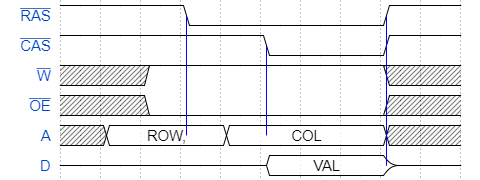
\includegraphics[width=0.7\linewidth]{memorie/dram_read_time.png}
	\caption{Timing di una DRAM in lettura}
	\label{fig:dram_read_time}
\end{figure}


Mentre nelle SRAM si può leggere di continuo, nelle DRAM non si può perché bisogna rispettare un tempo di inattività in cui la memoria effettua la precarica.

Il timing della scrittura è analogo, ma il segnale di write sarà attivo, il microprocessore metterà i dati e la scrittura avverrà sul fronte di salita del CAS.

Riguardo al refresh, tutte le righe vanno rinfrescate e quindi ogni (tempo di refresh)/(numero di righe) il processore va fermato per questa procedura. Dal punto di vista pratico, si fa una lettura, oppure una lettura senza attivare il CAS, perché tanto l'indirizzo di colonna non è necessario (\textbf{RAS-only refresh}),risparmiando così potenza evitando di attivare il multiplexer e il bus dati.

Agli albori, il controllo di queste procedure era demandato al processore. In seguito, con lo scaling tecnologico, tale controllo è stato integrato nella RAM con un contatore, permettendo di fare il refresh solo con una sequenza di comandi dall'esterno, o addirittura in modo del tutto autonomo.
\begin{datasheet}{Micron 16 Mb EDO DRAM}{}
Le DRAM si sono evolute molto di più rispetto alle SRAM, aggiungendo sempre caratteristiche aggiuntive. Ad esempio, ci sono due \textbf{clock generator}, ovvero macchine asincrone per gestire le sequenze di operazioni interne, un refresh counter ed un refresh controller.

Ci sono due segnali di CAS per selezionare su quale byte dei due della parola si vuole lavorare.

I consumi di corrente aumentano di 1000 volte tra standby e funzionamento, fino a centinaia di \si{\milli\ampere}, quindi non è vero che le DRAM consumino poco.

C'è la possibilità di lasciar fare il refresh in modo automatico alla memoria quando non utilizzata (\textbf{self refresh}), utile ad esempio durante lo stato di sospensione di un PC.

Essendo dinamica, c'è un limite anche inferiore per la frequenza: non funziona in continua.

Modalità \textbf{early write}: la scrittura avviene sull'attivazione del CAS e non sul suo fronte di salita. Il CAS deve essere comunque mantenuto attivo per un certo tempo. Tale modalità è comoda lavorando con macchine a stati perché si può dare nello stesso stato l'indirizzo di colonna e il dato da scrivere.

Modalità \textbf{read-modify-write}: si fa una lettura normale, si toglie output enable, si mette il dato da scrivere sul bus e si dà il segnale di write. Il tutto senza muovere RAS e CAS. È utile per generare dei \textbf{semafori} software, ovvero per eseguire operazioni indivisibili.

Modalità \textbf{page mode} o \textbf{EDO} (Extended Data Output): l'operazione più lenta è l'estrazione della riga, quindi tale modalità permette di leggere più colonne consecutive all'interno della stessa riga, muovendo solamente il CAS e mantenendo il RAS sempre attivo. Ciò permette di leggere parole consecutive fino a 4 volte più velocemente rispetto ad una lettura normale. È utile ad esempio nelle cache.

Modalità \textbf{CBR refresh} (CAS Before RAS): attivando prima il CAS e poi il RAS (al contrario del normale), la memoria fa un ciclo di refresh in modo autonomo, facendo risparmiare hardware.

Modalità \textbf{hidden refresh}: dopo una lettura normale, togliendo il RAS mantenendo il CAS attivo, la memoria fa un ciclo di refresh, mantenendo però i dati in uscita.

Ci sono più piedini di alimentazione e massa, in modo che la corrente impulsiva venga dispersa in modo migliore.
\end{datasheet}

\subsection{DRAM sincrone (SDRAM)}
Migliorando la tecnologia e potendo avere accessi più veloci, si è deciso di introdurre un clock e dei latch di pipeline tra i vari blocchi. La cella base è identica, cambia solo l'interfacciamento esterno.

In seguito sono state introdotte le SDRAM DDR (Double Data Rate) e quindi quelle precedenti sono state rinominate SDR (Single Data Rate).

Così come per le SSRAM, non solo è stato introdotto un clock, ma si è anche aumentata la complessità dell'interfaccia del circuito per ottenere un miglioramento delle prestazioni.

\begin{datasheet}{Micron 256 Mb SDR SDRAM}{}
In questo esempio il chip ha 32 Mword da 8 bit ciascuna. I segnali di controllo sono gli stessi della DRAM asincrona, con l'aggiunta di un clock, un clock enable e un chip select.

Gli indirizzi vengono messi in un registro, così come i dati in ingresso o uscita: sono stadi di pipe.

Ci sono quattro decoder di riga e colonna, così come quattro array di memoria, ovvero si è usata la tecnica del \textbf{banking}: così si può evitare il tempo di precharge, leggendo da un banco, mentre si sta facendo la precarica in una altro e il refresh di un altro ancora. La memoria è disponibile in modo continuo se si accede a banchi diversi, il che è possibile salvando parole contigue su banchi diversi.

C'è anche un refresh counter, perché il refresh è effettuato dalla memoria stessa.

Il tempo di refresh è simile a quello delle DRAM asincrone perché, scalando la tecnologia, si riducono le dimensioni dei MOS e quindi il leakage, ma d'altro canto si riduce anche la capacità di canale, quindi il tempo di scarica rimane simile.

Similmente, anche i tempi di accesso non migliorano molto perché scalando la cella base la quantità di elettroni immagazzinati nella capacità diminuisce e quindi tutte le capacità scalano e la velocità con cui il dato viene trasferito sulla bitline non cambia molto.

Le frequenze sono in linea con quelle dei processori Intel 386 e 486 dell'epoca. Tuttavia, può capitare che il processore vada ad una frequenza minore, quindi si rischia di sottoutilizzare il chip di memoria: se la RAM, ad esempio, può dare un dato in 4 colpi di clock a \SI{100}{\mega\hertz}, significa che ogni \SI{40}{\nano\second} potenzialmente c'è un dato disponibile, ma usando un clock a \SI{50}{\mega\hertz}, questo tempo assoluto è doppio a parità di colpi di clock e quindi la memoria non è ben sfruttata. Per ovviare a questo problema, si è introdotta la possibilità di cambiare la profondità della pipeline: al clock nominale, si passa da tutti i registri, a frequenze minori alcuni invece vengono bypassati. 

Questa funzione, come altre, va configurata tramite il \textbf{mode register}, gestito dalla logica di interna al chip. In effetti, i segnali di controllo hanno lo stesso nome delle DRAM asincrone, ma il significato è diverso: sono in realtà 4 bit di un comando, come se fosse un processore con un ISA di 16 istruzioni. La RAM ad ogni colpo di clock legge tale comando che scatenerà una sequenza di eventi nella pipeline.

Ad esempio, esiste un comando di precharge, per effettuare la precarica di un determinato banco, oppure un comando analogo per il refresh.

Le SDRAM sono oggetti complessi e in quanto tali hanno bisogno di una sequenza di inizializzazione all'avvio, altrimenti la RAM funziona a caso. Non è un problema dal momento che le RAM dinamiche vengono utilizzate spesso e volentieri in sistemi in cui la potenza di calcolo abbonda, anzi, alcuni microcontrollori hanno un'interfaccia DRAM che si occupa automaticamente di tale inizializzazione. I passi fondamentali sono:
\begin{itemize}
	\item Dare la tensione di alimentazione.
	\item Dare il clock enable e mantenerlo finché le uscite non sono stabili. Tale segnale serve soprattutto per risparmiare energia quando la memoria non è utilizzata.
	\item Fornire un clock stabile. Finché non si arriva a regime, il segnale è una sinusoide analogica ed il tempo per arrivare a regime dipende dalla potenza disponibile, ma può essere dell'ordine di decine di \si{\micro\second} per oscillatori al quarzo standard, mentre sale per quelli a bassissima potenza.
	\item Aspettare altri \SI{100}{\micro\second} affinché al RAM generi delle tensioni ausiliarie con circuiti a capacità commutate che utilizzano il clock come segnale di sincronizzazione.
	\item In questo periodo dare clock enable e almeno un comando NOP per resettare tutto.
	\item Dare il comando di precharge a tutti i banchi.
	\item Aspettare che tutto sia precaricato.
	\item Dare per due volte il comando di refresh e aspettare.
	\item Configurare il mode register che all'avvio è in una configurazione ignota. Di solito questa programmazione si fa una volta per tutte.
\end{itemize}

Il mode register ha 13 bit e viene programmato dando il comando opportuno e il suo contenuto sul bus indirizzi (non sul bus dati). Per garantire la compatibilità sia indietro che avanti, alcuni bit o combinazioni di bit non sono utilizzate e quindi vanno programmate a 0. Bisogna evitare di lasciare eventuali ``tombini aperti'' per non avere problemi futuri, se proprio è necessario bisogna segnalarlo con delle note nel progetto.

La CAS latency permette di impostare, come accennato prima, il numero di registri di pipe. Solo due combinazioni dei tre bit sono disponibili, le altre sono riservate.

La RAM in \textbf{burst mode} permette di leggere parole successive sulla stessa riga e la lunghezza di tale burst può essere impostata. Se tale numero di parole desiderato non è presente tra le impostazioni, si può decidere di leggere una pagina intera ed interrompere al momento voluto con il comando \textsc{burst terminate}.

I bit di operating mode permettono di impostare solo la modalità di funzionamento normale, le altre configurazioni sono probabilmente utilizzate dal costruttore in fase di testing.

Dal momento che statisticamente le letture sono più delle scritture, magari non è necessario scrivere in burst e quindi si può impostare solo la lettura a burst.

Interessante è notare che il comando \textsc{active} dal timing diagram porti in uscita il dato in 3 colpi di clock, ma in realtà è da soddisfare un tempo di propagazione assoluto, non in termini di colpi di clock. Quindi magari usando un clock più lento, per coprire lo stesso tempo, bastano meno colpi di clock.

I piedini di alimentazione positivo e negativo sono disposti vicini per i grossi buffer di uscita. I circuiti CMOS quando commutando assorbono una corrente impulsiva passando nella zona lineare, dato che le piste sono delle induttanze e quindi dei circuiti aperti in transitorio, la tensione scende. Per risolvere si mette un \textbf{condensatore di disaccoppiamento}. Avendo la piedinatura fatta in quel modo, tale condensatore si può mettere direttamente vicino ai piedini.

Bisogna sottolineare che, nonostante i livelli di pipe, la latenza assoluta rimane simile a quella delle altre RAM, perché l'array di memoria non scala molto come velocità.
\end{datasheet}

\begin{datasheet}{Micron 2 Gb DDR3 SDRAM}{}\label{ds:ddr3}
La frequenza di lavoro arriva fino a \SI{1866}{\mega\hertz}, con una CAS latency pari a 13. Ultimamente più che sulla frequenza massima si cerca di spingere sulla densità della memoria. In realtà tale frequenza non è quella del clock, che infatti ha un periodo di \SI{1.07}{\nano\second}, ma è il numero di parole al secondo, cioè, essendo Double Data Rate, il doppio della frequenza di clock.

La latenza totale in realtà non è migliorata molto rispetto alle RAM più vecchie (circa \SI{40}{\nano\second} piuttosto che circa \SI{70}{\nano\second}), perché l'array di memoria rimane sempre il collo di bottiglia. Anzi, la memoria più veloce, avendo più stadi di pipe, ha una latenza più grande di quella più lenta. Non sempre comprare il componente più veloce è un vantaggio. 

Anche i consumi di corrente sono sempre simili, nell'ordine di \SI{100}{\milli\ampere}.

Il fatto di andare ad alta velocità significa innanzitutto che i driver di uscita devono essere adattati: la loro impedenza si può impostare nel mode register. In secondo luogo, tutte le piste del data bus che vanno dalla memoria al processore devono essere lunghe uguale: i fili fanno percorsi diversi per adattare la loro lunghezza.

DDR significa che per ogni colpo di clock si trasferiscono due word, aumentando la banda. In un circuito SDR, un dato può commutare al massimo con frequenza pari a metà di quella del clock, perché può avere una transizione solo ad ogni fronte di salita. Ma quindi il mezzo fisico è sottoutilizzato perché può tollerare un clock ad una certa frequenza, ma tutti gli altri segnali vanno alla metà. Per un circuito DDR, invece, i dati vanno alla stessa frequenza del clock. 

Ma come si fanno a campionare? Internamente bisogna generare un clock a frequenza doppia. Ma a frequenze tali, anche un piccolo ritardo sui fili, rischia di rendere il sistema asincrono. Allora si è deciso che la RAM, oltre al dato, mandi anche un segnale DQS, ovvero uno strobe (differenziale) che dica al processore quando campionare il dato.
\begin{figure}[hbtp]
	\centering
	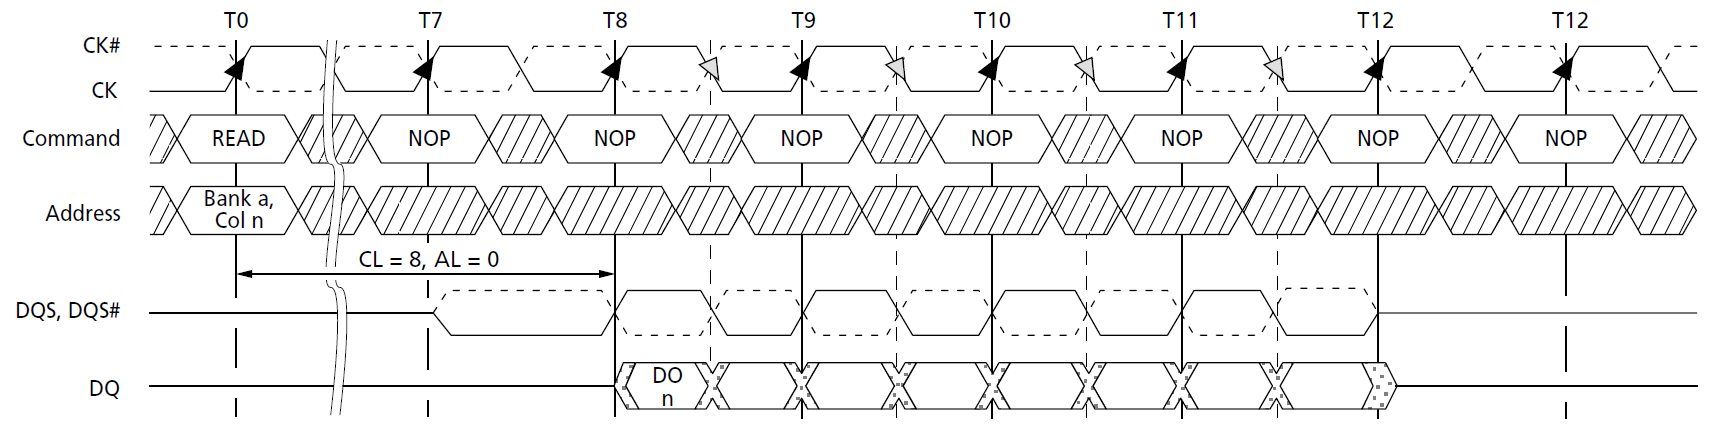
\includegraphics[width=\linewidth]{memorie/ddr_timing}
	\caption{Timing della memoria in lettura}
\end{figure}
\end{datasheet}

\section{ROM}
In origine le ROM erano effettivamente memorie che potevano essere esclusivamente lette, il cui contenuto veniva deciso in fase di produzione (\textbf{masked ROM}), mettendo o no un contatto ad ogni incrocio tra wordline e bitline. 

Ad esempio, si poteva mettere un diodo (e non un MOS perché la tecnologia era bipolare) per avere un 1 logico ed i buffer di uscita in fondo alla colonna con una resistenza di pull-down verso massa, per mantenere uno 0 in assenza di contatto (\ref{fig:masked_rom}). Attivando una riga si attivano tutte le colonne. In realtà si mettevano tutti i diodi e si connettevano oppure no in base al contenuto, ovvero, solo la maschera dei contatti cambiava da una ROM ad un'altra. 

Il costo della maschera aveva però un impatto enorme sul costo del singolo chip, allora si è cercato di fare i chip tutti uguali con la possibilità per l'utente di programmarli.

\begin{figure}[hbtp]
	\centering
	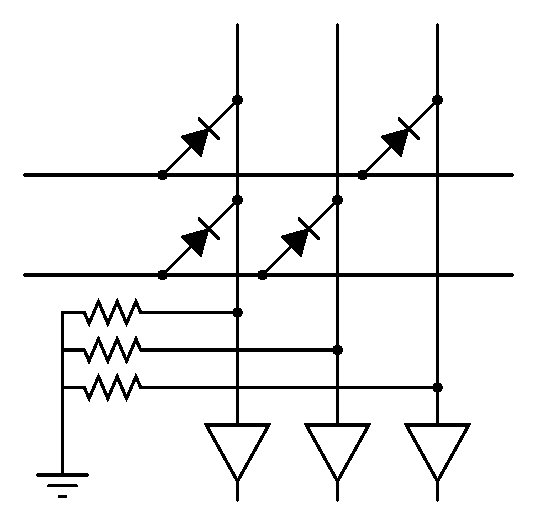
\includegraphics[scale=0.6]{memorie/masked_rom}
	\caption{Masked ROM con diodi}
	\label{fig:masked_rom}
\end{figure}

\subsection{PROM (Programmable ROM)}
In serie al diodo si mette un fusibile ed il cliente li va a bruciare oppure no con un programmatore di PROM. Lo svantaggio sta nel fatto che i fusibili non possono essere testati e quindi, data la resa non unitaria, c'è una probabilità non nulla che il chip sia difettoso.

L'unica soluzione è essere conservativi con il processo tecnologico, il che porta però ad area e quindi costi maggiori.

Inoltre, all'evaporazione del fusibile il metallo si va a depositare in altri luoghi del chip, rischiando di creare cortocircuiti.

Infine, il chip è \textbf{OTP} (One Time Programmable), perché non è cancellabile.

\subsection{EPROM (Erasable Programmable ROM)}
Alcuni di questi problemi sono stati risolti con l'avvento dei MOS a gate flottante (\textbf{FAMOS}, figura \ref{fig:famos}). La differenza rispetto ad un MOS tradizionale sta nel fatto che sotto al gate ordinario c'è un secondo gate completamente isolato. Nel calcolo della tensione di soglia, ora, rientra la quantità di carica accumulata in totale in entrambi i gate. Quindi, cambiando la carica nel gate flottante, si può variare la tensione di soglia. Essendo, inoltre, che l'ossido di gate è un ottimo isolante, le cariche intrappolate nel floating gate non scappano facilmente, anzi possono restare intrappolate per anni.

\begin{figure}[hbtp]
	\centering
	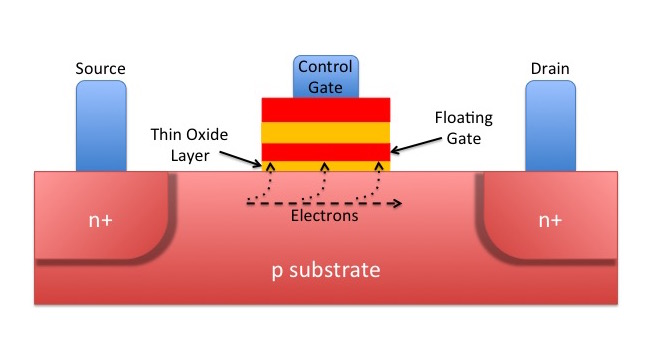
\includegraphics[width=0.4\linewidth]{memorie/famos.jpg}
	\caption{Floating gate MOS}
	\label{fig:famos}
\end{figure}

In definitiva, si può fare in modo che la tensione di alimentazione stia tra la tensione di soglia del MOS non programmato (senza elettroni nel floating gate) e quella del MOS programmato. Così, a seconda dello stato del MOS, esso conduce oppure no quando viene applicata \vcc (figura \ref{fig:vth_famos})

\begin{figure}[hbtp]
	\centering
	% This file was created by matlab2tikz.
%
%The latest updates can be retrieved from
%  http://www.mathworks.com/matlabcentral/fileexchange/22022-matlab2tikz-matlab2tikz
%where you can also make suggestions and rate matlab2tikz.
%
\begin{tikzpicture}[scale=0.7]

\begin{axis}[%
axis lines = left,
width=4.521in,
height=3.423in,
at={(0.758in,0.624in)},
scale only axis,
xmin=0,
xmax=6,
xtick={1,2,3},
xticklabels={{$\text{V}_{\text{th}_\text{A}}$},{$\text{V}_{\text{cc}}$},{$\text{V}_{\text{th}_\text{B}}$}},
xlabel style={font=\color{white!15!black}},
xlabel={$\text{V}_{\text{GS}}$},
ymin=0,
ymax=9,
ytick={\empty},
ylabel style={font=\color{white!15!black}},
ylabel={$\text{I}_\text{D}$},
axis background/.style={fill=white},
%legend style={legend cell align=left, align=left, draw=white!15!black}
]
\addplot [color=black]
  table[row sep=crcr]{%
1	0\\
1.03030303030303	0.000918273645546371\\
1.06060606060606	0.00367309458218548\\
1.09090909090909	0.00826446280991734\\
1.12121212121212	0.0146923783287419\\
1.15151515151515	0.0229568411386593\\
1.18181818181818	0.0330578512396694\\
1.21212121212121	0.0449954086317723\\
1.24242424242424	0.0587695133149679\\
1.27272727272727	0.0743801652892562\\
1.3030303030303	0.0918273645546372\\
1.33333333333333	0.111111111111111\\
1.36363636363636	0.132231404958678\\
1.39393939393939	0.155188246097337\\
1.42424242424242	0.179981634527089\\
1.45454545454545	0.206611570247934\\
1.48484848484848	0.235078053259871\\
1.51515151515152	0.265381083562902\\
1.54545454545455	0.297520661157025\\
1.57575757575758	0.331496786042241\\
1.60606060606061	0.367309458218549\\
1.63636363636364	0.40495867768595\\
1.66666666666667	0.444444444444444\\
1.6969696969697	0.485766758494031\\
1.72727272727273	0.528925619834711\\
1.75757575757576	0.573921028466483\\
1.78787878787879	0.620752984389348\\
1.81818181818182	0.669421487603306\\
1.84848484848485	0.719926538108356\\
1.87878787878788	0.7722681359045\\
1.90909090909091	0.826446280991736\\
1.93939393939394	0.882460973370064\\
1.96969696969697	0.940312213039486\\
2	1\\
2.03030303030303	1.06152433425161\\
2.06060606060606	1.12488521579431\\
2.09090909090909	1.1900826446281\\
2.12121212121212	1.25711662075298\\
2.15151515151515	1.32598714416896\\
2.18181818181818	1.39669421487603\\
2.21212121212121	1.4692378328742\\
2.24242424242424	1.54361799816345\\
2.27272727272727	1.6198347107438\\
2.3030303030303	1.69788797061524\\
2.33333333333333	1.77777777777778\\
2.36363636363636	1.8595041322314\\
2.39393939393939	1.94306703397613\\
2.42424242424242	2.02846648301194\\
2.45454545454545	2.11570247933884\\
2.48484848484848	2.20477502295684\\
2.51515151515152	2.29568411386593\\
2.54545454545455	2.38842975206612\\
2.57575757575758	2.48301193755739\\
2.60606060606061	2.57943067033976\\
2.63636363636364	2.67768595041322\\
2.66666666666667	2.77777777777778\\
2.6969696969697	2.87970615243343\\
2.72727272727273	2.98347107438017\\
2.75757575757576	3.089072543618\\
2.78787878787879	3.19651056014692\\
2.81818181818182	3.30578512396694\\
2.84848484848485	3.41689623507805\\
2.87878787878788	3.52984389348026\\
2.90909090909091	3.64462809917355\\
2.93939393939394	3.76124885215794\\
2.96969696969697	3.87970615243343\\
3	4\\
3.03030303030303	4.12213039485767\\
3.06060606060606	4.24609733700643\\
3.09090909090909	4.37190082644628\\
3.12121212121212	4.49954086317723\\
3.15151515151515	4.62901744719926\\
3.18181818181818	4.7603305785124\\
3.21212121212121	4.89348025711662\\
3.24242424242424	5.02846648301194\\
3.27272727272727	5.16528925619835\\
3.3030303030303	5.30394857667585\\
3.33333333333333	5.44444444444445\\
3.36363636363636	5.58677685950413\\
3.39393939393939	5.73094582185491\\
3.42424242424242	5.87695133149679\\
3.45454545454545	6.02479338842975\\
3.48484848484848	6.17447199265381\\
3.51515151515152	6.32598714416896\\
3.54545454545455	6.47933884297521\\
3.57575757575758	6.63452708907254\\
3.60606060606061	6.79155188246097\\
3.63636363636364	6.9504132231405\\
3.66666666666667	7.11111111111111\\
3.6969696969697	7.27364554637282\\
3.72727272727273	7.43801652892562\\
3.75757575757576	7.60422405876951\\
3.78787878787879	7.7722681359045\\
3.81818181818182	7.94214876033058\\
3.84848484848485	8.11386593204775\\
3.87878787878788	8.28741965105602\\
3.90909090909091	8.46280991735537\\
3.93939393939394	8.64003673094582\\
3.96969696969697	8.81910009182736\\
4	9\\
};
%\addlegendentry{data1}

\addplot [color=black]
  table[row sep=crcr]{%
3	0\\
3.03030303030303	0.000918273645546371\\
3.06060606060606	0.00367309458218548\\
3.09090909090909	0.00826446280991734\\
3.12121212121212	0.0146923783287419\\
3.15151515151515	0.0229568411386593\\
3.18181818181818	0.0330578512396694\\
3.21212121212121	0.0449954086317722\\
3.24242424242424	0.0587695133149678\\
3.27272727272727	0.0743801652892561\\
3.3030303030303	0.0918273645546374\\
3.33333333333333	0.111111111111111\\
3.36363636363636	0.132231404958678\\
3.39393939393939	0.155188246097337\\
3.42424242424242	0.179981634527089\\
3.45454545454545	0.206611570247934\\
3.48484848484848	0.235078053259871\\
3.51515151515152	0.265381083562902\\
3.54545454545455	0.297520661157025\\
3.57575757575758	0.331496786042241\\
3.60606060606061	0.367309458218549\\
3.63636363636364	0.40495867768595\\
3.66666666666667	0.444444444444444\\
3.6969696969697	0.485766758494032\\
3.72727272727273	0.528925619834711\\
3.75757575757576	0.573921028466483\\
3.78787878787879	0.620752984389348\\
3.81818181818182	0.669421487603306\\
3.84848484848485	0.719926538108356\\
3.87878787878788	0.7722681359045\\
3.90909090909091	0.826446280991736\\
3.93939393939394	0.882460973370064\\
3.96969696969697	0.940312213039486\\
4	1\\
4.03030303030303	1.06152433425161\\
4.06060606060606	1.12488521579431\\
4.09090909090909	1.1900826446281\\
4.12121212121212	1.25711662075298\\
4.15151515151515	1.32598714416896\\
4.18181818181818	1.39669421487603\\
4.21212121212121	1.4692378328742\\
4.24242424242424	1.54361799816345\\
4.27272727272727	1.6198347107438\\
4.3030303030303	1.69788797061524\\
4.33333333333333	1.77777777777778\\
4.36363636363636	1.8595041322314\\
4.39393939393939	1.94306703397613\\
4.42424242424242	2.02846648301194\\
4.45454545454546	2.11570247933884\\
4.48484848484848	2.20477502295684\\
4.51515151515152	2.29568411386593\\
4.54545454545454	2.38842975206611\\
4.57575757575758	2.48301193755739\\
4.60606060606061	2.57943067033976\\
4.63636363636364	2.67768595041322\\
4.66666666666667	2.77777777777778\\
4.6969696969697	2.87970615243343\\
4.72727272727273	2.98347107438017\\
4.75757575757576	3.089072543618\\
4.78787878787879	3.19651056014692\\
4.81818181818182	3.30578512396694\\
4.84848484848485	3.41689623507805\\
4.87878787878788	3.52984389348026\\
4.90909090909091	3.64462809917355\\
4.93939393939394	3.76124885215794\\
4.96969696969697	3.87970615243343\\
5	4\\
5.03030303030303	4.12213039485767\\
5.06060606060606	4.24609733700643\\
5.09090909090909	4.37190082644628\\
5.12121212121212	4.49954086317723\\
5.15151515151515	4.62901744719926\\
5.18181818181818	4.7603305785124\\
5.21212121212121	4.89348025711662\\
5.24242424242424	5.02846648301194\\
5.27272727272727	5.16528925619835\\
5.3030303030303	5.30394857667585\\
5.33333333333333	5.44444444444445\\
5.36363636363636	5.58677685950413\\
5.39393939393939	5.73094582185491\\
5.42424242424242	5.87695133149678\\
5.45454545454546	6.02479338842975\\
5.48484848484848	6.17447199265381\\
5.51515151515152	6.32598714416896\\
5.54545454545454	6.4793388429752\\
5.57575757575758	6.63452708907255\\
5.60606060606061	6.79155188246097\\
5.63636363636364	6.9504132231405\\
5.66666666666667	7.11111111111111\\
5.6969696969697	7.27364554637282\\
5.72727272727273	7.43801652892562\\
5.75757575757576	7.60422405876951\\
5.78787878787879	7.7722681359045\\
5.81818181818182	7.94214876033058\\
5.84848484848485	8.11386593204775\\
5.87878787878788	8.28741965105602\\
5.90909090909091	8.46280991735537\\
5.93939393939394	8.64003673094582\\
5.96969696969697	8.81910009182736\\
6	9\\
};
%\addlegendentry{data2}

\legend={\empty};

\end{axis}
\end{tikzpicture}%
	\caption{Diverse tensioni di soglia in un FAMOS}
	\label{fig:vth_famos}
\end{figure}

Si possono iniettare cariche nel floating gate con tensioni elevate (10-25 V) che superino la barriera di potenziale del diagramma a bande: il campo elettrico elevato accelera gli elettroni e li devia e, se la loro energia cinetica è sufficiente, rimangono intrappolati nel gate.

Nella cella base (figura \ref{fig:eprom}), attivando la wordline, se il MOS conduce la bitline viene portata a 0, altrimenti rimane a 1.

\begin{figure}[hbtp]
	\centering
	% XCircuit output "eprom.tex" for LaTeX input from eprom.eps
\def\putbox#1#2#3#4{\makebox[0in][l]{\makebox[#1][l]{}\raisebox{\baselineskip}[0in][0in]{\raisebox{#2}[0in][0in]{\scalebox{#3}{#4}}}}}
\def\rightbox#1{\makebox[0in][r]{#1}}
\def\centbox#1{\makebox[0in]{#1}}
\def\topbox#1{\raisebox{-0.60\baselineskip}[0in][0in]{#1}}
\def\midbox#1{\raisebox{-0.20\baselineskip}[0in][0in]{#1}}
\begin{center}
   \scalebox{0.6}{
   \normalsize
   \parbox{2.04688in}{
   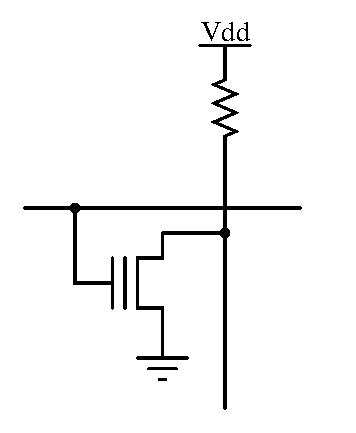
\includegraphics[scale=1]{memorie/eprom.eps}\\
   % translate x=608 y=256 scale 0.38
   \putbox{1.56in}{2.06in}{1.20}{$R_{PU}$}%
   } % close 'parbox'
   } % close 'scalebox'
   \vspace{-\baselineskip} % this is not necessary, but looks better
\end{center}

	\caption{Cella base EPROM}
	\label{fig:eprom}
\end{figure}

Per riportare i MOS nello stato iniziale, si illumina il chip con una luce ultravioletta (cioè fotoni energetici) che eccita gli elettroni che possono uscire fuori dal floating gate, con probabilità non nulla. Dal momento che questo è un processo statistico, il tempo di cancellazione può arrivare fino ad un'ora.

Inoltre, il package deve avere una finestra di quarzo, in quanto trasparente agli UV, che però non si salda con la plastica e quindi necessita di ceramica, il che fa aumentare notevolmente il costo. Spesso, per ridurre i costi totali, si sviluppa su una EPROM con il package in ceramica in modo da poter cancellare, mentre poi il prodotto finito si può mettere in un chip con il package plastico (\textbf{OTP EPROM}).

\subsection{EEPROM (Electrically Erasable Programmable ROM)}
La limitazione della EPROM sta ovviamente nel lunghissimo tempo di cancellazione, che viene risolto con lo scaling tecnologico che permette di produrre transistor con gate molto sottili, da cui gli elettroni si possono togliere per effetto tunnel.

Quindi le memorie non volatili con le EEPROM sono diventate utili per modificarne il contenuto anche \emph{on-field}. Tali memorie possono quindi essere definite \emph{mostly read}, in quanto permettono all'occorrenza anche di essere scritte.

Le prime EEPROM potevano essere scritte solo un centinaio di volte, perché gli elettroni che escono dal gate sbattono contro il reticolo e creano dei livelli trappola nel diagramma a bande, spostando così le tensioni di gate e ad un certo punto danneggiando permanentemente il transistor, che smette di accendersi o non si spegne più. 

\chapter{Memorie: Flash}
Negli anni 2000, Intel realizza delle EEPROM particolari, apportando delle modifiche architetturali ed inventa così le memorie flash. Tali memorie sono delle EEPROM a tutti gli effetti, ma presentano numerosi vantaggi come la maggiore densità di bit e le migliori prestazioni. Il numero di cicli di scrittura e cancellazione, inoltre, può arrivare fino ad 1 milione.

Lo svantaggio è che, mentre nelle EEPROM si può cancellare una singola word, nelle flash la scrittura può essere a word, ma la cancellazione deve per forza essere fatta a blocchi, magari di qualche \si{\kilo\byte}. 

Le EEPROM si usano ancora al giorno d'oggi solo più in piccoli tagli, per memorizzare informazioni quali parametri di configurazione o numeri di identificazione.

Esistono due tipi fondamentali di flash: le NOR flash (quelle primigenie) e le NAND flash (quelle più moderne). La flash originale si chiama NOR in quanto la sua struttura ricorda una porta NOR a due ingressi in tecnologia CMOS, al contrario le flash più recenti hanno una disposizione dei transistor simile a quella di una porta NAND. Solitamente in ogni sistema c'è almeno un po' di NOR flash (figure \ref{fig:nand_nor}).
\begin{figure}[hbtp]
	\centering
	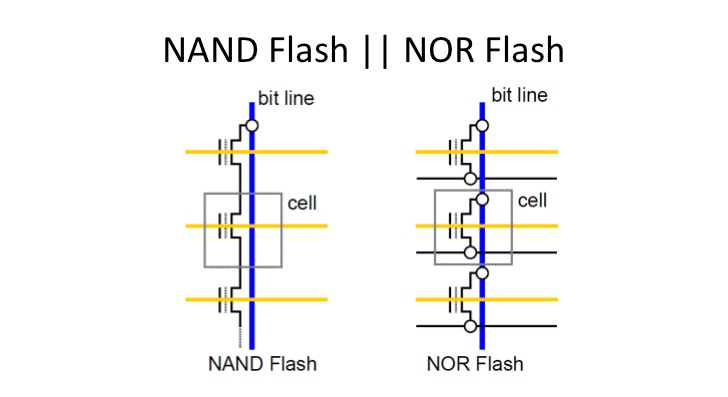
\includegraphics[width=0.6\linewidth]{memorie/nand_nor_flash.jpg}
	\caption{Struttura di NAND e NOR flash}
	\label{fig:nand_nor}
\end{figure}


\section{NOR flash}
Per ragioni storiche, l'interfaccia esterna della NOR flash è del tutto simile a quella di una RAM, ovvero presenta gli stessi segnali di controllo. Inoltre, anche il ciclo di lettura è identico a quello di una RAM, anche in termini di tempistiche.

Il ciclo di scrittura, invece, richiede del tempo che può essere non costante e per questo motivo i segnali di controllo, in scrittura, non servono a scrivere direttamente dentro l'array di memoria, ma impartiscono dei comandi ad un'unità di controllo interna alla flash, che si occupa di completare il processo di scrittura in seguito internamente.

In qualsiasi sistema embedded ci deve essere una memoria non volatile in cui salvare il codice che il microprocessore deve eseguire al momento del boot. Dal momento che la NOR flash supporta letture casuali, questa è proprio la sua applicazione tipica. Essa quindi, in generale, viene usata per salvare il codice eseguibile, al contrario della RAM che viene impiegata soprattutto per memorizzare i dati.

\begin{datasheet}{Numonyx Embedded NOR flash Memory}{}
NOR flash da 32 a 256 Mbit, sufficienti per un distribuzione Linux embedded. L'array è diviso in blocchi tutti uguali, ma potrebbero anche essere diversi. 

Il tempo di accesso è nell'ordine di \SI{80}{\nano\second}, mentre la scrittura è molto più lenta (\SI{4}{\micro\second}).

Può essere utile impedire ai malintenzionati di modificare il contenuto della flash e per questo esiste un registro in cui si può scrivere un CRC che viene controllato prima di modificare i dati.

Le scritture e cancellazioni sono bloccate per sicurezza quando l'alimentazione non è stabile.

\textbf{Program and erase suspend}: per cancellare o scrivere un blocco, si dà un comando all'unità di controllo della flash, ma essa deve scollegare l'array per poter applicare le tensioni necessarie e quindi la memoria non può più essere letta e la flash scompare dal bus. O si blocca il processore per un tempo lungo, oppure si scrive in RAM (o in una seconda flash) la subroutine di cancellazione o scrittura. Questa funzione permette di interrompere la programmazione della flash per un breve periodo di tempo per leggere dei dati, utile ad esempio per servire degli interrupt mentre si sta scrivendo o cancellando.

\textbf{FDI} (Flash Data Integrator) e \textbf{CFI} (Common Flash Interface): nella memoria c'è una tabella che contiene tutte le informazioni relative alla flash, in modo che il software la possa leggere e capire come interfacciarsi con essa. Tale tabella e la sua interfaccia sono standard.

Nello schema a blocchi, il multiplexer di uscita può far passare i dati oppure la query (CFI) oppure lo \textbf{status register} (che contiene informazioni di stato o errore, figura \ref{fig:status_register}) oppure l'identifier register. Quindi la flash è sempre in grado di soddisfare una richiesta di lettura.

Per la scrittura, bisogna negare il segnale di output enable, al contrario della RAM in cui era un don't care. Questo per sicurezza, in modo da evitare che un disturbo attivi output enable.

All'accensione ogni lettura è una lettura dall'array e ogni scrittura è un invio di un comando alla control unit. Questo perché così un microprocessore all'accensione può solo andare a leggere il codice da eseguire, quindi la flash deve essere pronta.

Per inviare alcuni comandi non basta un ciclo di scrittura sul bus, ma ne serve un secondo consecutivo di conferma. Solitamente questi sono comandi pericolosi che portano ad una modifica permanente del dispositivo.

\begin{figure}[hbtp]
	\centering
	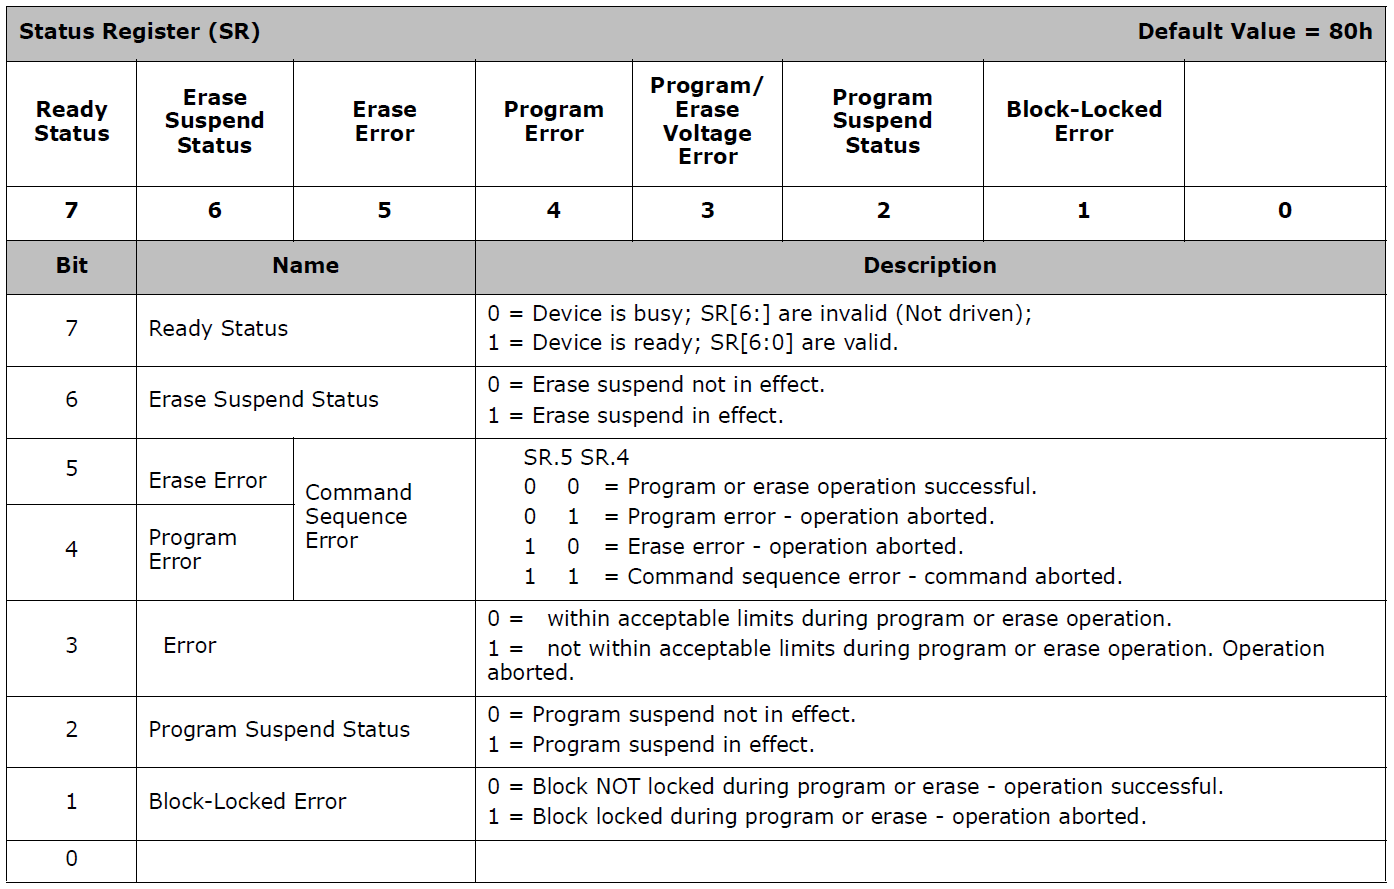
\includegraphics[width=\linewidth]{memorie/flash_status_register.png}
	\caption{Status register}
	\label{fig:status_register}
\end{figure}

Dando il comando di query alla CFI, le successive letture leggono il contenuto della tabella. I primi caratteri sono Q, R ed Y e servono per capire se si sta effettivamente leggendo la tabella.
\end{datasheet}

\section{NAND flash}
Le NAND flash sono invece più simili ad un Hark Disk, in quanto l'accesso in lettura è sequenziale. Per simulare la modalità ad accesso casuale, bisogna prima copiare il contenuto della memoria in RAM (tecnica chiamata \textbf{shadowing}). Queste memorie non sono quindi particolarmente adatte a memorizzare del codice eseguibile, dal momento che le architetture Von Neumann richiedono che esso sia salvato su una memoria indirizzabile.

A maggior ragione quindi, le NAND flash non vengono utilizzate per fare il boot in un sistema basato su microcontrollore.

\subsection{Struttura interna}
\begin{figure}[hbtp]
	\centering
	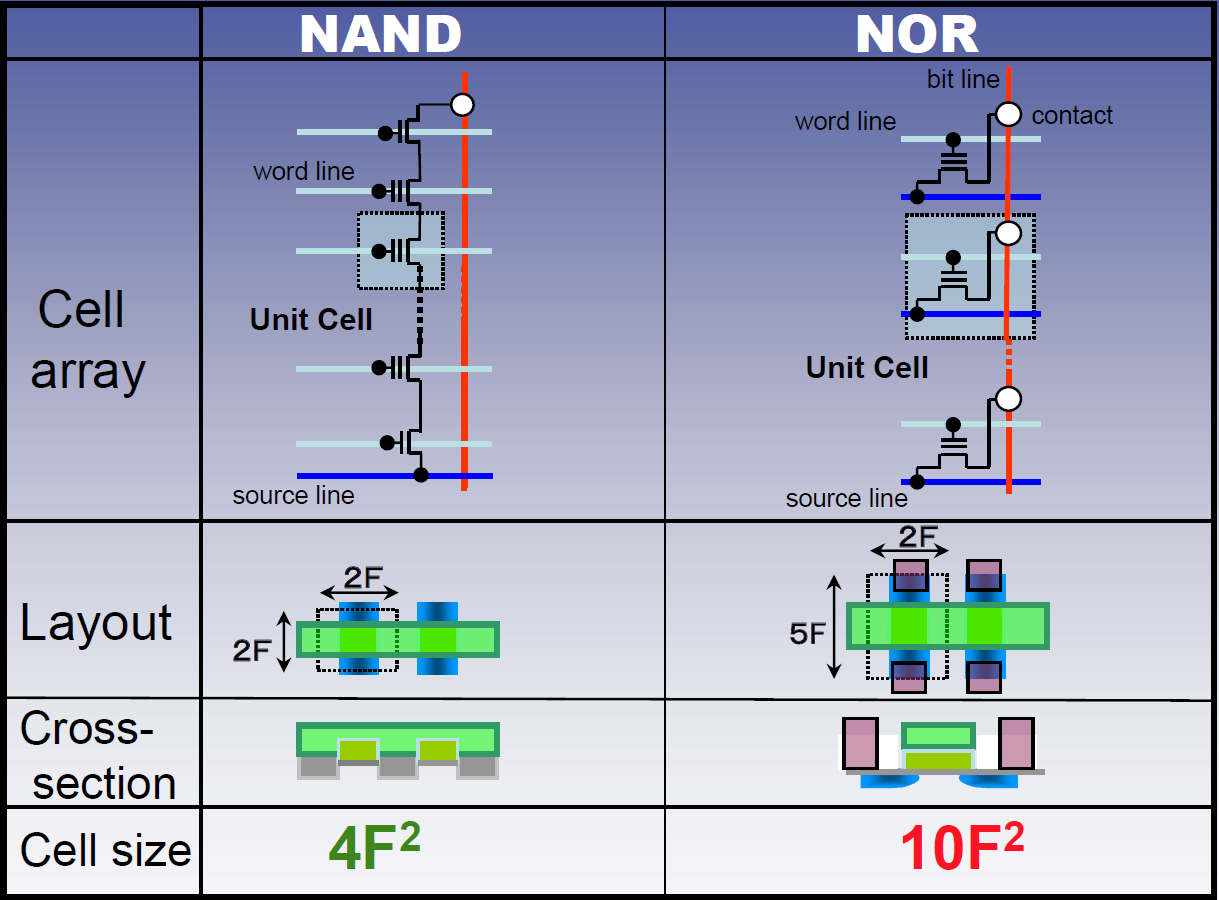
\includegraphics[width=0.6\textwidth]{memorie/jc_struttura_interna}
	\caption{Struttura interna di NAND e NOR flash}
	\label{fig:jc_struttura_interna}
\end{figure}
Come si può vedere dalla figura \ref{fig:jc_struttura_interna}, nella NOR flash, il source dei MOS è collegato ad una linea conduttrice che in lettura è a massa per ogni transistor, mentre in scrittura si porta a 1 logico per i transistor che non devono essere programmati. I MOS sono disposti secondo uno schema wired-OR: per leggere una cella si attiva una wordline e di conseguenza la bitline viene portata a 0 o lasciata invariata a seconda che il MOS sia programmato o no.

Nella NAND flash, invece, i transistori sono in serie e quindi per effettuare una lettura su una cella si accendono tutti tranne quello della cella di interesse: se quel MOS conduce, la bitline va a 0, altrimenti rimane al suo valore di precarica. Il primo e l'ultimo MOS della catena non sono floating gate, ma normali perché servono solamente a collegare la serie di MOS alla bitline o alla linea conduttiva dei source.

Le NAND flash hanno successo proprio perché limitano il numero di connessioni tra bitline e diffusioni, che sono particolarmente ingombranti, e quindi permettono di avere un'alta densità, grazie ad una riduzione del 60\% dell'area rispetto ad una NOR flash. Per questo motivo, le NAND flash riescono ad avvicinarsi alle capacità tipiche degli HDD.

Lo svantaggio di avere dispositivi così densi, è l'alta probabilità di avere dei bit che non funzionano a causa di difetti in fase di produzione. Per questo motivo, per non dover scartare un numero troppo elevato di chip, si aggiungono bit in più rispetto a quelli necessari in modo da avere ridondanza.

\begin{tcolorbox}[breakable]
\textbf{HDD magnetici}\\
Sono formati da un disco rotante una tempo composto di alluminio, ma oggi di vetro data la sua maggiore rigidità strutturale, necessaria in quanto le velocità superficiali di rotazione possono arrivare fino a \SI{150}{\kilo\meter\per\hour}. Su questo disco viene depositato un materiale ferrimagnetico in modo da poter memorizzare un bit di informazione in base al verso della magnetizzazione di un certo numero di domini di Weiss.

Per leggere tale informazione, scritta in tracce concentriche, un braccio meccanico fornito di una testina scorre lungo il raggio del disco. La distanza dalla superficie è un'ordine di grandezza inferiore al diametro di un capello (decine di \si{\nano\meter}) e viene mantenuta grazie all'aria mossa durante la rotazione stessa.

Una volta c'erano più piatti allineati uno sull'altro ed una colonna di tracce veniva quindi chiamata \textbf{cilindro}. Negli HDD moderni, il numero di settori per ognuno di questi cilindri può cambiare in funzione della distanza dal centro e questo va gestito con una CPU dedicata, che può arrivare ad avere frequenze fino a \SI{1}{\giga\hertz}.

Il canale di comunicazione di dischi ad alte prestazioni può arrivare a \SI{12}{\giga\bit\per\second}, ma l'informazione deve essere letta dalla testina, passare nella logica e venire serializzata prima di arrivare in uscita. Per questo motivo, ad oggi la massima velocità di lettura sequenziale dal piatto è circa \SI{1.6}{\giga\bit\per\second}.

Con letture/scritture casuali, tali velocità calano fino a circa \SI{10}{\mega\byte\per\second}, poiché lo spostamento delle testine, che richiede sempre \SI{10}{\milli\second}, risulta il collo di bottiglia del sistema.
Gli SSD hanno prestazioni nettamente migliori proprio perché non ci sono oggetti meccanici in movimento.
\end{tcolorbox}

\subsection{Confronto tra NAND flash e HDD}
Rispetto ad un disco rigido tradizionale, la NAND flash (e quindi i dischi allo stato solido) hanno prestazioni nettamente migliori proprio perché non possiedono parti meccaniche in movimento.

Inoltre, non avendo un motore che deve far ruotare dei dischi, garantiscono un consumo di potenza minore e, grazie alla tecnologia disponibile su silicio, anche dimensioni molto ridotte.

Lo svantaggio rispetto agli HDD meccanici, in cui la lettura non è distruttiva, sta nel fatto che le flash in generale sono soggette al fenomeno del \emph{wearing}, ovvero il consumo delle celle di memoria fino a diventare non più utilizzabili. Nelle NAND flash il problema è maggiore rispetto alle NOR flash, dal momento che la lettura è distruttiva.

Al pari dei dischi rigidi, anche le NAND flash hanno il problema di settori (blocchi) che possono smettere di funzionare e richiedono la presenza di bit di correzione degli errori (\textbf{ECC}, Error-Correcting Code).

Infine, dal momento che non possono essere utilizzate per il boot, anche le NAND flash sono tipicamente impiegate esclusivamente come dispositivi di storage.

\subsection{Confronto tra NAND e NOR flash}
\begin{table}[hbtp]
	\centering 
	\centerline{\begin{tabular}{c|cc}
						& \textbf{NAND}						& \textbf{NOR}\\ \hline
		\textbf{Pro}	& Scrittura e cancellazione veloci	& Accesso casuale\\ 
						&									& Possibilità di scrivere (non cancellare) un singolo byte\\ \hline
		\textbf{Contro}	& Acceso casuale lento				& Scrittura e cancellazione lente\\ 
						& Scrittura a pagine e cancellazione a blocchi			& \\ \hline
	\end{tabular}}
	\caption{Pro e contro di NAND e NOR flash}
\end{table}
Come già accennato, l'applicazione tipica della NAND flash è come dispositivo di archiviazione, particolarmente adatto a salvare dati sequenziali anche di grandi dimensioni, che andranno scritti poche volte e letti di frequente.

La NOR flash, invece, è il sostituto ideale delle EPROM (o PROM o ROM) in quanto, essendo indirizzabile, ha l'importante caratteristica di permettere l'\textbf{execution in place}, ovvero l'esecuzione del codice direttamente dalla memoria non volatile, senza che debba essere copiato in RAM. In realtà, spesso lo shadowing viene effettuato lo stesso per questioni di velocità.

\begin{figure}[hbtp]
	\centering
	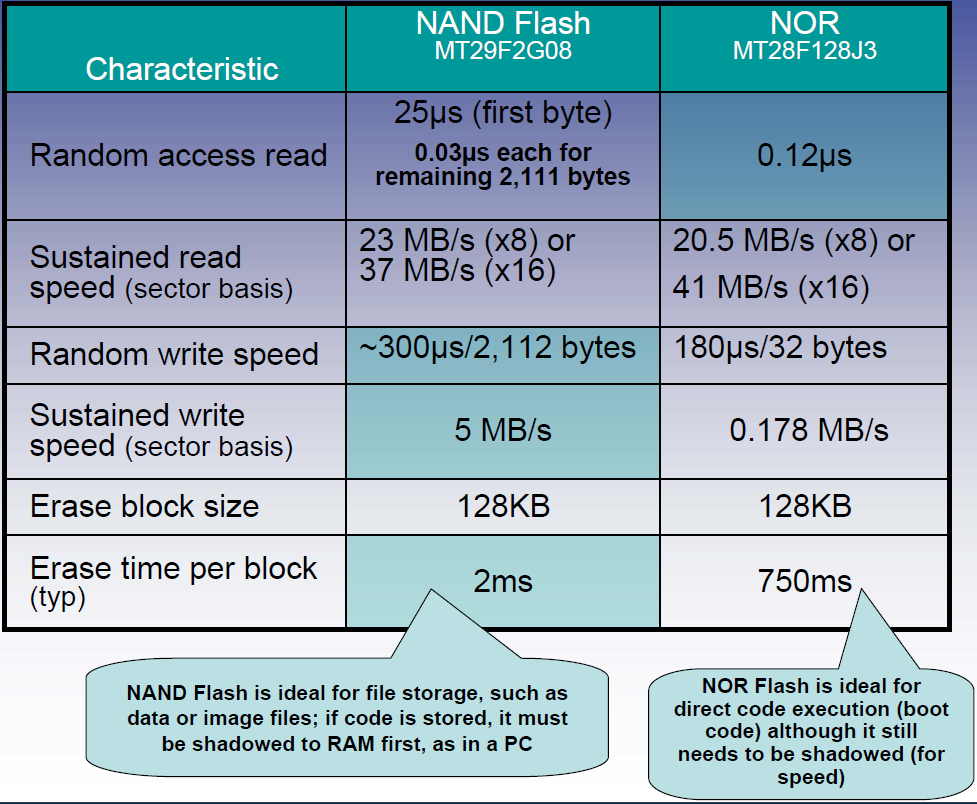
\includegraphics[width=0.6\textwidth]{memorie/jc_numeri}
	\caption{Confronto tra alcune velocità tipiche di NAND e NOR flash}
\end{figure}

\subsection{Interfaccia esterna}
Tipicamente, la NAND flash è gestita da un master, chiamato \textbf{NAND controller}, che, nei microcontrollori di fascia medio-alta, si trova spesso già integrato. 

\subsubsection{Segnali di controllo}
\begin{itemize}
	\item \textbf{Chip Enable} ($\overline{CE}$): seleziona o meno il chip di memoria.
	\item \textbf{Read Enable} e \textbf{Write Enable} ($\overline{RE}$, $\overline{WE}$): segnali di strobe utilizzati per segnalare un ciclo di lettura o scrittura rispettivamente.
	\item \textbf{Address Latch Enable} e \textbf{Command Latch Enable} ($ALE$, $CLE$): servono a segnalare se sul bus si sta mandando un indirizzo, un comando, oppure un dato. In particolare, quando $ALE=1$ e $CLE=0$ su bus è presente un indirizzo, quando $ALE=0$ e $CLE=1$ su bus è presente un comando e quando $ALE=0$ e $CLE=0$ su bus è presente un dato. La configurazione in cui entrambi sono a 1 logico non è definita.
	\item \textbf{Write Protect} ($\overline{WP}$): se asserito, blocca la scrittura nella flash.
	\item \textbf{Ready/Busy} ($R/\overline{BY}$): diretto dalla memoria al controllore, segnala quando la flash è disponibile oppure occupata a svolgere operazioni. 
\end{itemize}
Per lo scambio di dati, il protocollo prevede un bus bidirezionale da 8 bit (16 bit in casi particolari) multiplexato in cui, come detto sopra, passano sia indirizzi, sia comandi, sia dati. Rispetto alla NOR quindi, che invece presenta bus separati per indirizzi e dati e non multiplexati, il numero di piedini è minore, il che garantisce un risparmio notevole.

È previsto, infine, un indirizzo a 40 bit a prescindere dalla dimensione effettiva dell'array di memoria, che permette quindi di indirizzare fino a un massimo di \SI{1}{\tera\byte}. Questo accorgimento permette di mantenere invariata la piedinatura del chip, al fine di ridurre i costi di produzione ai costruttori, evitando di dover specializzare le parti meccaniche o i circuiti stampati per chip di capacità diverse. 

\subsection{Operazioni di base}\label{sec:nand_ops}
Lo schema a blocchi della NAND flash prevede innanzitutto un array di memoria diviso in blocchi a loro volta composti da pagine, che costituiscono l'unità scrivibile elementare della flash. Come nelle SDRAM, spesso ci sono due banchi di memoria (chiamati \textbf{piani}), in modo da poter effettuare due operazioni contemporanee su due pagine appartenenti a diversi blocchi. 

Quindi, è presente un'unità di controllo a cui vengono inviati i comandi sia in lettura che in scrittura. Quindi, a differenza della NOR flash in cui a lettura era effettivamente una lettura dall'array di memoria, qui nessuna operazione agisce direttamente sulle celle di memoria, ma tutte passano dalla FSM interna.

Un secondo elemento fondamentale per le operazioni di una NAND flash è il cosiddetto \textbf{page register}: uno shift register PISO (Parallel In Serial Out), utilizzato per salvare il contenuto di una pagina intera di memoria. Tipicamente esso lavora ad una frequenza intorno ai \SI{30}{\mega\hertz} nel caso di flash asincrone, a causa delle difficoltà progettuali che le unità di controllo asincrone pongono, mentre può arrivare fino a \SI{200}{\mega\hertz} nel caso di flash sincrone.

\begin{figure}[hbtp]
	\centering
	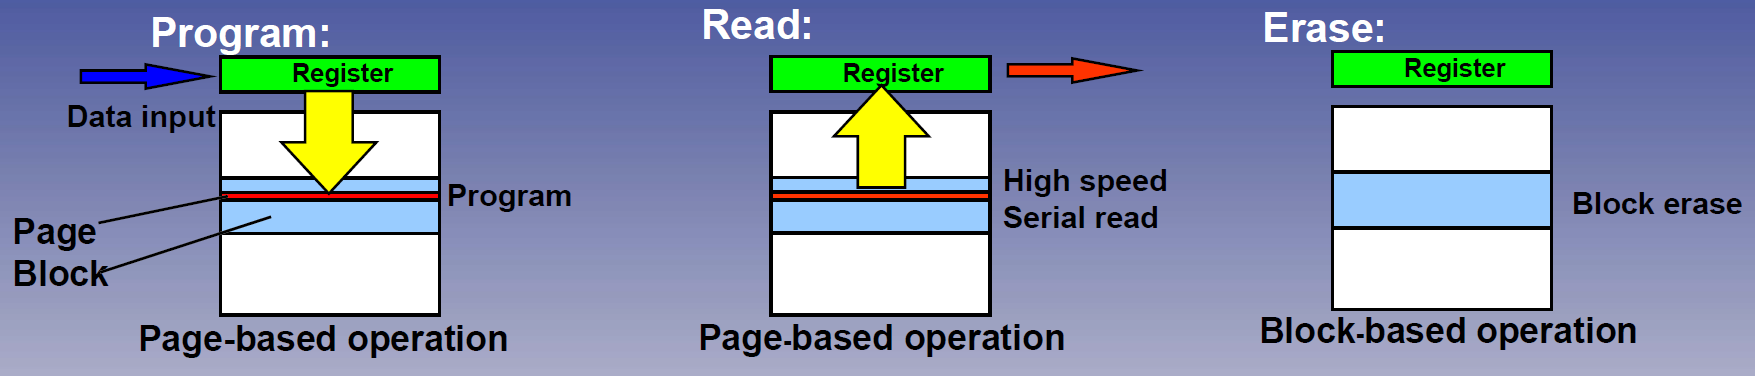
\includegraphics[width=\textwidth]{memorie/jc_operations}
	\caption{Le tre operazioni di base di una NAND flash}
	\label{fig:jc_operations}
\end{figure}

In riferimento alla figura \ref{fig:jc_operations}, quando si effettua un'operazione di lettura, un'intera pagina viene trasferita nel page register in circa \SI{25}{\micro\second} per poi essere serializzata e mandata in uscita.

Il procedimento opposto avviene invece in scrittura, in cui un'intera pagina viene scritta nel page register e poi, con un comando di scrittura, trasferita verso l'array.

In cancellazione, invece, il page register non entra in gioco ed ogni operazione agisce non su una singola pagina, ma su un intero blocco.

Alcuni modelli di NAND flash permettono di eseguire il cosiddetto \textbf{partial page programming}, ovvero la scrittura solamente di una porzione di pagina per volta, tipicamente \SI{512}{\byte}. Il numero di operazioni di scrittura diverse che di possono eseguire su una stessa pagina è sempre specificato nel datasheet. L'uso di tale funzione, prerogativa delle flash SLC (Single Level Cell) trattate finora, è sconsigliata a meno di esigenze particolari.

Per eseguire ogni qualunque operazione, la sequenza di accessi prevede sempre prima la scrittura di un comando seguito da altri 5 cicli in cui si trasferiscono i 40 bit relativi all'indirizzo a cui si vuole operare (figura \ref{fig:jc_access}). Se la memoria è più piccola, i bit di indirizzo non utilizzati vengono posti a 0.

\begin{figure}[hbtp]
	\centering
	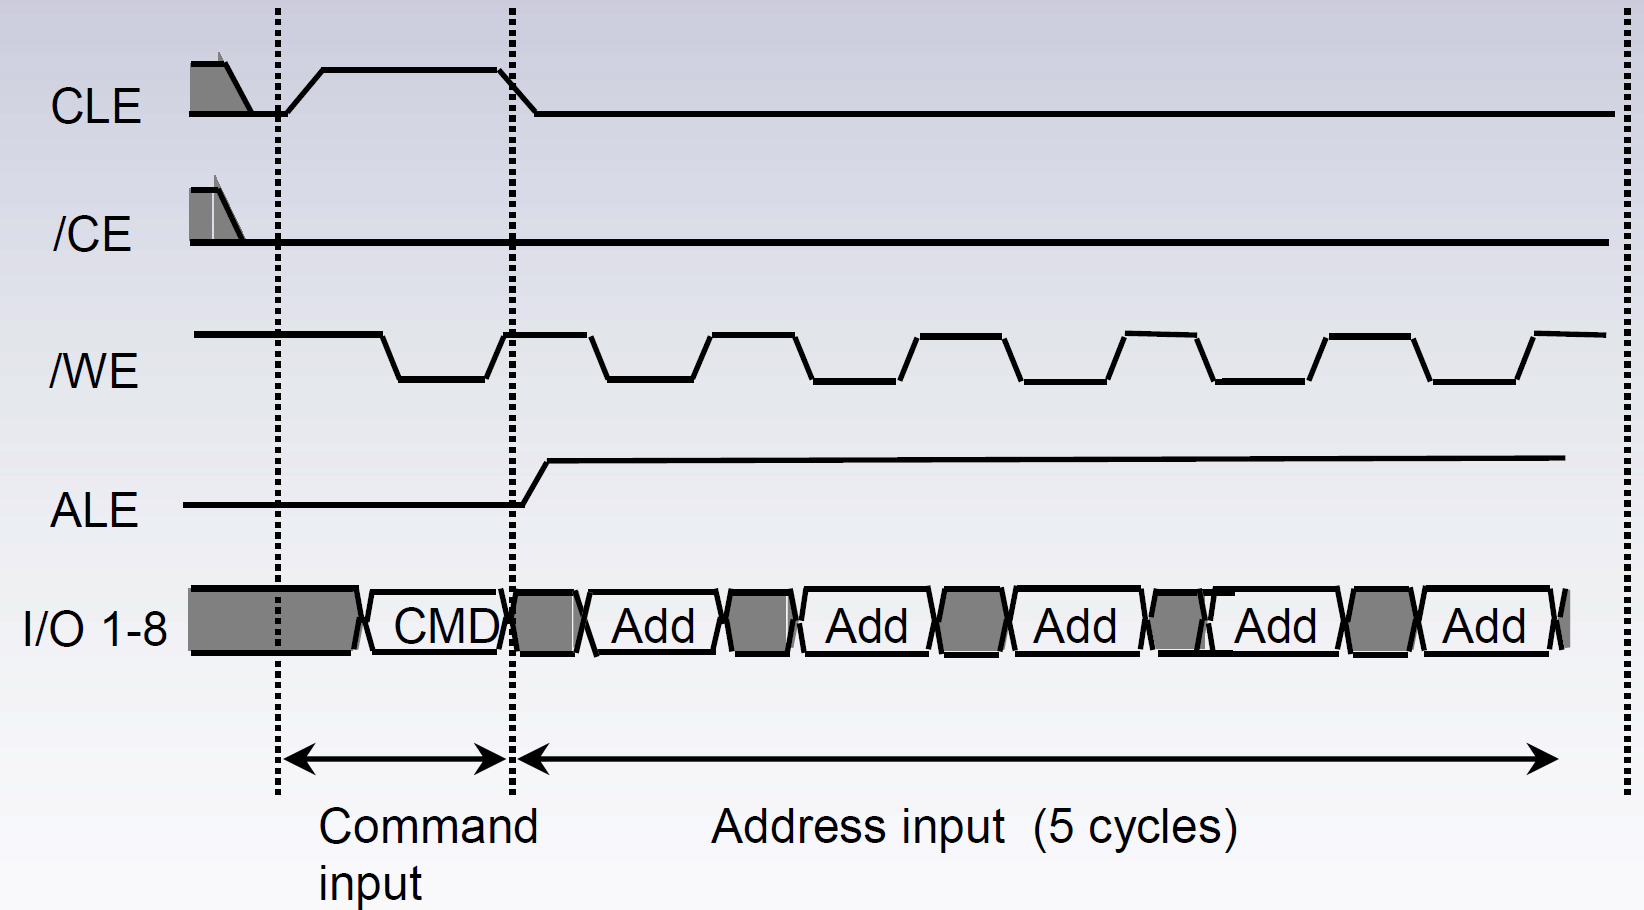
\includegraphics[width=0.6\textwidth]{memorie/jc_access}
	\caption{Sequenza di accesso}
	\label{fig:jc_access}
\end{figure}

Il page register contiene sempre, oltre alle dimensioni di una pagina, dei byte aggiuntivi di correzione degli errori (ECC). Questi possono essere posizionati al fondo dello shift register, oppure inframmezzati alle aree in cui viene salvato l'effettivo payload. In quest'ultimo caso, il vantaggio è poter calcolare i codici di correzione più volte durante lo scorrimento del registro, ma lo svantaggio è avere meno bit di ECC per ogni sezione di dati.
\pagebreak
\begin{tcolorbox}[breakable]
\textbf{ECC, CRC, polinomiali...}\\
Il metodo più semplice per rilevare degli errori consiste nell'inserire un bit aggiuntivo di parità, che indichi se il numero di bit a 1 è pari (parità a 0 logico) o dispari (parità a 1 logico). Così facendo, però, non è possibile rilevare un numero pari di errori o determinare la posizione dei bit errati.

La parità, tuttavia, non è nient'altro che un caso particolarmente semplice di \textbf{Cyclic Redundancy Check} (CRC), ovvero un metodo automatico di individuazione e correzione degli errori basato sulla divisione polinomiale.

Ipotizziamo di avere 32 bit e quindi un dizionario formato da $2^{32}$ parole diverse. Supponiamo di aggiungere altri 6 bit, ma di continuare a codificare soltanto $2^{32}$ parole: in questo modo esisteranno alcune combinazioni di bit proibite ($2^{38}-2^{32}$) che, nel caso vengano lette, indicheranno sicuramente un errore. 

Memorizzando in questi 6 bit il risultato di una divisione tra polinomi opportuni al momento della scrittura e ricalcolando tale risultato ad ogni lettura, si può equivalentemente rilevare un errore in caso di discordanza tra i due valori.

Si può dimostrare che con 6 bit aggiuntivi si possono rilevare tutti gli errori su al massimo 2 bit e che, scegliendo opportunamente la disposizione delle parole proibite all'interno dell'insieme di tutte quelle disponibili, si può fare in modo che cambiando un bit alla volta nella parola letta, solo la modifica del bit effettivamente sbagliato permetta di ottenere una parola tra quelle codificate nel dizionario. In questo modo si può anche capire quali siano i bit sbagliati e di conseguenza correggerli.

Un modo molto semplice di implementare tale algoritmo è fornito da un circuito chiamato \textbf{Linear Feedback Shift Register} (LFSR), che consiste soltanto di uno shift register e due porte XOR.
\end{tcolorbox}

\subsection{Multi Level Cell (MLC)}
Le prime memorie flash sviluppate, sia NAND che NOR contenevano dei transistor a gate flottante che potevano memorizzare un 1 logico in funzione della presenza o meno di carica nel gate. Successivamente, si è deciso di operare una programmazione più raffinata, introducendo quattro livelli diversi di carica nel gate, al fine di memorizzare 2 bit di informazione su ogni singolo transistor. Questa tipologia di memoria flash si chiama \textbf{Multi Level Cell} (MLC) e permette, senza modifiche fisiche al dispositivo, di raddoppiarne la capacità, dimezzando così il costo per bit. Tale tecnologia si trova applicata soprattutto alle NAND flash, che vengono utilizzate come dispositivi di storage, mentre è rara nelle NOR flash che vengono impiegate specialmente in dimensioni ridotte e quindi ne beneficiano.

\begin{figure}[hbtp]
	\centering
	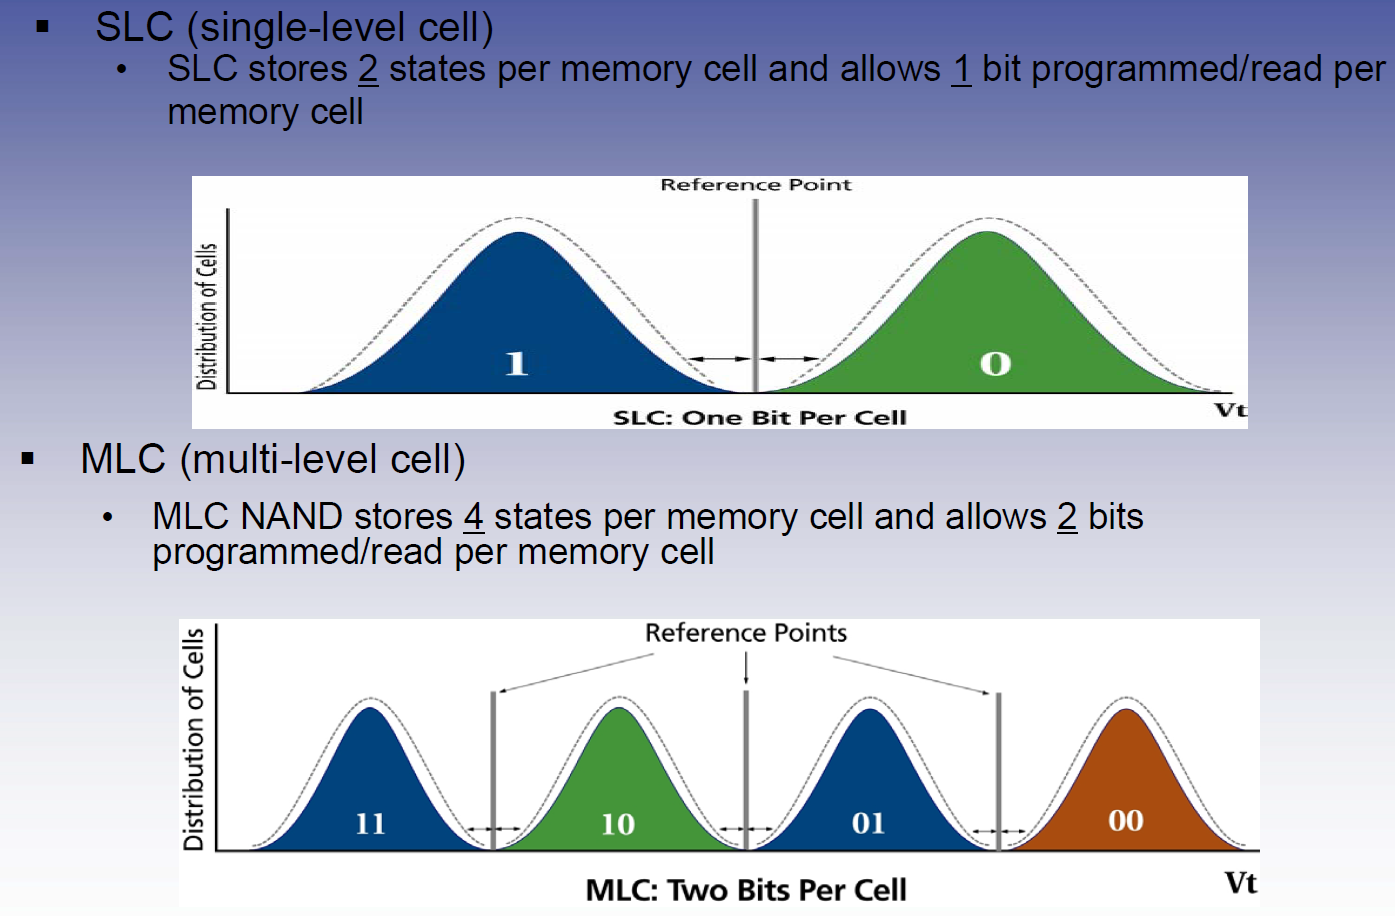
\includegraphics[width=0.7\textwidth]{memorie/jc_slc_mlc_gauss}
	\caption{Confronto tra le distribuzioni della carica nelle celle, in funzione della tensione.}
	\label{fig:jc_slc_mlc_gauss}
\end{figure}

Nelle flash SLC, per verificare se una cella memorizza uno 0 oppure un 1, basta applicare sul gate una singola tensione, ovvero quella di alimentazione, chiamata \emph{reference point} nei grafici di figura \ref{fig:jc_slc_mlc_gauss}. Dal momento che la programmazione è un processo stocastico, tali grafici mostrano una distribuzione gaussiana delle tensioni di soglia, piuttosto che un singolo punto sull'asse orizzontale.

Nelle MLC, invece, dividendo lo stesso asse in quattro intervalli, risulta evidente come ognuno di essi diventi più stretto e come servano tre diversi punti di riferimento per verificare quale combinazione sia memorizzata. Come conseguenza, la precisione con cui si inseriscono le cariche nel gate flottante deve essere maggiore e perciò l'algoritmo che si occupa della scrittura sarà ragionevolmente più lento. Ne consegue una riduzione delle prestazioni rispetto alle memorie SLC.

Inoltre, data questa compressione orizzontale, è anche evidente come l'affidabilità di una flash MLC sia minore rispetto a quella di una SLC, perché anche una piccola variazione della tensione di soglia può portare ad un errore nella coppia di bit memorizzata.

Tali differenze portano i due tipi di memoria flash ad avere target di mercato diversi:
\begin{itemize}
	\item Le flash SLC sono utilizzate nelle memory card ad alte prestazioni, negli SSD di fascia alta e nelle memorie interne degli smartphone. In generale, in tutte le applicazioni in cui alte prestazioni e alta affidabilità siano necessari. Ovvero, le applicazioni \emph{industrial}, in cui un malfunzionamento può generare danno economico.
	\item Le MLC, invece, sono presenti ad esempio nei media player, nelle chiavette USB e nelle memory card di fascia medio-bassa. In generale, in tutte le applicazioni \emph{consumer} in cui il basso costo è più importante dell'alta affidabilità o delle elevate prestazioni.
\end{itemize}

\begin{figure}[hbtp]
	\centering
	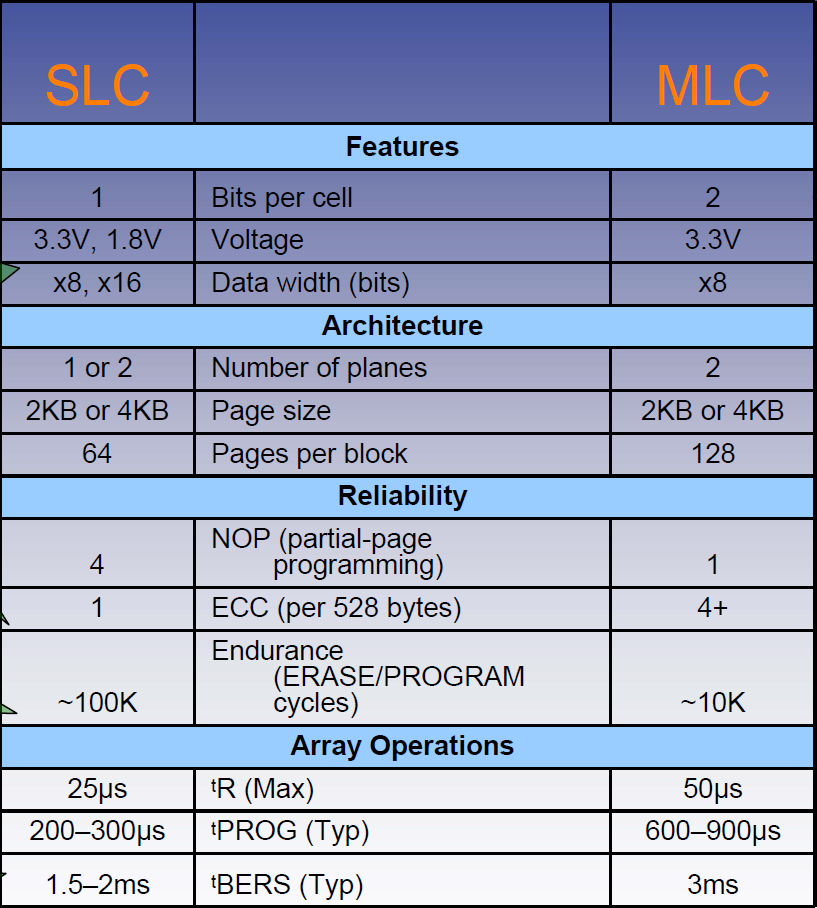
\includegraphics[width=0.6\textwidth]{memorie/jc_slc_mlc_numeri}
	\caption{Alcuni valori tipici di flash SLC e MLC}
	\label{fig:jc_slc_mlc_numeri}
\end{figure}

In figura \ref{fig:jc_slc_mlc_numeri} è presente un confronto quantitativo tra le due tipologie di memoria flash. Si nota innanzitutto che le SLC possono lavorare correttamente anche a tensioni basse fino a \SI{1.8}{\volt}, dal momento che due soli intervalli di decisione non richiedono un campo di tensioni ampio su cui discriminare. D'altra parte, le MLC vengono offerte principalmente con tensione di alimentazione di \SI{3.3}{\volt} e solo ultimamente si trovano alcuni modelli alimentati a tensione più bassa.

Solo le SLC offrono la possibilità di fare il partial page programming e richiedono un solo bit di ECC, contro i 4 delle flash MLC, proprio perché la loro affidabilità è intrinsecamente maggiore. Questo è un duplice vantaggio per le SLC in quanto la maggior parte dei NAND controller integrati nei microcontrollori supporta nativamente 1 bit di ECC.

In termini di endurance, le MLC possono sopportare un numero di cicli lettura/scrittura un ordine di grandezza inferiore rispetto alle SLC, prima che i difetti creatisi nel reticolo danneggino permanentemente una cella.

Anche in termini di tempistiche, si noti come nelle MLC i tempi di lettura, programmazione e cancellazione di un blocco siano dalle 2 alle 3 volte superiori rispetto a quelli delle SLC.

\subsection{Prestazioni}
Quando le NAND sono state introdotte sul mercato, inizialmente le loro prestazioni erano inferiori a quelle delle NOR, ma in poco tempo sono migliorate fino a superarle. Per capire dove ancora ci sia margine di miglioramento, tuttavia, bisogna identificare quali siano i colli di bottiglia per le prestazioni. 

\subsubsection{Lettura}
In lettura, per trasferire una pagina dall'array di memoria al page register servono circa \SI{25}{\micro\second} per le SLC o \SI{50}{\micro\second} per le MLC. Per shiftare poi i dati in uscita, sono necessari invece \SI{20}{\nano\second} per ogni byte della pagina, ovvero \SI{42}{\micro\second} nel caso di pagine da \SI{2}{\kilo\byte} o \SI{86}{\micro\second} nel caso di pagine da \SI{4}{\kilo\byte}. 

In generale quindi, il tempo di I/O è dalle 2 alle 4 volte superiore al tempo di trasferimento dall'array, perciò tale risulta essere il collo di bottiglia in lettura. Ne consegue che rendere più veloce l'array di memoria è del tutto inutile. Il problema non è di immediata soluzione, perché, come già accennato al paragrafo \ref{sec:nand_ops}, la frequenza di lavoro dell'interfaccia di I/O non può scalare facilmente in quanto asincrona. 

\begin{figure}[hbtp]
	\centering
	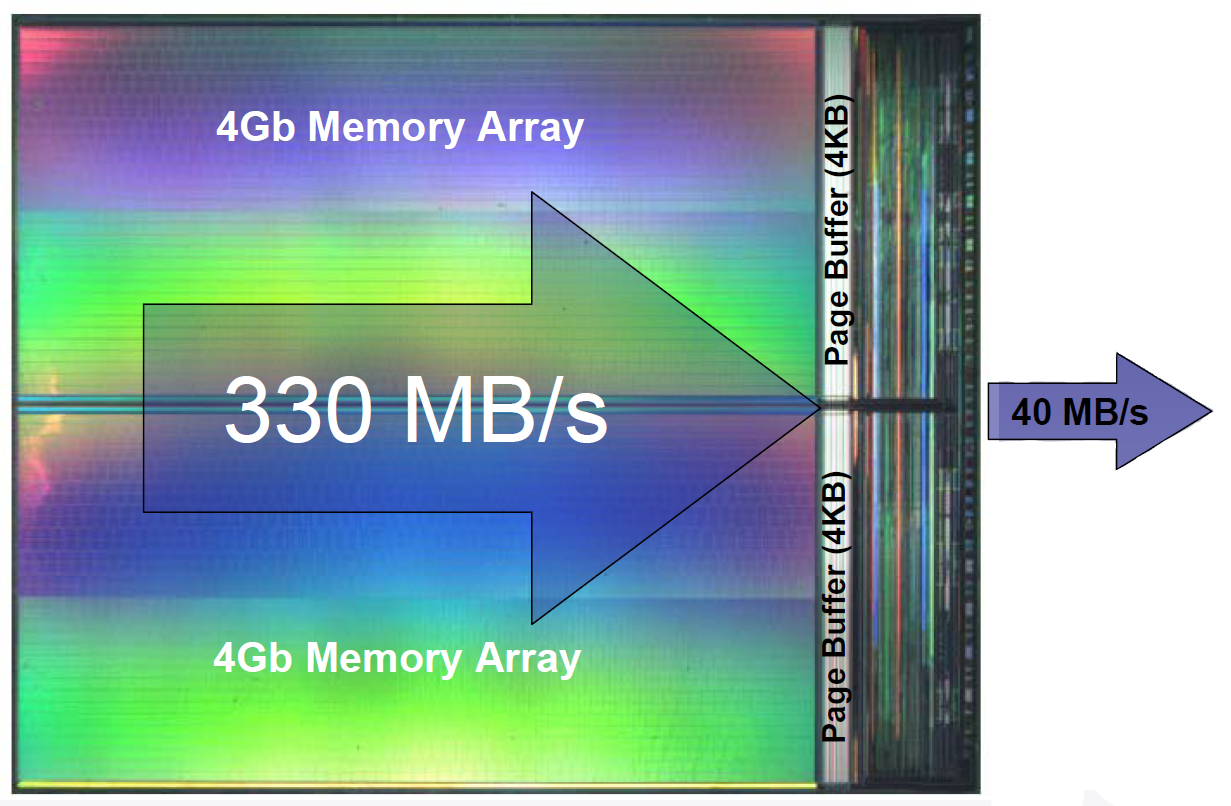
\includegraphics[width=0.5\textwidth]{memorie/jc_read_bn}
	\caption{Asimmetria tra le bande in lettura}
	\label{fig:jc_read_bn}
\end{figure}

La figura \ref{fig:jc_read_bn} illustra la grande asimmetria che si rileva tra la banda del trasferimento dall'array e quella del bus, durante una lettura. Le prestazioni dell'array sono sfruttate soltanto per il 12\% delle loro potenzialità.

Per fare un confronto, una situazione simile si ha con l'interfaccia SATA, comunemente utilizzata nei PC, che può sostenere \SI{600}{\mega\byte\per\second}, mentre i supporti magnetici ad essa connessi arrivano a malapena a \SI{50}{\mega\byte\per\second}. 

\subsubsection{Scrittura}
Per l'operazione di scrittura, invece, la situazione è diametralmente opposta, con l'array di memoria che costituisce l'effettivo collo di bottiglia. Infatti, mentre il bus di I/O funziona alla stessa frequenza indipendentemente dall'operazione effettuata, la scrittura nella flash è estremamente più lenta rispetto alla lettura, il che porta ad una drastica diminuzione della banda dell'array. 

Tale situazione, illustrata in figura \ref{fig:jc_write_bn}, è comunque meno grave della precedente in quanto l'asimmetria tra i valori e minore (si sfrutta l'83\% della banda del bus)e perché le scritture sono molto meno frequenti delle letture in una flash.

\begin{figure}[hbtp]
	\centering
	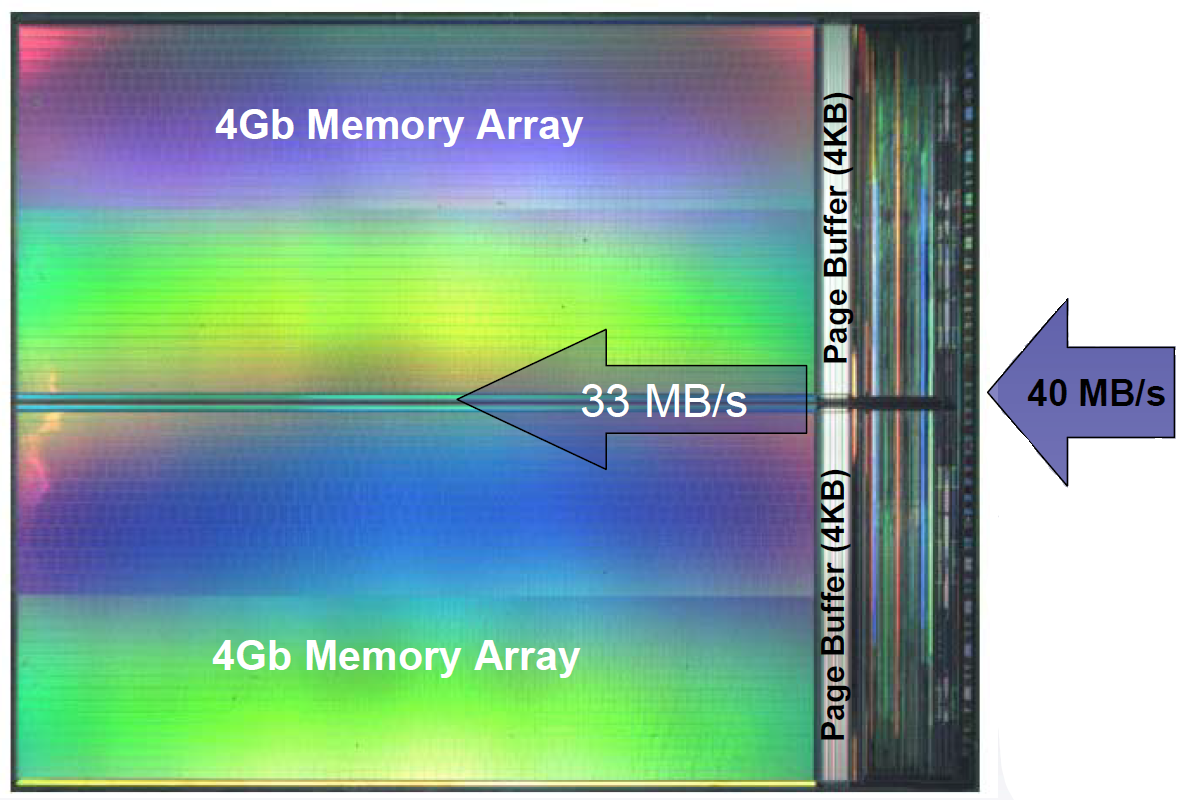
\includegraphics[width=0.5\textwidth]{memorie/jc_write_bn}
	\caption{Asimmetria tra le bande in scrittura}
	\label{fig:jc_write_bn}
\end{figure}

\subsection{ONFI e NAND flash ad alte prestazioni}
L'Open NAND Flash Interface (ONFI) un'associazione che riunisce i produttori, i consumatori e i \emph{technology enabler} (cioè coloro che trovano delle applicazioni per gli oggetti prodotti) delle NAND flash. Il suo scopo è la standardizzazione dell'interfaccia delle NAND flash, al fine di garantire l'interoperabilità tra le memorie di costruttori diversi, in modo simile al lavoro svolto dalla CFI nelle NOR flash.

Senza uno standard, infatti, numerosi fattori potrebbero non essere consistenti tra diversi modelli il che risulterebbe in una penalizzazione generale per il mercato. Ad esempio, potrebbero non essere univoci l'identificazione del dispositivo, la modalità di indirizzamento, la struttura dell'array,il set di comandi, il timing, il numero di bit di ECC, i blocchi marcati alla fabbrica come non funzionanti ecc.

Tutte queste informazioni vengono memorizzate in una pagina dedicata all'interno della flash e possono essere lette dal software del NAND controller all'avvio per prende decisioni atte a sfruttare al meglio le caratteristiche del dispositivo presente nel sistema.

\subsubsection{ONFI 1.0}
L'interfaccia che è stata esaminata finora è chiamata ONFI 1.0. Essa ha permesso di rendere più agevole il progetto dei NAND controller, mettendo a disposizione una modalità semplice e standard di verifica delle caratteristiche del chip. È bene specificare che una flash può funzionare anche senza un apposito controllore tuttavia, in questo caso non si riuscirebbero a sfruttarne appieno le potenzialità.

ONFI 1.0 ha anche introdotto i cosiddetti \emph{timing mode}, ovvero dei protocollo per la temporizzazione delle NAND flash. Il più alto tra questi (timing mode 5) permette cicli di lettura e scrittura fino a \SI{50}{\nano\second}. 

\subsubsection{ONFI 2.0}
Lo standard ONFI 2.0 è nato con l'obiettivo di definire un'interfaccia per le NAND flash ad alte prestazioni di nuova generazione. La prima prerogativa è stata il mantenimento della compatibilità all'indietro tra i segnali di interfaccia. In questo modo, il NAND controller all'avvio può eseguire una procedura di identificazione del dispositivo a bassa velocità in modo del tutto asincrono, utilizzando i segnali da sempre disponibili in tali memorie, e quindi, nel caso in cui si riconosca un chip che supporta ONFI 2.0, può specializzare il suo funzionamento per sfruttarlo appieno.

In secondo luogo, si sono introdotti degli accorgimenti per migliorare il throughput dell'interfaccia di I/O, cercando di mantenere del margine di crescita per il futuro. Le novità introdotte sono le seguenti:
\begin{itemize}
\item Si è introdotto un protocollo sincrono per la trasmissione dei dati, basato su un segnale DQS, del tutto simile a quello utilizzato nelle SDRAM (cfr. datasheet \ref{ds:ddr3}). Esso è un segnale di strobe sempre sincrono con la sorgente, ovvero, viene inviato dalla memoria in lettura, ma dal NAND controller in scrittura.
\item I segnali di strobe $\overline{RE}$ e $\overline{WE}$ sono stati sostituiti da un segnale di clock e un $R/\overline{W}$ che indica quando si vuole effettuare una lettura o una scrittura. Si noti che di questi segnali è cambiata solo la semantica, le connessioni sono rimaste identiche per le considerazioni fatte in precedenza sulla compatibilità. In questo modo, all'avvio, il NAND controller si interfaccia dapprima in modo asincrono e quindi, se rileva un chip compatibile, cambia il significato di questi due segnali e inizia a comunicare in modo sincrono (figura \ref{fig:jc_sync_async}).
\item Si è reso il protocollo di scambio dati DDR, anche qui in modo simile alle SDRAM.
\item Dal momento che il collo di bottiglia delle prestazioni è esclusivamente il trasferimento dei dati, tale nuovo protocollo è stato implementato solo per essere usato durante lettura/scrittura di dati e non di indirizzi. Infatti, gli indirizzi vengono scritti in modalità SDR e campionati sul fronte del clock (e non su DQS) (figura \ref{fig:jc_onfi2_timing}).
\item Per ridurre il consumo di potenza dovuto alla maggiore velocità, si è cercato di minimizzare la capacità dei pin del package, il che ha portato alla scelta di un package BGA che limita le capacità parassite in quanto ha i piedini di area minore sul mercato (\SI{0.25}{\milli\meter^2}). Grazie alla densità di pin in questo tipo di package, come ulteriore valore aggiunto è nata la possibilità di estendere il bus da 8 a 16 bit, permettendo di mettere all'interno dello stesso package due chip di memoria, o di produrre un singolo chip con parallelismo doppio.
\item Per lo stesso motivo, si è diminuita la tensione di alimentazione dell'interfaccia di I/O, mentre quella del core è rimasta invariata dato che il consumo di potenza non è localizzato nell'array. Di conseguenza, il NAND controller deve disporre al suo interno di un alimentatore programmabile, tipicamente un buck converter.
\end{itemize}

\begin{figure}[hbtp]
	\centering
	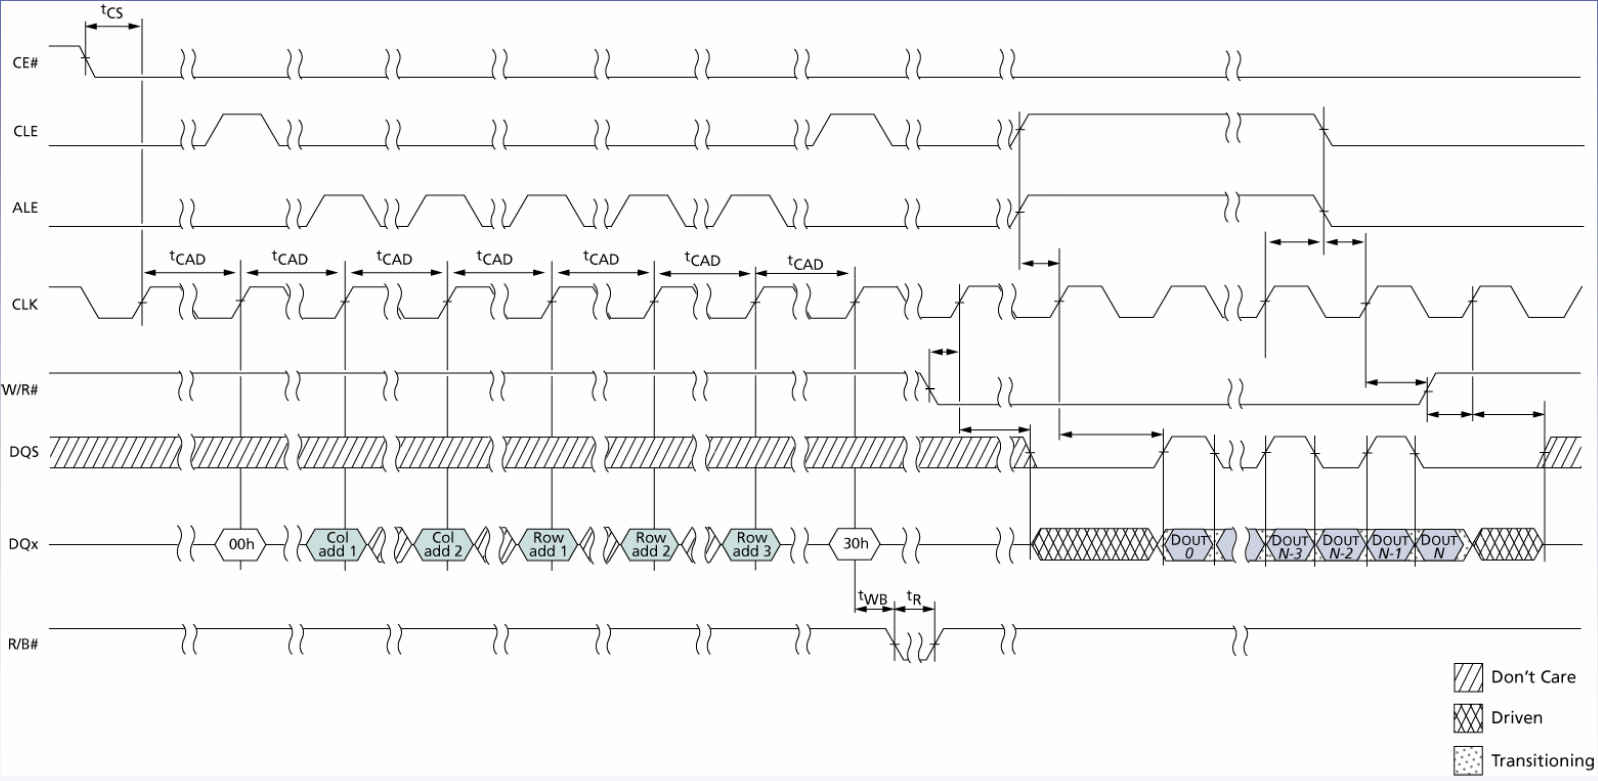
\includegraphics[width=\textwidth]{memorie/jc_onfi2_timing}
	\caption{Timing di indirizzi e dati per lo standard ONFI 2.0}
	\label{fig:jc_onfi2_timing}
\end{figure}

\begin{figure}[hbtp]
	\centering
	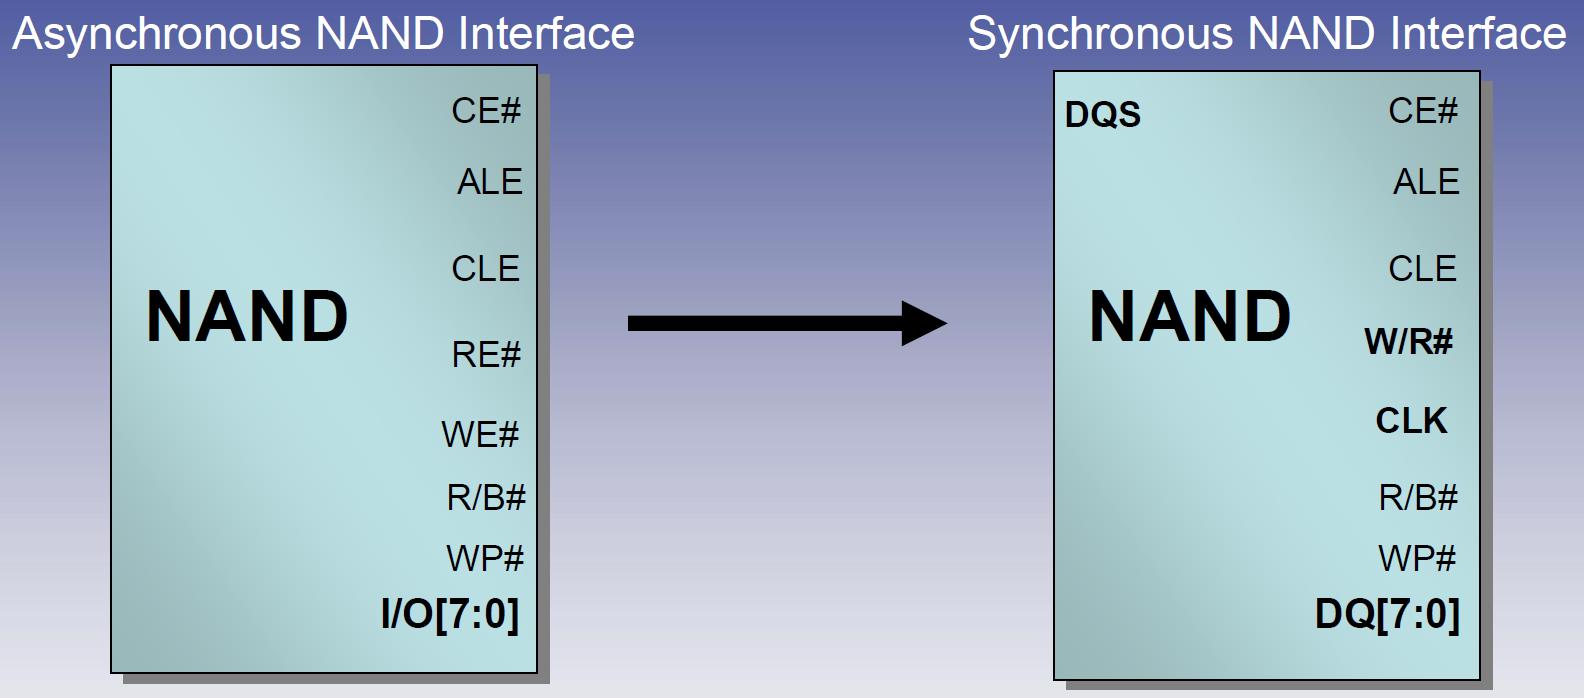
\includegraphics[width=0.7\textwidth]{memorie/jc_sync_async}
	\caption{Passaggio dall'interfaccia asincrona a quella sincrona}
	\label{fig:jc_sync_async}
\end{figure}

\begin{figure}[hbtp]
	\centering
	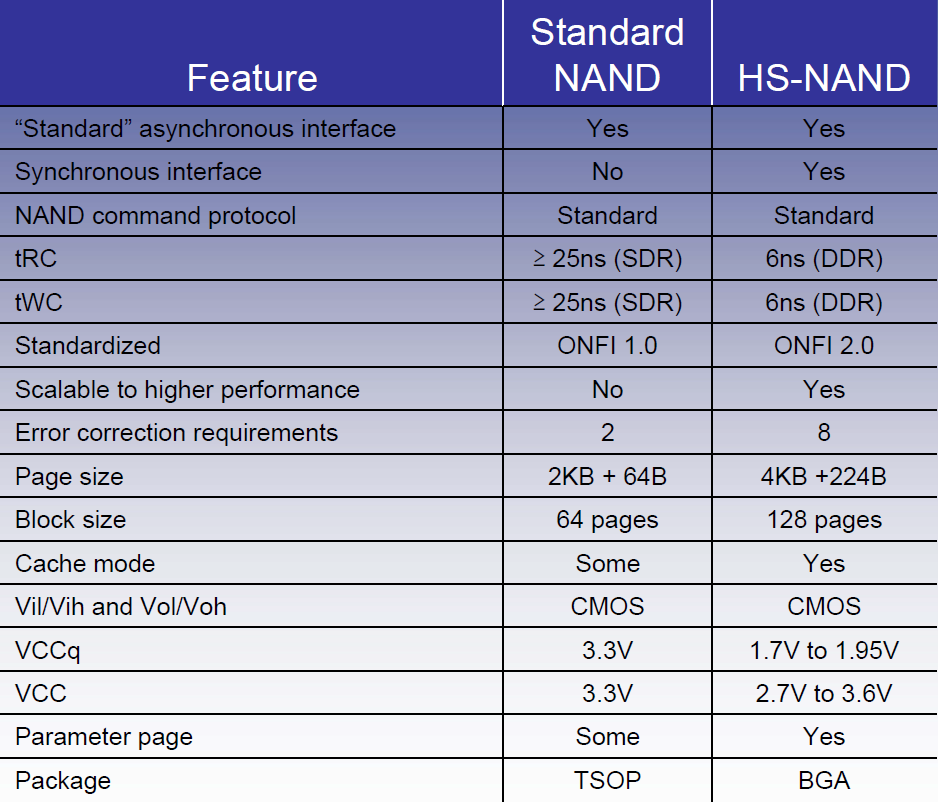
\includegraphics[width=0.6\textwidth]{memorie/jc_onfi2_table}
	\caption{Tabella riepilogativa di confronto tra una NAND flash standard e ad alte prestazioni}
	\label{fig:jc_onfi2_table}
\end{figure}

Dalla tabella riepilogativa di figura \ref{fig:jc_onfi2_table}, si noti che un aspetto negativo di tale nuova interfaccia è il numero più alto di bit di ECC necessari, a causa dell'aumento della possibilità di errore provocato dalla maggiore velocità operativa.

Il risultato netto di queste modifiche sull'interfaccia delle NAND flash è stato un aumento dello sfruttamento della banda dell'array di memoria di oltre il 250\% in lettura.

L'avvento di questo nuovo standard intorno al 2006-2007 ha segnato un passaggio importante nella storia delle memorie flash, perché per la prima volta le loro prestazioni sono diventate comparabili con quelle dei tradizionali HDD meccanici. Questo ha provocato un passaggio di testimone, con gli HDD che da allora vengono impiegati soltanto dove servano capacità di archiviazione ancora non raggiunte con le memorie flash.

\subsection{Cause di errore}
Le NAND flash hanno, dal punto di vista tecnologico, delle modalità di errore diverse dalle NOR flash. Le quattro cause più comuni di errore e le loro motivazioni sono presentate di seguito.

\subsubsection{Program disturb}
\begin{figure}[hbtp]
	\centering
	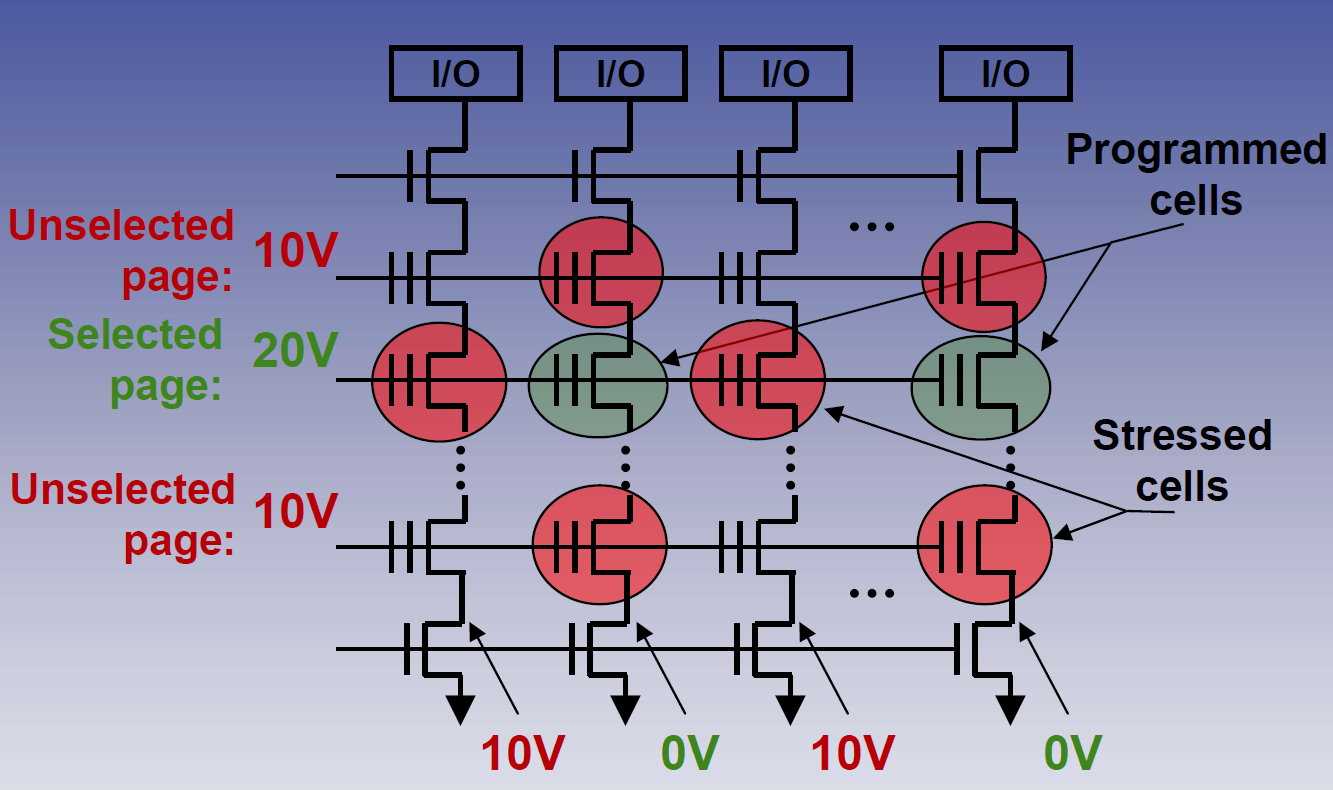
\includegraphics[width=0.6\textwidth]{memorie/jc_program_disturb}
	\caption{Programmazione di una pagina}
	\label{fig:jc_program_disturb}
\end{figure}
In fase di programmazione (figura \ref{fig:jc_program_disturb}), si applica una tensione elevata (as esempio \SI{20}{\volt}) sui gate dei MOS appartenenti alla pagina selezionata, ma è necessario applicare tensione (più bassa, ad esempio\SI{10}{\volt}) anche ai gate di tutti i transistor circostanti in modo da poter raggiungere elettricamente quelli delle celle da programmare effettivamente. 
Quindi, le bitline di tali celle vengono messe a massa, mentre le altre a \SI{10}{\volt} anch'esse, ad esempio.

Dal momento che l'operazione di programmazione è un processo statistico che dipende dalla differenza di potenziale tra gate e canale di ogni singolo MOS, il risultato è che: 
\begin{itemize}
\item Le celle della pagina selezionata che dovevano essere programmate lo saranno sicuramente in quanto tale differenza di potenziale è pari a \SI{20}{\volt}.
\item I transistor delle pagine circostanti collocati sulle bitline a \SI{10}{\volt} non verranno programmati in quanto non cade tensione tra gate e canale.
\item Le celle della pagina selezionata che NON dovevano essere programmate e quelle delle pagine non selezionate in cui però la bitline è a massa potrebbero essere debolmente programmate a causa di elettroni che finiscono nel gate flottante, dal momento che tra gate e canale cade una tensione pari a \SI{10}{\volt}.
\end{itemize}
Questa programmazione non desiderata, chiamata appunto \textbf{program disturb}, non è un danno fisico, in quanto la cancellazione delle celle che ne vengono interessate ripristina la situazione loro originaria. Grazie ai bit di ECC, questa probabilità di errore non è un problema. 

Questo è anche il motivo per cui è sconsigliato effettuare operazioni di partial page programming: programmando più volte la stessa pagina, tale disturbo aumenta notevolmente nelle celle vicine. 

\subsubsection{Read disturb}
\begin{figure}[hbtp]
	\centering
	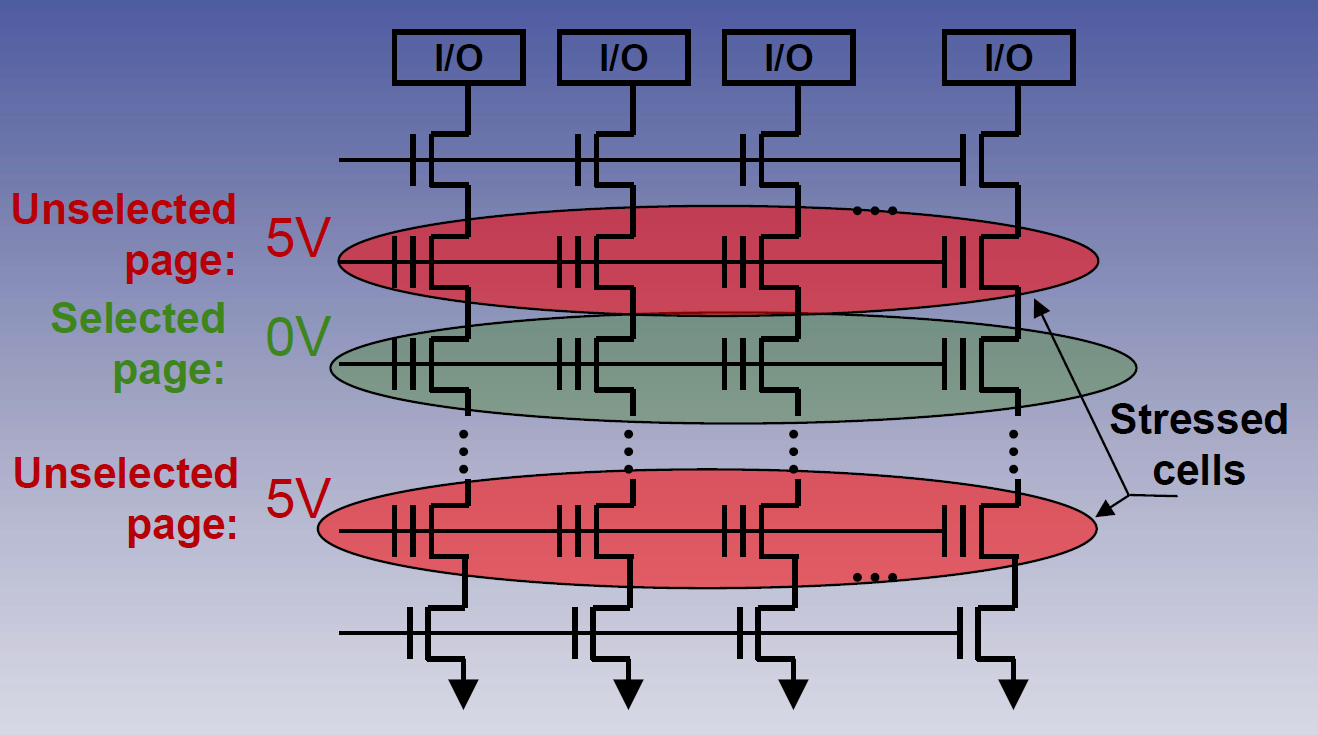
\includegraphics[width=0.6\textwidth]{memorie/jc_read_disturb}
	\caption{Lettura di una pagina}
	\label{fig:jc_read_disturb}
\end{figure}
Un problema simile si ritrova nella fase di lettura (figura \ref{fig:jc_read_disturb}). Per poter accedere ad una pagina, quelle adiacenti sono sottoposte ad una tensione che genera lo stesso effetto di debole programmazione. Anche in questo caso il danno è reversibile con una cancellazione e i suoi effetti vengono mitigati grazie alla ECC.

Questo però è un problema ben più grave del precedente perché, dal momento che le letture sono molte (molte più delle scritture), significa che la lettura può essere distruttiva. 

Per limitare questo disturbo, è utile fare una sorta di refresh periodico, riscrivendo la pagina ogni tot letture. Una regola generale stabilisce tale numero intorno al milione di letture per le flash SLC e, come prevedibile, 10 volte meno per le MLC.

\subsubsection{Data retention}
\begin{figure}[hbtp]
	\centering
	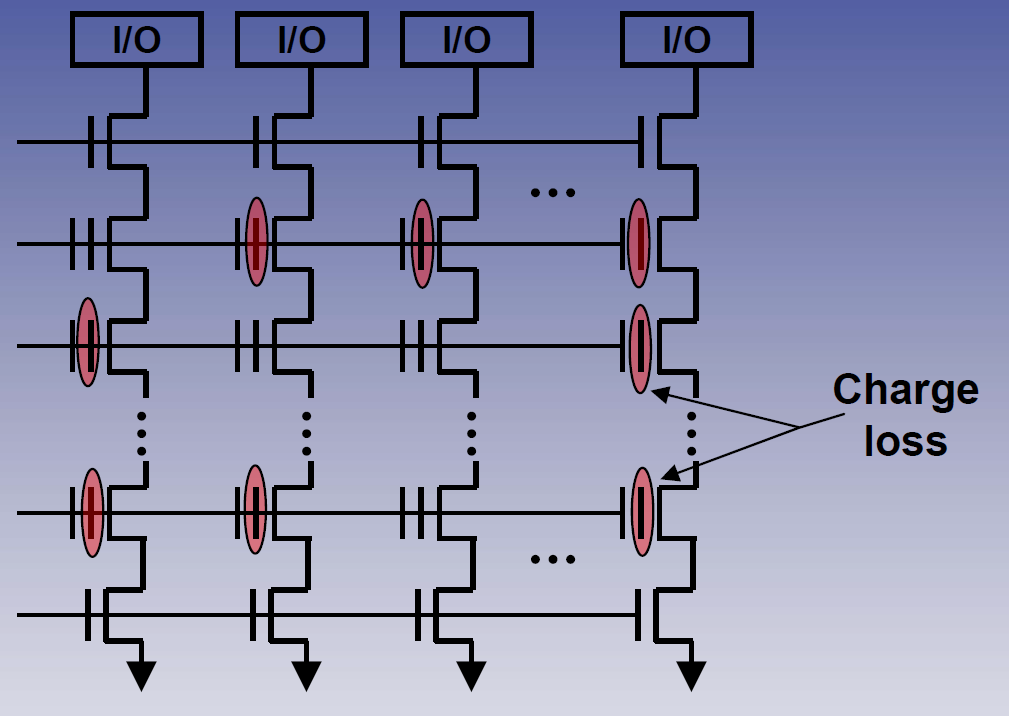
\includegraphics[width=0.6\textwidth]{memorie/jc_data_retention}
	\caption{Perdite dai floating gate}
	\label{fig:jc_data_retention}
\end{figure}
Con le geometri più piccole delle NAND flash rispetto alle NOR, c'è una probabilità non nulla che gli elettroni escano dal floating gate (figura \ref{fig:jc_data_retention}). Questo provoca una deriva della tensione di soglia verso un valore di riposo. Anche questo tipo di errore può essere risolto efficacemente tramite una cancellazione del blocco.

\subsubsection{Endurance}
\begin{figure}[hbtp]
	\centering
	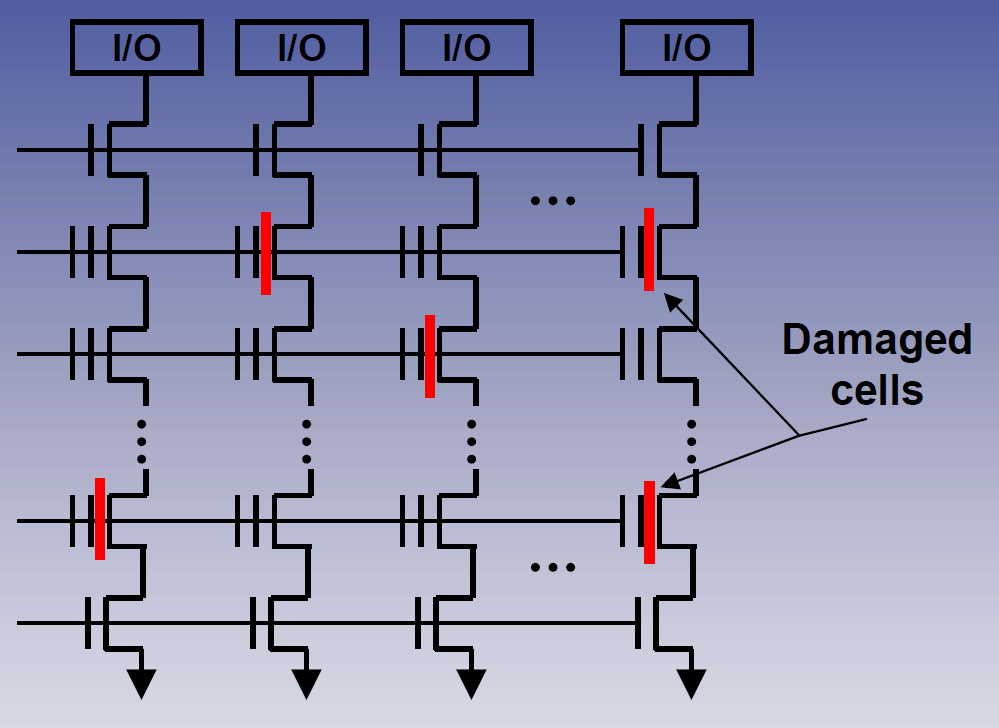
\includegraphics[width=0.6\textwidth]{memorie/jc_endurance}
	\caption{Celle danneggiate a causa del wearing}
	\label{fig:jc_endurance}
\end{figure}
A causa di troppi cicli di lettura/scrittura, il reticolo cristallino delle celle può danneggiarsi e formare livelli trappola che catturano elettroni, con il risultato che tali celle non possono più essere utilizzate. Questa tipologia di errore, detta \textbf{endurance}, è l'unico danno fisico non recuperabile con una cancellazione. 

Per massimizzare la durata della flash di usano algoritmi di \textbf{wear-leveling} che distribuiscano le scritture nelle varie pagine: il microcontrollore fa una mappatura tra i blocchi logici e i blocchi fisici, variandola nel tempo quando rileva che un determinato blocco è stato scritto troppe volte più degli altri. Da un punto di vista computazionale questa è un'operazione onerosa, infatti un SSD da 500 GB attuale di livello industrial può avere all'interno fino a tre processori che lavorano a 1 GHz, dedicati alla gestione di questi algoritmi oltre alle letture, scritture e ECC.

\subsection{Bit di ECC}
\begin{figure}[hbtp]
	\centering
	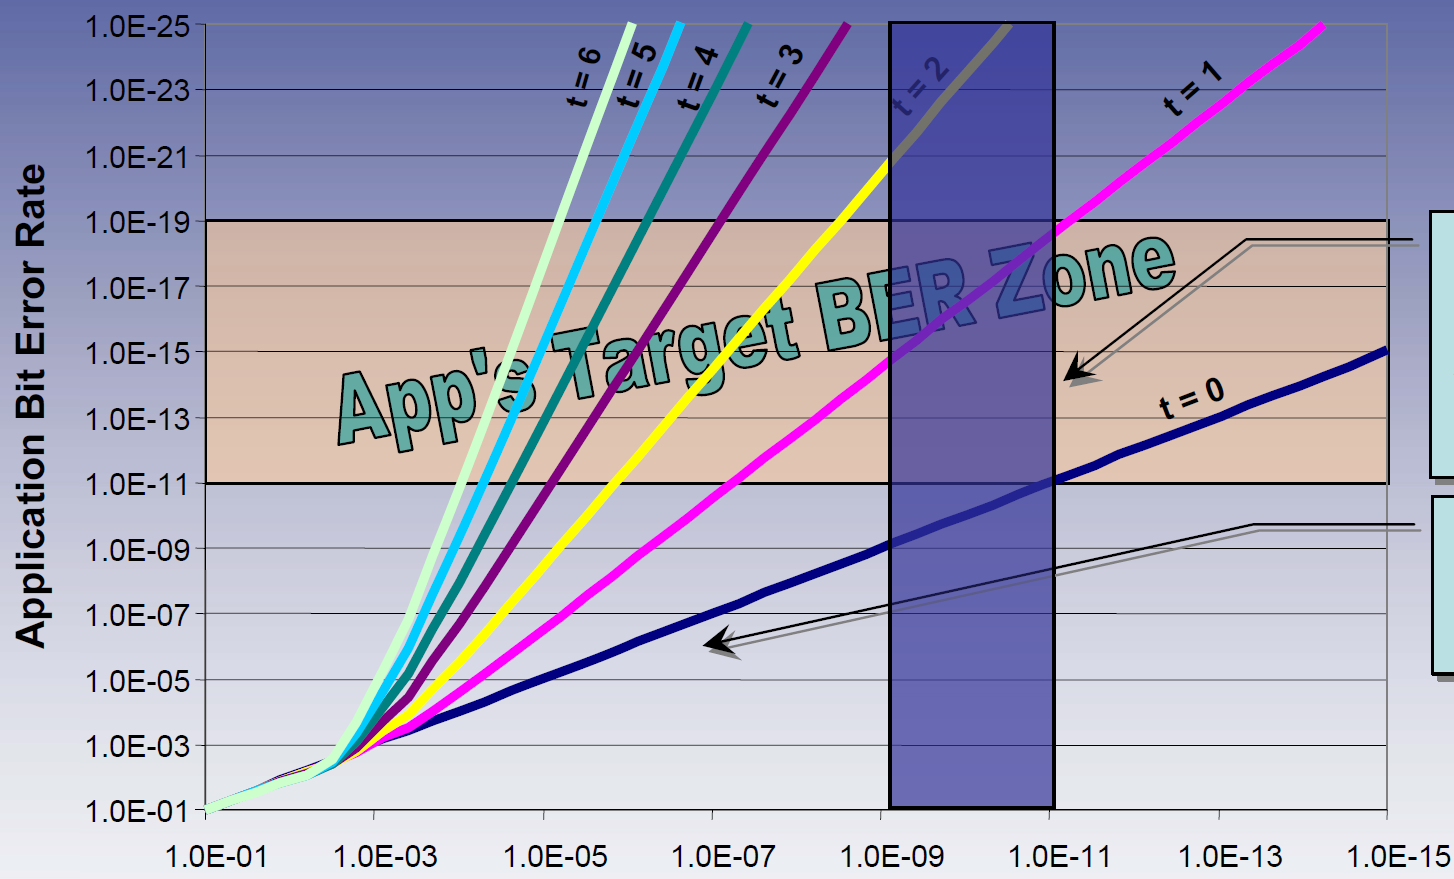
\includegraphics[width=0.7\textwidth]{memorie/jc_ber}
	\caption{BER dell'applicazione in funzione di quello della flash}
	\label{fig:jc_ber}
\end{figure}
Per capire quanti bit di ECC siano necessari, in fase di progetto del sistema, bisogna innanzitutto determinare quale sia la probabilità di errore (\textbf{Bit Error Rate}, BER) accettabile per l'applicazione in esame, ovvero stimare quanto sia rischioso un malfunzionamento.

Quindi, un grafico come quello in figura \ref{fig:jc_ber} può essere utile per stimare il numero di bit di ECC richiesti, conoscendo il BER tipico delle flash in commercio. In figura, il parametro $t$ indica il numero di bit di ECC ogni 512 byte di memoria: con $t=0$, ovviamente, il BER della memoria corrisponde a quello dell'applicazione e non si ha nessun vantaggio, ma già con $t=1$, si ottiene un miglioramento di 6 ordini di grandezza rispetto al BER intrinseco della flash.

\subsection{eMMC}
L'evoluzione della NAND flash per le applicazioni embedded ha portato all'introduzione sul mercato di una NAND flash con un controller integrato in un unico package BGA. Questo standard è chiamato Embedded MMC (eMMC) in quanto il controller utilizzato è lo stesso delle schede di memoria MMC. Tale soluzione offre un'alternativa di storage a basso costo, soprattutto nei dispositivi portatili, rispetto ai tradizionali SSD, garantendo comunque prestazioni confrontabili con essi.
\begin{figure}[hbtp]
	\centering
	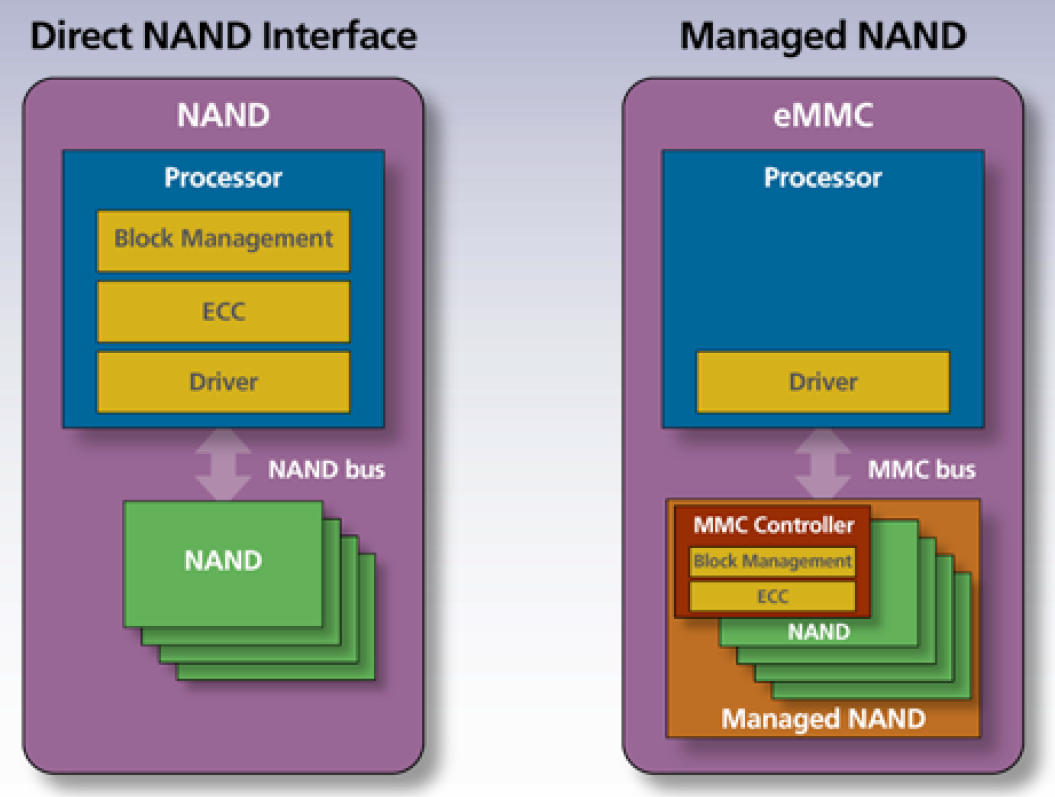
\includegraphics[width=0.4\textwidth]{memorie/jc_emmc}
	\caption{Confronto tra interfaccia NAND flash tradizionale e eMMC}
\end{figure}

\chapter{Sistema di memoria}
La cache e la memoria virtuale una volta erano importanti solo in sistemi dalla potenza di calcolo elevata, ma oggi sempre più spesso è rilevante anche nel mondo dei sistemi embedded, infatti la cache si trova anche in alcuni microcontrollori da almeno 16 bit e la memoria virtuale in alcuni a 32 bit. Ad esempio, i modelli della famiglia Kinetis di NXP o gli STM32 della ST possiedono queste caratteristiche.


Il sistema di memoria tipicamente è composto da una memoria principale (RAM), veloce, costosa e ad accesso casuale (indirizzabile), e da una memoria secondaria, lenta ed economica, in cui immagazzinare i dati il cui tempo di accesso non è critico e a cui non c'è un accesso diretto da parte del processore. 

Il sistema di memoria deve essere sufficientemente grande per contenere le applicazioni da eseguire, ma deve anche lavorare a velocità paragonabili a quelle dei microprocessori. Il problema è, innanzitutto, che più le memorie sono grandi più sono lente e, quindi, che i processori moderni, grazie allo scaling tecnologico e al pipelining, lavorano a frequenze molto elevate, a cui le memorie non si avvicinano neanche lontanamente. I due requisiti sembrano quindi incompatibili.

La soluzione per non fermare l'elaborazione e sfruttare le prestazioni al 100\% consiste nell'anteporre tra il processore e la memoria principale un'altra memoria piccola e veloce, trasparente al processore, ovvero costituire una \textbf{gerarchia della memoria} (figura \ref{fig:gerarchia}).

\begin{tcolorbox}[breakable,enhanced]
\textbf{TDP}\\
Il grande aumento della frequenza operativa dei microprocessori negli anni ha avuto un brusco arresto nell'ultimo periodo, perché la quantità di potenza dissipata per unità di area è cresciuta al punto da non riuscire più a smaltire il calore prodotto in modo efficace.

Per ovviare a questo problema e ottimizzare ancora di più le prestazioni, nell'ultimo periodo i costruttori di microprocessori hanno introdotto il concetto di ``budget di potenza", anche chiamato \textbf{TDP}, dall'inglese Thermal Design Power. L'idea consiste nel definire in fase di progetto la quantità di potenza che il chip può dissipare in media. Quindi, quando viene richiesto un compito oneroso al processore, il sistema rileva la temperatura del chip e decide se ci sia del margine di aumento della potenza dissipata, ovvero se si rientri nel budget previsto. In caso affermativo, si procede con l'aumento della frequenza operativa del processore a livelli che non sarebbero sostenibili per un tempo prolungato, fintanto che l'operazione da eseguire non viene conclusa. A quel punto si torna ad una frequenza più bassa che limiti la potenza dissipata, facendo tornare la temperatura a valori accettabili e il consumo medio all'interno del TDP.

Nel caso in cui l'operazione di prolunghi oltre un determinato periodo, il processore diminuisce comunque la propria frequenza per evitare danni.

Si può intuire, quindi, come la dissipazione del calore sia un punto cruciale nel progetto di un sistema. Ad esempio, nei PC portatili, il calore viene trasferito dal chip verso l'esterno dove sono posizionate le ventole tramite delle apposite barre di rame, chiamate \textbf{heat pipe}. Ciò significa che due portatili muniti dello stesso processore possono avere prestazioni anche molto differenti in base alla qualità del loro design termico.
\end{tcolorbox}

\begin{figure}[hbtp]
	\centering
	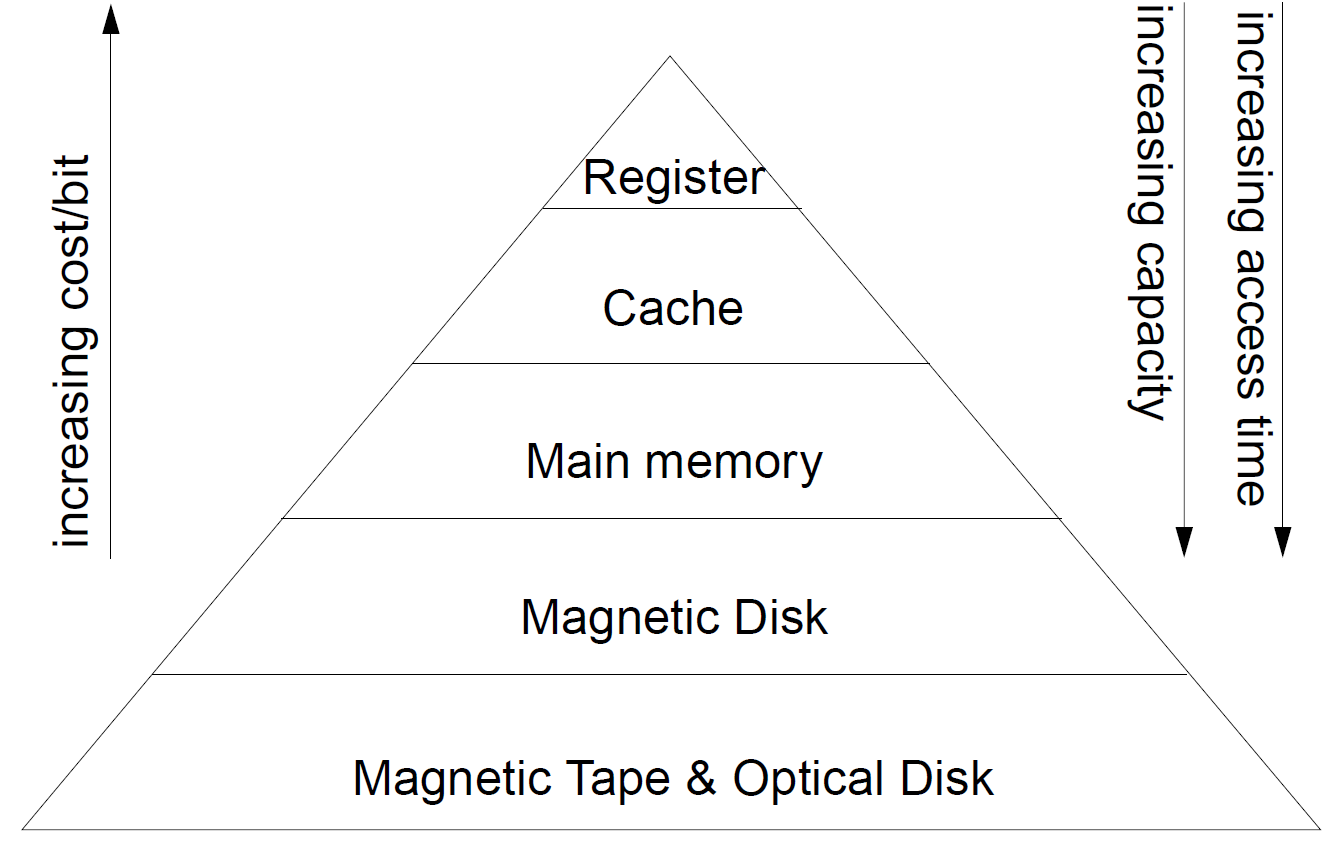
\includegraphics[width=0.7\textwidth]{mem_sys/gerarchia}
	\caption{Sistema gerarchico della memoria}
	\label{fig:gerarchia}
\end{figure}

La composizione della gerarchia è la seguente:
\begin{itemize}
\item Register file: qualche byte, tempi di accesso di qualche nanosecondo.
\item Cache on-chip (L1): qualche KB, tempi di accesso di qualche nanosecondo.
\item Cache off-chip (L2): qualche MB, tempi di accesso di decine di nanosecondi.
\item Memoria principale: qualche GB, tempi di accesso di centinaia di nanosecondi.
\item SSD o HDD: da centinaia di GB a qualche TB, tempi di accesso di decine di millisecondi.
\end{itemize}

\section{Cache}
La cache contiene copie di istruzioni e di dati presenti nelle celle della memoria principale. Il trasferimento di questo copie deve essere trasparente al processore, che non è a conoscenza dal suo punto di vista dell'esistenza della cache. Deve quindi esistere un meccanismo di predizione delle richieste del processore, per fare in modo che quando esso effettua una lettura, l'oggetto richiesto sia già disponibile immediatamente nella cache. Tutto ciò è possibile grazie all'analisi statistica degli accessi alla memoria principale, i cui risultati sono i seguenti:
\begin{itemize}
\item \textbf{Principio di località spaziale}: quando il processore accede ad una locazione di memoria è probabile che vi acceda nuovamente (come accade in un loop) o che acceda a celle adiacenti.
\item \textbf{Principio di località temporale}: quando il processore accede ad una locazione di memoria è probabile che vi acceda nuovamente nel breve termine per un numero di volte e poi non più per un lungo periodo.
\end{itemize}
Ciò significa che gli accessi non sono distribuiti uniformemente, ma in forma di cluster localizzati.

Questi principi suggeriscono di salvare nella cache i dati utilizzati più di frequente, in modo da aumentare la probabilità che essi siano prontamente disponibili su richiesta del processore. In particolare, in seguito ad un accesso si possono verificare due condizioni:
\begin{itemize}
\item \textbf{Hit}: l'oggetto richiesto è presente in cache e viene quindi trasferito immediatamente al processore, senza penalità nelle prestazioni.
\item \textbf{Miss}: l'oggetto richiesto non è presente in cache, quindi il processore deve essere fermato mentre esso viene recuperato dalla memoria principale e salvato in cache.
\end{itemize}
Il rapporto tra il numero di hit (miss) e il numero totale di accessi è detto \textbf{hit ratio} (miss ratio). In cache che funzionano bene il hit ratio è superiore al 95\%. Tuttavia è bene ricordare che si parla sempre di un'analisi statistica: possono esistere applicazioni in cui la cache non è efficace, quindi non si può assumere che essa funzionerà necessariamente bene, ma bisogna confrontare la statistica di accessi della propria applicazione con il comportamento della cache stessa. Anzi, possono addirittura essere scritte applicazioni che portano ad un 100\% di miss ratio, nel qual caso o si accetta la loro lentezza oppure è necessario riprogettarle.

Dal punto di vista dell'implementazione, si può mettere una sola cache condivisa tra dati e istruzioni, oppure, come nel caso delle architetture Harvard, si possono progettare due cache separate per istruzioni e dati. Questa seconda soluzione potrebbe essere la più efficace dal momento che le statistiche di accesso ad istruzioni e dati sono profondamente diverse (perché, ad esempio, le istruzioni vengono solo lette), ma porta alla necessità di prevedere algoritmi di salvataggio in cache diversi. Molti microcontrollori dotati di cache controller, nell'ottica di consentire al progettista il \emph{tayloring} del sistema in base alle proprie esigenze, permettono di scegliere se usare la cache solo per le istruzioni, solo per i dati o per entrambi.

\subsection{Algoritmi di mapping}
Quando il processore accede ad una locazione di memoria, serve un metodo veloce per stabilire se il dato richiesto sia presente all'interno della cache e, in caso affermativo, dove risieda. Queste tecniche vengono chiamate algoritmi di mapping e devono venire necessariamente eseguite in hardware, dal momento che devono essere trasparenti al processore.

Per il principio di località spaziale, in tutti questi algoritmi non si tratta come unità elementare la singola word, ma un insieme di word chiamati \textbf{blocchi} per la memoria principale e \textbf{linee} per la cache. Questo è in perfetto accordo con la possibilità, prevista ad esempio nelle SDRAM DDR, di effettuare accessi a burst che permettono di trasferire un blocco all'incirca nello stesso tempo di trasferimento di una singola word. Per questo motivo, inoltre, la lunghezza di tale burst è spesso impostabile dall'utente.

Per la trattazione seguente, è utile definire le seguenti quantità:
\begin{itemize}
\item $B$: il  numero di blocchi nella memoria principale.
\item $W$: il numero di word nella memoria principale, ovvero l'intero spazio di indirizzamento a disposizione del processore.
\item $L$: il numero di linee nella cache, ovvero la massima quantità di blocchi che possono essere memorizzati nella cache.
\item $b = \log_2(B)$
\item $w = \log_2(W)$
\item $l = \log_2(L)$
\end{itemize}

\subsubsection{Direct mapping}
L'algoritmo più semplice prevede che ogni blocco della memoria principale possa essere memorizzato in una sola linea di cache in modo predeterminato. In particolare, il blocco 0 viene mappato nella linea 0, il blocco 1 nella linea 1 e così via fino al blocco $L-1$. Una volta terminata la capacità della cache, si mappano i blocchi successivi nuovamente dalla prima linea: il blocco $L$ viene mappato anch'esso nella linea 0, il blocco $L+1$ nella linea 1 eccetera. 

In pratica, per decidere la destinazione di ogni blocco viene effettuata un'operazione di modulo, ovvero vengono presi gli $l$ bit meno significativi dell'indirizzo del blocco per generare l'indirizzo della linea di cache corrispondente. I restanti $b-l$ bit, ovvero la parte alta di tale indirizzo, vengono salvati insieme alla linea in un campo chiamato \textbf{tag}, che viene confrontato al momento dell'accesso con la parte alta dell'indirizzo proveniente dal processore per verificare se, in quella data linea, è memorizzato proprio quel blocco (figura \ref{fig:direct_mapping}).

\begin{figure}[hbtp]
	\centering
	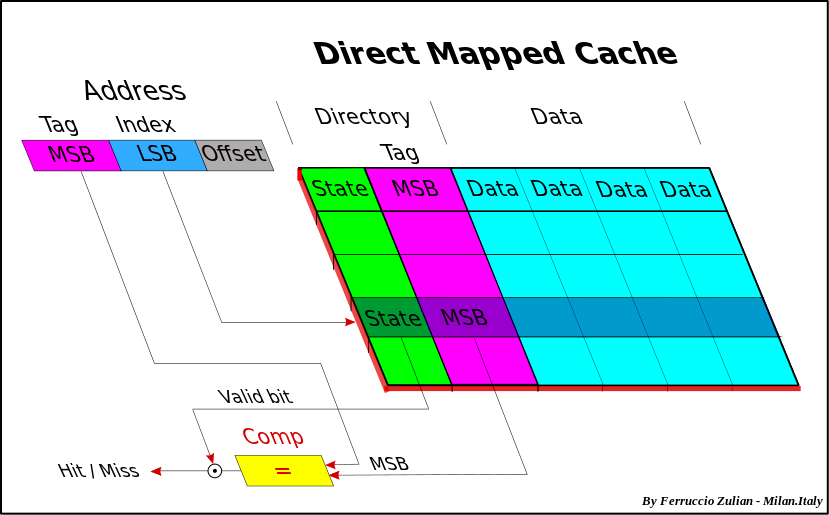
\includegraphics[width=0.7\textwidth]{mem_sys/direct_mapping}
	\caption{Direct mapping}
	\label{fig:direct_mapping}
\end{figure}

In realtà, però, il processore non è a conoscenza dei blocchi come unità fondamentale, ma esso effettua accessi soltanto a word, dando in uscita quindi indirizzi su $w$ bit. Di questi, entrano nella cache soltanto i $b$ bit più significativi che costituiscono appunto l'indirizzo del blocco. La cache fornisce in uscita sempre tutta la linea memorizzata ed i restanti $w-b$ bit vengono successivamente utilizzati per stabilire quale word all'interno di tale linea inviare al processore, agendo così come un \textbf{offset} nella linea.

Il tempo di accesso per tirare fuori la linea è quello della SRAM con cui la cache direct mapped è implementata, quindi non c'è penalità nelle prestazioni fintanto che tale tempo di accesso è confrontabile con la frequenza del processore. Il contenuto della linea è fornito in uscita a prescindere ad ogni tentativo di accesso: se il dato è presente, quindi, non è richiesta nessuna ulteriore operazione in quanto esso è già stato dato al processore; se invece non è valido, bisogna fermare il processore e trasferire il dato dalla memoria principale.

Se il vantaggio principale del direct mapping è la sua semplice implementazione hardware, lo svantaggio più significativo consiste nel fatto che il hit ratio può subire un tracollo se si accede spesso a blocchi che distano esattamente $L$ tra loro, in quanto ognuno di essi rimpiazza il precedente sempre nella stessa linea, generando costantemente un miss. Questa situazione non è così improbabile: spesso, quando si lavora con strutture dati, i compilatori eseguono come ottimizzazione un \emph{padding} in modo da allungare la struttura fino alla potenza di 2 successiva in modo da poter calcolare l'indirizzo di ogni campo di tale struttura eseguendo solo uno shift invece di una moltiplicazione, ma se così facendo la dimensione della struttura diventa un multiplo della lunghezza della cache quella che doveva essere un'ottimizzazione rende l'applicazione quasi inutilizzabile. Per tener traccia di simili eventualità, in alcuni microcontrollori ci sono dei \textbf{performance counter} in cui si possono leggere in tempo reale hit e miss ratio.

\subsubsection{Set associative mapping}
Per ovviare a questi problemi, al posto di mappare ogni blocco in in una linea sola, si raggruppa le linee in insiemi chiamati \textbf{set}, formati tipicamente da 2, 4 o 8 linee. In questo modo, un blocco può essere salvato non solo in una linea, ma in un intero set (figura \ref{fig:set_associative}).

\begin{figure}[hbtp]
	\centering
	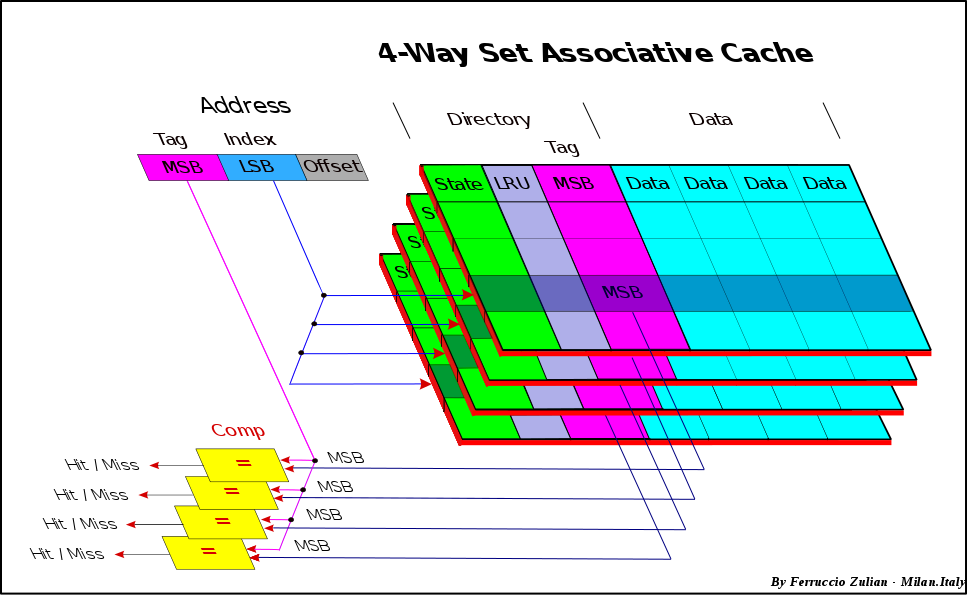
\includegraphics[width=0.7\textwidth]{mem_sys/set_associative}
	\caption{4-way set associative mapping}
	\label{fig:set_associative}
\end{figure}

Per poter memorizzare, nel caso di un algoritmo 2-way set associative, due linee insieme all'interno della SRAM, essa deve avere un array di memoria con il doppio delle colonne e la metà delle righe rispetto al caso direct mapping. Detto quindi $S$ il numero di set e $s=\log_2(S)$, si ha che l'indirizzo della cache sarà in generale dato da $l-s$ bit. Per ogni linea, come prima, viene salvato anche un tag che in questo caso però sarà formato da $s$ bit in più, per poter distinguere i diversi blocchi salvati nel set.

A fronte di una minore probabilità di avere hit ratio bassi, quindi, lo svantaggio dell'approccio set associative è di avere un hardware leggermente più complesso con più comparatori e più celle di memoria necessarie.

\subsubsection{Fully associative mapping}
Estremizzando il caso precedente, si può decidere che ogni blocco possa essere memorizzato su qualsiasi linea, di fatto creando una cache con un solo set formato da tutte le linee (figura \ref{fig:fully_associative}). Sono raramente utilizzate in quanto presentano pochi benefici rispetto al caso set associative, a fronte di un enorme aumento nel numero di comparatori. Per questo motivo, non possono essere implementate con una SRAM, ma necessitano di una \textbf{CAM} (Content Addressable Memory), in cui un comparatore è integrato in ogni cella di memoria.

\begin{figure}[hbtp]
	\centering
	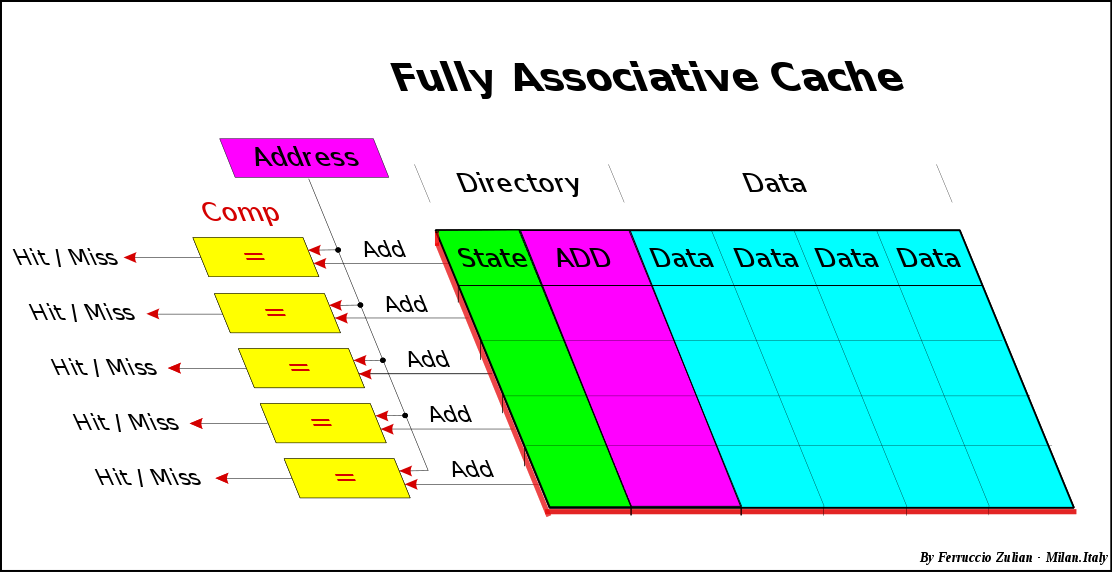
\includegraphics[width=0.7\textwidth]{mem_sys/fully_associative}
	\caption{Fully associative mapping}
	\label{fig:fully_associative}
\end{figure}

\subsection{Algoritmi di replacement}
Nelle cache set associative e fully associative, in caso di miss bisogna poter decidere quale linea nel set rimpiazzare. A tal proposito esistono numerosi algoritmi utilizzati.
\begin{itemize}
\item \textbf{Random}: si sceglie quale linea rimpiazzare generando un numero casuale in modo non polarizzato, il che non è banale da fare in hardware.
\item \textbf{LRU} (Least Recently Used): si rimpiazza la linea che da più tempo non viene utilizzata. Questa informazione va salvata in qualche modo in un \emph{timestamp}. Spesso dall'analisi si scopre che è il metodo più efficente.
\item \textbf{FIFO} (First-In-First-Out): viene rimpiazzata la linea più vecchia nel set.
\item \textbf{LFU} (Least Frequentrly Used): viene rimpiazzata la linea che è stata letta meno volte. Questo metodo necessita di un contatore per tener traccia degli accessi effettuati ad ogni linea nel set.
\end{itemize} 

\subsection{Scrittura}
In scrittura, il processore pone sul bus il dato che deve essere salvato in memoria principale, senza sapere che in mezzo è frapposta la cache. Quindi esistono diversi metodi per trasferire la scrittura destinata alla memoria principale dalla cache ad essa.
\begin{itemize}
\item \textbf{Write through}: il dato viene scritto contemporaneamente sia in cache che in memoria, fermando il processore.
\item \textbf{Buffered write through}: il dato viene scritto in cache e in un buffer temporaneo, poi con calma trasferito nella memoria principale senza interrompere il processore. Nel caso di scritture consecutive non funziona perché dalla seconda il buffer è pieno e quindi il processore va fermato.
\item \textbf{Copy-back}: il dato viene scritto solo nella cache e trasferito alla memoria principale soltanto nel momento in cui tale linea verrà rimpiazzata in seguito ad un miss. Non si ha penalità in quanto il processore dovrà già fermarsi a causa del miss. Lo svantaggio sta nel fatto che così non viene mantenuta la coerenza dei dati in memoria principale, utile nel caso essa sia condivisa tra più core. La soluzione sta nell'introdurre la possibilità di marcare a livello software alcune locazioni di memoria come \textbf{non-cachable}, in modo che le variabili memorizzate lì vengano sempre trasferite direttamente tra processore e memoria principale.
\end{itemize}

\section{Memoria virtuale}
Mentre la cache serve a non fermare il processore negli accessi alla lenta memoria principale, la memoria virtuale indica invece un insieme di tecniche messe in atto dal sistema operativo al fine di far credere al processore che ci sia una quantità di memoria principale pari all'intero spazio di indirizzamento. Nella realtà questa condizione è molto rara, infatti tipicamente la memoria principale presente nel sistema non riempie tutto lo spazio di indirizzamento disponibile, specialmente nei sistemi embedded.

Anche questo sistema è del tutto trasparente al processore: esso fornisce in uscita un indirizzo compreso nel suo spazio di indirizzamento che quindi non ha necessariamente una corrispondenza con un indirizzo fisico e, per questo motivo, viene chiamato \textbf{indirizzo virtuale}. È compito di un'unità detta \textbf{Memory Management Unit (MMU)} tradurre in una locazione fisica tale indirizzo virtuale e fornire il dato richiesto al processore.

I dati che non stanno nella memoria principale vengono salvati sulla memoria secondaria (HDD o SSD), quindi la MMU ha anche il compito di reperire i dati dal disco e caricarli in memoria principale qualora non siano già presenti. Se invece l'indirizzo virtuale ha già una corrispondenza con un indirizzo fisico in memoria principale, il dato viene trasferito automaticamente al processore senza penalità nelle prestazioni, come già accadeva nella cache. Uno schema riassuntivo è presentato in figura \ref{fig:virtual_memory}.

\begin{figure}[hbtp]
	\centering
	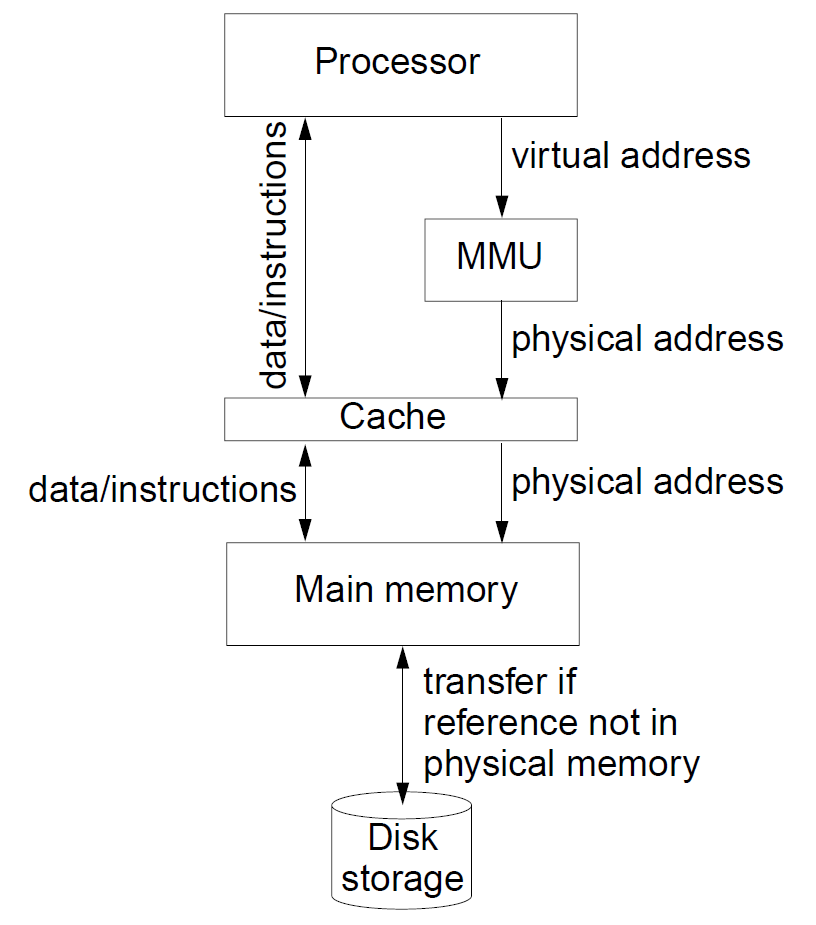
\includegraphics[width=0.5\textwidth]{mem_sys/virtual_memory}
	\caption{Schema di principio della memoria virtuale. La cache non è rilevante e potrebbe anche non essere presente.}
	\label{fig:virtual_memory}
\end{figure}

\subsection{Demand paging}
Per mappare la memoria secondaria nella memoria principale, viene usata una tecnica del tutto simile a quella delle cache: la memoria principale viene divisa in unità elementari dette \textbf{frame} e quella secondaria in \textbf{pagine}. Frame e pagine contengono lo stesso numero di word e costituiscono la minima unità che viene scambiata tra le due memorie (figura \ref{fig:frames_pages}).

\begin{figure}[hbtp]
	\centering
	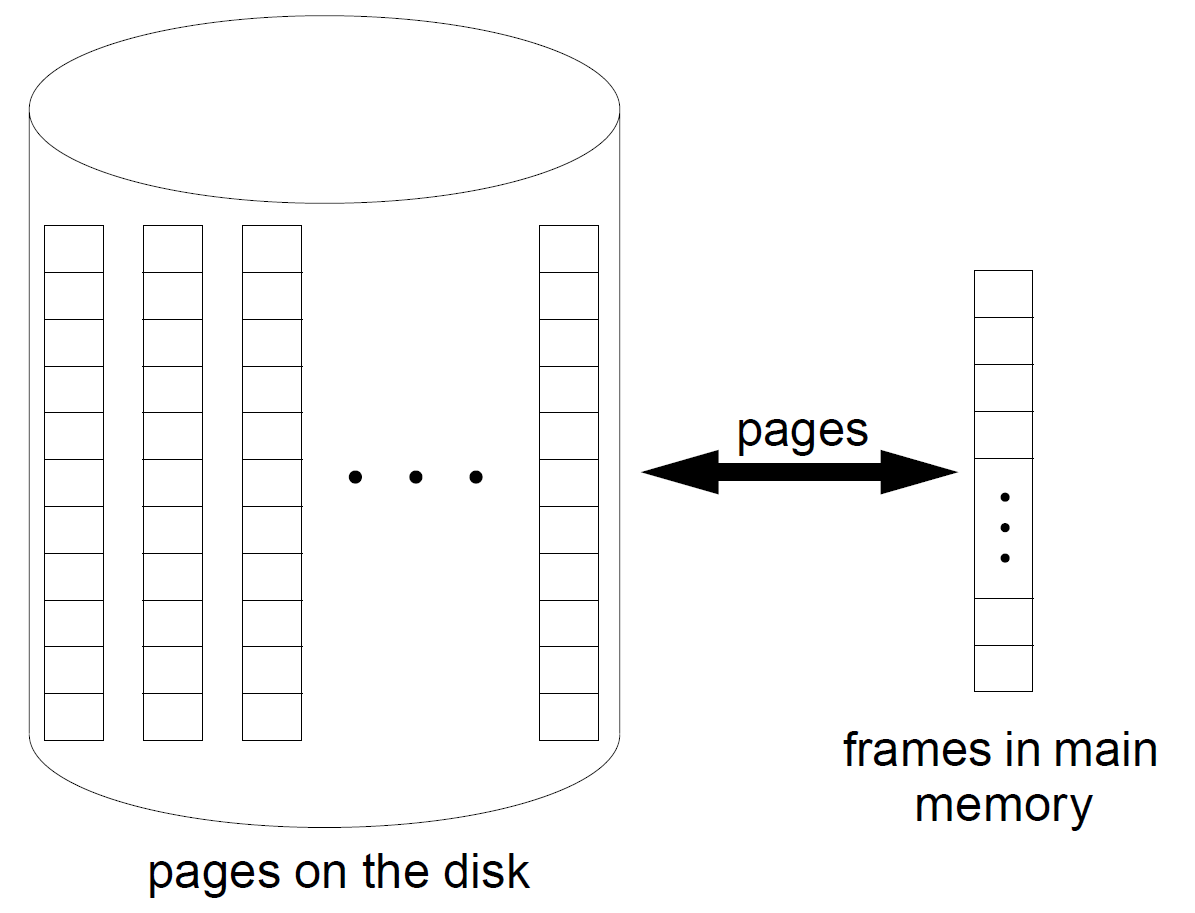
\includegraphics[width=0.5\textwidth]{mem_sys/frames_pages}
	\caption{Corrispondenza tra frame e pagine}
	\label{fig:frames_pages}
\end{figure}

In realtà, quasi mai il disco contiene tutte le pagine necessarie a riempire lo spazio di indirizzamento: il numero di pagine salvate è ristretto alla porzione di memoria virtuale effettivamente utilizzata in un dato momento. Le informazioni riguardanti queste pagine presenti su disco sono salvate in una struttura, chiamata \textbf{page table}, che contiene alcuni bit di controllo sullo stato della pagina e l'indirizzo fisico del frame di memoria corrispondente, se tale pagina è presente anche in memoria principale. Quando si alloca una pagina sul disco, quindi, è necessario aggiungere una riga relativa nella page table. Si noti che, dal momento che tale page table può essere molto grande e che a priori non è nota la statistica degli accessi alle pagine, non vengono utilizzati algoritmi di mapping, ma ogni pagina può essere assegnata a qualunque frame.

Il principale problema di questo sistema sta nel fatto che, date le sue dimensioni elevate, la page table viene salvata anch'essa su disco e quindi l'accesso a tale tabella diventa molto lento. La soluzione consiste nell'utilizzare tecniche di memoria virtuale per la page table stessa: tutte le volte che il processore accede ad una pagina, e quindi questa viene mappata su un frame, si copia anche la riga corrispondente della page table appena usata nella memoria principale. Tuttavia, ciò non basta ancora perché anche la memoria principale non è sufficientemente veloce per il processore. Quindi si utilizza una speciale memoria piccola e veloce, presente dentro la MMU, chiamata \textbf{Translation Lookaside Buffer (TLB)} che è a tutti gli effetti una cache per la page table tra la memoria principale e il processore.

In definitiva, la page table stessa è distribuita in tutta la gerarchia di memoria: la tabella intera è presente nella memoria secondaria, le righe più utilizzate in quella principale e solamente le più recenti nel TLB.

\subsection{Traduzione degli indirizzi}
La decodifica degli indirizzi da parte della MMU risulta quindi banale: si prende l'indirizzo virtuale composto da una parte alta che indica il numero di pagina ed una parte bassa che indica l'offset di una word nella pagina, si cerca tale numero di pagina nella page table e, se presente in memoria, si sostituisce nella parte alta dell'indirizzo con il numero di frame corrispondente.

Se invece la pagina richiesta non è presente nella memoria principale, si ha un cosiddetto \textbf{page fault}, ovvero il corrispondente del miss nella cache. In questo caso entra in gioco il sistema operativo che va a caricare la pagina richiesta in memoria principale e modifica la riga corrispondente nella page table. Se non ci sono frame disponibili, si impiegano algoritmi di replacement del tutto simili a quelli usati nelle cache per decidere quale sostituire. Si noti che, dal momento che l'accesso alla memoria secondaria è piuttosto lento, tale procedura viene gestita a livello puramente software, tipicamente con un interrupt, in quanto implementarla in hardware (come invece avviene in caso di miss della cache) sarebbe del tutto un spreco.
In figura \ref{fig:vm_flow} è illustrato un diagramma del flusso delle operazioni effettuate dalla MMU.

\begin{figure}[hbtp]
	\centering
	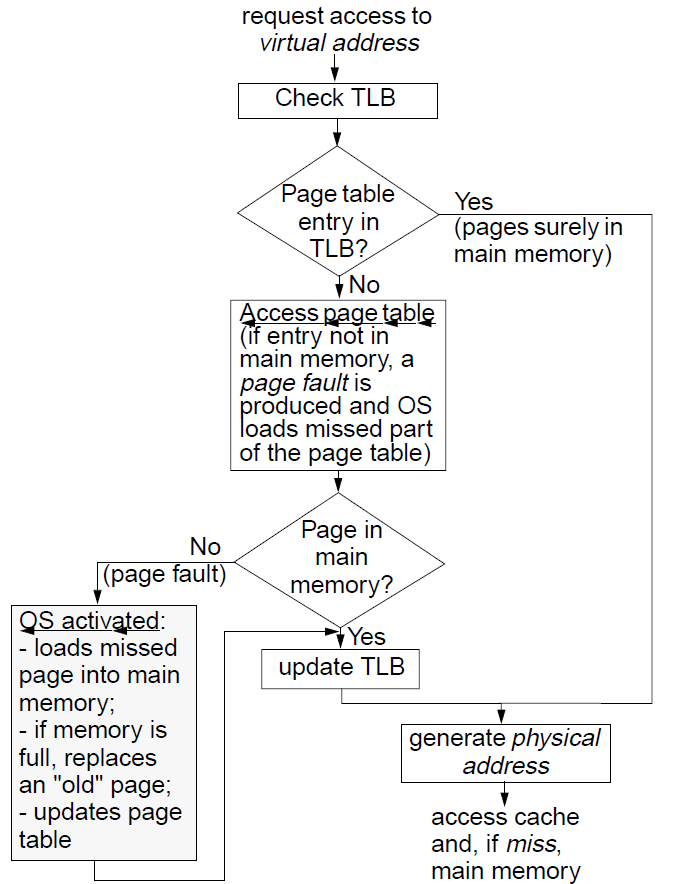
\includegraphics[width=0.6\textwidth]{mem_sys/vm_flow}
	\caption{Flow chart del sistema di memoria virtuale}
	\label{fig:vm_flow}
\end{figure}

Solitamente gli indirizzi virtuali della memoria codice vengono tenuti separati da gli indirizzi virtuali dei dati, in modo da poter garantire l'integrità con dei particolari flag relativi ai permessi di lettura, scrittura o esecuzione.

Infine, è bene sottolineare che il sistema di memoria virtuale funziona solo se non serve tutta la memoria indirizzabile non serve contemporaneamente, altrimenti il sistema diventa estremamente lento perché si trova continuamente a dover effettuare accessi alla memoria secondaria per caricare le pagine richieste. Tale situazione è nota come \textbf{crashing}.

\section{Direct Memory Access (DMA)}
Un tipico sistema embedded possiede un bus a cui sono collegati il microcontrollore, una memoria RAM, una ROM e delle periferiche. Proprio la parte di I/O può essere dominante dal punto di vista delle prestazioni, rispetto alla potenza di calcolo, come succede ad esempio in uno switch di rete. Ciò significa che le prestazioni dipendono pesantemente dalla capacità di trasferire i dati dall'I/O alla memoria. In una condizione standard, quando arriva un dato, il peripheral chip invia un interrupt al microprocessore che quindi salva lo stato corrente nello stack, carica le istruzioni della ISR, salva il dato nel proprio register file, effettua una scrittura nella RAM e infine ripristina lo stato leggendo dallo stack. Tutta questa sequenza di istruzioni rende la procedura estremamente inefficiente, in quanto l'obiettivo finale era semplicemente trasferire il dato dalla periferica alla RAM. Ciò significa quindi che, nel caso in cui l'I/O viaggi ad alta velocità, il microprocessore non riesce a tenerne il passo.


La soluzione consiste nel mettere un coprocessore hardware che si occupi esclusivamente dei trasferimenti tra I/O e memoria, ma che li esegua in modo estremamente veloce ed efficace. Questo meccanismo si chiama DMA e il componente hardware che lo gestisce viene detto \textbf{DMA Controller (DMAC)}. 

Con questo sistema, quando la periferica ha dei dati pronti non manda l'interrupt, ma manda solo una richiesta al DMAC. Il controllore quindi dà un ACK di conferma alla periferica e contemporaneamente abilita la RAM in scrittura, creando quindi un percorso diretto tra la periferica e la memoria, in modo che una word sia trasferita in un solo ciclo di bus. Il processore non rientra in questa operazione e quindi, nel frattempo, ha potuto eseguire altro codice, magari salvato in cache, senza neanche accorgersi che il bus è stato momentaneamente occupato. In questo modo le prestazioni aumentano di ordine di grandezza.

Il DMAC, tuttavia, non lavora in modo indipendente: il processore deve comunicare al DMAC l'indirizzo in cui iniziare a salvare i dati che provengono dalle periferiche, chiamato \textbf{base address}, e il numero di word che si aspetta di leggere in totale. Queste informazioni vengono memorizzate in un registro interno al DAMC ed un contatore quindi viene incrementato ad ogni trasferimento in modo da salvare i dati in celle di memoria contigue, fino al raggiungimento del numero di dati previsto. Quando la procedura è quasi completa, il DMAC invia un interrupt al processore che gli comunica un nuovo base address. Il numero di interrupt è comunque particolarmente ridotto rispetto al caso senza DMA.

\begin{tcolorbox}[breakable,enhanced]
\textbf{Asymmetric multiprocessing}\\
In un sistema capace di effettuare asymmetric multiprocessing, sono presenti diversi core, o diversi coprocessori, ognuno dedicato ad una specifica funzione. Il DMA può essere visto proprio come un esempio di tale paradigma, in quanto permette al microprocessore di effettuare altre operazioni mentre il DMAC si occupa della gestione delle periferiche. Ad esempio, nel caso della ricezione di pacchetti di rete, il processore può già elaborare l'intestazione del pacchetto e stabilire la sua destinazione prima ancora che il DMAC ne abbia salvato tutto il contenuto. Addirittura, in alcuni microcontrollori specializzati per le telecomunicazioni, il DMAC è in realtà un piccolo processore RISC con una ISA estremamente ridotta (8 istruzioni) che permette però di eseguire delle pre-elaborazioni sui dati ricevuti che sarebbero decisamente onerose per il processore, come la trasposizione di una matrice.

Un altro esempio di asymmetric multiprocessing è dato da alcuni sistemi embedded in cui è presente un core ad alta potenza di calcolo ma ad alta latenza su cui c'è Linux come sistema operativo ed un secondo core più piccolo, ma più reattivo su cui può girare un RTOS come MQX.
\end{tcolorbox}



\chapter{Interfacce seriali}
Molto spesso progettando sistemi digitali ci si imbatte nel problema dell'interfacciamento con periferiche esterne. A tal fine vengono impiegate nella maggior parte dei casi interfacce con protocolli standard commerciali e non definiti \emph{ad hoc}. In particolare, le più diffuse sono le interfacce seriali, dal momento che, per il ridotto numero di fili che richiedono, rappresentano una scelta efficace in termini di costo. 

Di bus seriali ne esistono un numero elevatissimo, sia sincroni che asincroni: da quelli general purpose come RS232, SPI, \iic\ o USB, a quelli application specific come CAN (automotive), $\text{I}^2\text{S}$, S/PDIF o AES3 (audio professionale). In questo contesto verranno analizzati in dettaglio soltanto \iic\ e SPI, che sono tra i più comuni nell'interfacciamento tra periferiche a livello di scheda. Non saranno invece trattati RS232 ed USB perché più adatti a collegare dispositivi fisicamente diversi (come ad esempio un PC ed una stampante). Inoltre USB, per essere il più \emph{universal} possibile, sposta gran parte del protocollo sul software, che quindi va scritto singolarmente per ogni dispositivo. Risulta perciò uno standard più complesso e pesante, sprecato nel caso in cui si conoscano in anticipo le caratteristiche delle periferiche da collegare.

\section{\iic\ (Inter Integrated Circuit)}
Il protocollo \iic\ è stato pensato per essere il più semplice ed a basso costo possibile, pur permettendo di collegare tra loro un master e più slave. A tal fine, utilizza un bus di tipo open collector, in cui quindi le periferiche collegate possono soltanto comandare uno 0 logico, mentre l'1 è dato dalla resistenza di pull-up collegata all'alimentazione (figura \ref{fig:busiic}). 

\begin{figure}[hbtp]
	\centering
	% XCircuit output "iic.tex" for LaTeX input from iic.eps
\def\putbox#1#2#3#4{\makebox[0in][l]{\makebox[#1][l]{}\raisebox{\baselineskip}[0in][0in]{\raisebox{#2}[0in][0in]{\scalebox{#3}{#4}}}}}
\def\rightbox#1{\makebox[0in][r]{#1}}
\def\centbox#1{\makebox[0in]{#1}}
\def\topbox#1{\raisebox{-0.60\baselineskip}[0in][0in]{#1}}
\def\midbox#1{\raisebox{-0.20\baselineskip}[0in][0in]{#1}}
\begin{center}
   \scalebox{1}{
   \normalsize
   \parbox{2.02604in}{
   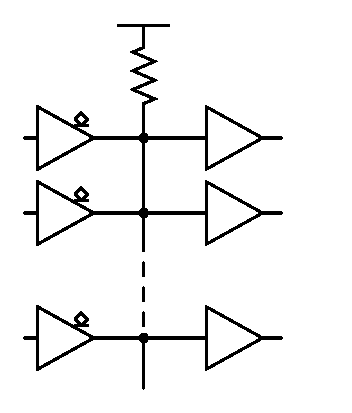
\includegraphics[scale=1]{seriali/iic.eps}\\
   % translate x=568 y=208 scale 0.38
   \putbox{1.01in}{2.14in}{1.20}{$R_{PU}$}%
   } % close 'parbox'
   } % close 'scalebox'
   \vspace{-\baselineskip} % this is not necessary, but looks better
\end{center}

	\caption{Bus \iic\ open collector}
	\label{fig:busiic}
\end{figure}

Con questa configurazione, quando un dispositivo forza uno 0 sul bus, esso risponde in un tempo nell'ordine delle decine di \si{\nano\second}, tuttavia, quando invece il dispositivo si toglie dal bus, la velocità di risposta è quella di un sistema del primo ordine con costante di tempo data da $\tau = R_{PU}C$. Da qui nasce un vincolo sulla massima capacità ammessa sul bus, pari a circa \SI{200}{\micro\farad}, per evitare che il sistema diventi eccessivamente lento.

La trasmissione avviene mediante due sole linee:
\begin{itemize}
	\item \textbf{SCL} (Serial Clock Line): pilotata sempre e solo da master, non è propriamente un segnale di clock, ma uno strobe, dal momento che può anche rimanere fissa a 1 per un dato periodo di tempo. Per tale motivo il protocollo \iic\ non è propriamente sincrono, anche se spesso si può definire così ugualmente.
	\item \textbf{SDA} (Serial Data Line): può essere pilotata sia da master che da slave, a seconda di chi sta inviando dati, ovvero è sempre pilotata dal \emph{trasmettitore}.
\end{itemize}
Dal momento che la linea di dato è unica, è chiaro che \iic\ è un bus seriale \emph{half-duplex}. Un tipico schema di connessione \iic\ è mostrato in figura \ref{fig:iic_example}.
\begin{figure}[H]
	\centering
	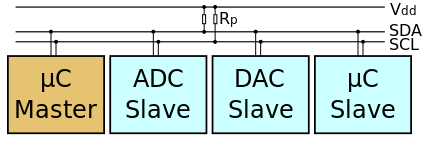
\includegraphics[width=0.5\linewidth]{seriali/iic_example.png}
	\caption{Schema \iic\ con un microcontrollore come master e tre slave}
	\label{fig:iic_example}
\end{figure}
Le due resistenze di pull-up non sono quasi mai integrate nei microcontrollori che dispongono di un'interfaccia \iic\ e quindi vanno sempre inserite come componenti discreti esterni. Tipicamente i loro valori sono nell'ordine del \si{\kilo\ohm} e ciò porta come conseguenza il fatto che, mentre lo 0 logico è particolarmente robusto data la basa resistenza dei MOS dei driver, l'1 logico è invece più sensibile ai disturbi poiché la $R_{PU}$ al contrario non è molto piccola. Ciò porta ad una limitazione sulla distanza massima possibile per i collegamenti.

\subsection{Protocollo di trasmissione}
Il protocollo \iic\ prevede che la trasmissione avvenga a 9 bit per volta: 8 bit di payload e 1 bit di acknowledgement ($\overline{ACK}$). La sequenza di passi per la trasmissione è la seguente:
\begin{enumerate}
	\item Si parte da una situazione di \textbf{idle}, in cui entrambe le linee sono a 1 e nessuno parla.
	\item Il master quindi impone la \textbf{start condition}, ovvero la transizione della linea SDA da 1 a 0, mentre SCL rimane a 1 (figura \ref{fig:iic_start}).
	\begin{figure}[H]
		\centering
		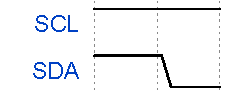
\includegraphics[width=0.3\linewidth]{seriali/start_condition}
		\caption{Start condition}
		\label{fig:iic_start}
	\end{figure}
	\item La trasmissione vera è propria può ora iniziare: il primo byte inviato contiene un indirizzo di 7 bit, che identifica il dispositivo con quale il trasmettitore vuole comunicare, ed un bit $R/\overline{W}$ per decidere se se il trasmettitore vuole leggere dati dal ricevitore o scriverli in esso. Condizione fondamentale è che la linea SDA può avere transizioni soltanto quando SCL è a 0 (figura \ref{fig:iic_transition}). Inoltre, chi riceve può così decidere di campionare su uno dei due fronti del clock, anche se spesso di sceglie il fronte di discesa per ottimizzare il tempo di setup.
	\begin{figure}[H]
		\begin{subfigure}{.5\textwidth}
			\centering
			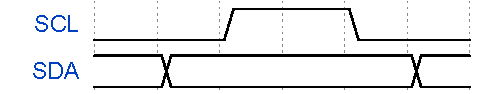
\includegraphics[width=\linewidth]{seriali/iic_correct}
			\caption{Transizione corretta}
		\end{subfigure}
		\begin{subfigure}{.5\textwidth}
			\centering
			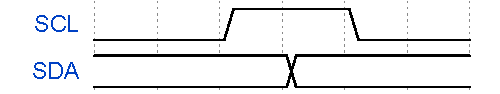
\includegraphics[width=\linewidth]{seriali/iic_error}
			\caption{Transizione errata}
		\end{subfigure}
	\caption{Condizione per una corretta trasmissione}
	\label{fig:iic_transition}
	\end{figure}
	\item La trasmissione prosegue finché il master non impone la \textbf{stop condition}, ovvero la transizione da 0 a 1 di SDA, mentre SCL rimane a 1 (figura \ref{fig:iic_stop}).
	\begin{figure}[H]
		\centering
		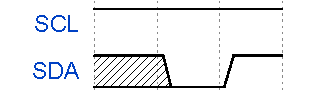
\includegraphics[width=0.3\linewidth]{seriali/stop_condition}
		\caption{Stop condition}
		\label{fig:iic_stop}
	\end{figure}
\end{enumerate}
Il bit di acknowledgement serve al ricevitore per comunicare una errata ricezione di un dato, ma può anche essere utilizzato dal master per capire quali slave sono collegati al bus, tramite un'\textbf{enumerazione}: il master inizia una trasmissione con ogni indirizzo tra 0 e 128 e rileva chi risponde dando un ack. L'indirizzo di uno slave è fissato dal costruttore della periferica, quindi bisogna accertarsi di collegare sul bus dispositivi con indirizzi tutti diversi tra loro per evitare conflitti. Alcuni costruttori, raramente, mettono a disposizione un pin per cambiare leggermente l'indirizzo, garantendo più flessibilità.

\begin{datasheet}{Atmel AT24C01x \iic-Compatible (2-wire) Serial EEPROM}{ds:atmel_iic}
Le dimensioni della memoria sono ridotte, solo \SI{128}{\byte}, perché spesso è inutile avere memorie enormi quando si vogliono salvare solo pochi parametri specifici. Ad esempio, una memoria del genere potrebbe essere utilizzata per salvare delle impostazioni come il volume di un dispositivo, oppure una chiave di cifratura, per la quale \SI{128}{\byte} rappresentano già un alto livello di sicurezza, oppure ancora un codice IMEI di un dispositivo mobile.

La velocità va da \SI{400}{\kilo\hertz}, con tensione di alimentazione \SI{1.7}{\volt}, a \SI{1}{\mega\hertz}, con tensione di alimentazione \SI{5}{\volt}. Questi valori non sono casuali: \SI{400}{\kilo\hertz} è la minima velocità stabilita dal protocollo \iic\, mentre \SI{1.7}{\volt} e \SI{4.2}{\volt} sono rispettivamente le tensioni assunte da una batteria al litio scarica e carica. Questa memoria quindi è particolarmente adatta ad applicazioni alimentate a batteria.

L'endurance dichiarata di 1000000 cicli, così come la data retention di 100 anni, conferiscono a questa memoria un'affidabilità ordini di grandezza superiore a quella di altre memorie commerciali come le flash.

Un'altra applicazione tipica di un tale chip è all'interno di moduli DIMM di RAM, per salvare informazioni utili al memory controller, quali tensione di alimentazione, frequenza massima operativa e organizzazione fisica del modulo di memoria.

Per effettuare un'operazione di lettura, il master seleziona il dispositivo con il suo indirizzo mettendo $R/\overline{W} = 0$ e quindi scrive l'indirizzo del dato che vuole leggere dalla memoria. Successivamente, impone una  nuova start condition, senza aver dato la stop condition, e scrive nuovamente l'indirizzo dello slave questa volta mettendo $R/\overline{W} = 1$, in modo da leggere i dati che arrivano dalla memoria. Questa sequenza di operazioni è nota come \textbf{repeating start}.
\end{datasheet}

\section{SPI (Serial Peripheral Interface)}
Il protocollo SPI utilizza una trasmissione tramite tre fili:
\begin{itemize}
		\item \textbf{SCK} (Serial Clock): è il clock imposto dal master a tutti gli slave.
		\item \textbf{MISO} (Master In Slave Out): linea di dato da slave a master.
		\item \textbf{MOSI} (Master Out Slave In): linea di dato da master a slave.
\end{itemize}
Dal momento che il protocollo dispone di due linee di dato separate, la comunicazione seriale può avvenire in modalità \emph{full-duplex}. I bus dei segnali SCK e MOSI sono di tipo totem pole, mentre il MISO è tri-state per poter essere pilotato da un solo slave alla volta. Entrambi i valori logici 0 e 1 possono quindi essere forzati sul bus. La velocità massima ottenibile è nell'ordine delle decine di \si{\mega\hertz}.

L'indirizzamento dei vari slave è in questo caso fisico: ogni slave ha un segnale in ingresso detto \textbf{Slave Select} ($\overline{SS}$), che viene asserito dal master per scegliere con quale dispositivo comunicare. Un tipico schema di connessione è riportato in figura \ref{fig:spi_blocks}.
\begin{figure}[hbtp]
	\centering
	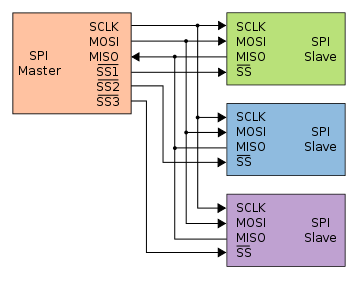
\includegraphics[width=0.5\linewidth]{seriali/spi_blocks.png}
	\caption{Protocollo SPI}
	\label{fig:spi_blocks}
\end{figure}

All'interno di master e slave, ci sono due shift register per la trasmissione e la ricezione, tipicamente da 8 bit. In sistemi più economici, può esserci invece un solo shift register. Il protocollo permette di trasmettere un numero arbitrario di bit, dal momento che la lunghezza del pacchetto non è predefinita, ma può essere adattata a quello che la periferica richiede.

\pagebreak

\begin{datasheet}{Atmel AT250x0B SPI Serial EEPROM}{}
Questa memoria è la stessa del datasheet \ref{ds:atmel_iic}. Qui il segnale $\overline{CS}$ corrisponde al $\overline{SS}$. Non essendo previsto dal protocollo il segnale $R/\overline{W}$, per leggere e scrivere bisogna prima inviare alla memoria dei comandi specifici.

In questo caso, sul fronte di salita del clock la memoria campiona il dato in ingresso e sul fronte di discesa fornisce il dato in uscita.

Non è questo il caso, ma alcuni dispositivi sfruttano la caratteristica del SPI di essere full-duplex per offrire la possibilità di fare una lettura completa di una pagina (\textbf{page read}), fornendo in uscita i dati mentre contemporaneamente in ingresso si ricevono gli indirizzi.
\end{datasheet}

\begin{datasheet}{Analog Devices AD520x Digital Potentiometer}{}
Questo potenziometro digitale permette di sostituirne uno analogico, con il vantaggio di avere dimensioni molto più compatte e di poter essere controllato da un microcontrollore.

La struttura interna consiste di una schiera di $N$ resistori in serie e $N-1$ pass transistor che permettono di selezionarli. Lo svantaggio principale è proprio rappresentato dalla resistenza di canale di tali pass transistor, che, dipendendo dalla $V_{DS}$, porta ad avere delle non linearità nel valore del potenziometro.

Applicazioni tipiche di tale dispositivo possono essere tasti per il controllo del volume, ad esempio su un telefono, o sistemi di calibrazione di strumenti di misura, come un oscilloscopio, in quanto permettono di testare in modo rapido ed automatico diversi fondo scala.
\end{datasheet}


\begin{datasheet}{Analog Devices AD7927 8-Channel, 200 kSPS, 12-Bit ADC with Sequencer}{}
La caatteristica principale di questo ADC è il fatto di possedere un \textbf{sequencer}, dispositivo che permette di configurare il convertitore per convertire in sequenza un certo numero di canali, senza dover intervenire dall'esterno.

La configurazione avviene tramite degli appositi registri di controllo scrivibili.
\end{datasheet}

\chapter{Compatibilità elettromagnetica (EMC)}
La giorno d'oggi ci sono molte apparecchiature elettroniche che, utilizzando tensioni e correnti alternate, emettono onde elettromagnetiche. Questo è dovuto al fatto che ogni tensione che varia rispetto ad un piano metallico è un'antenna trasmettente ed ogni oggetto o filo metallico non connesso a massa è un'antenna ricevente. Per questo motivo, bisogna fare in modo che più oggetti elettronici che si trovano nello stesso ambiente non si disturbino tra di loro.

Questa problematica non era molto rilevante quando i circuiti erano a valvole (molto grosse e resistenti) e il numero di dispositivi elettronici nella vita quotidiana non era grande. Oggi, invece, la miniaturizzazione dei transistor nei circuiti integrati e il costante calo delle energie in gioco nei dispositivi rende i disturbi molto più significativi a parità di intensità.

A tal proposito, la tecnologia digitale ha da un lato aumentato la resistenza a tali disturbi grazie al concetto di \textbf{margine di rumore}, ma dall'altro ha anche aumentato le sorgenti stesse di tali disturbi, quali segnali di clock e onde quadre in generale.

Al fine di introdurre delle regole riguardo la compatibilità elettromagnetica, a partire dalla fine degli anni '60, sono state applicate delle normative prima italiane (CEI) e poi europee (CENELEC) che prevedevano specifiche aggiuntive che ogni progetto elettronico doveva soddisfare, proprio nell'ambito EMC. Nel 1989, l'allora Comunità Economica Europea ha introdotto la direttiva CE con l'intenzione di armonizzare le norme, tra cui anche quelle sulla compatibilità elettromagnetica, all'epoca presenti nei diversi paesi al fine di garantire la libera commercializzazione dei prodotti all'interno del mercato europeo. La grande novità di tale direttiva consiste nel fatto che è su ogni progetto è richiesta la firma di una persona fisica che si assuma le responsabilità della conformità alle specifiche in nome del produttore.

È di fondamentale importanza tener conto di queste specifiche già in fase di progetto, per evitare che un prodotto finito debba essere riprogettato da zero in quanto non rispetta le direttive comunitarie.

\section{Metodologia di test}
I disturbi elettromagnetici possono essere sostanzialmente di due tipi:
\begin{itemize}
\item \textbf{Irradiati} nell'ambiente da antenne.
\item \textbf{Condotti} attraverso conduttori metallici, come ad esempio i disturbi di rete.
\end{itemize}
ed ognuno di questi deve essere testato in due casi:
\begin{itemize}
\item \textbf{Emissioni}, ovvero la quantità di disturbo che il dispositivo emette.
\item \textbf{Immunità}, ovvero quanto il dispositivo è resistente a tali disturbi.
\end{itemize}

Le prove riguardanti i disturbi irradiati devono essere effettuate all'interno di una \textbf{camera anecoica}, ovvero una stanza schermata dall'esterno, le cui pareti sono ricoperte da coni di materiale assorbente (plastica ricoperta di nerofumo). In realtà, per simulare uno spazio aperto, tali coni vengono posizionati su tutte le pareti tranne il pavimento, creando così una camera semianecoica (figura \ref{fig:camera_anecoica}). Dato l'elevato costo di una struttura del genere, spesso le aziende medio-piccole non ne hanno una propria ma la affittano a tempo da aziende specializzate per effettuare i test. Un'antenna in trasmissione o in ricezione ed il DUT all'interno di questa stanza permettono di misurare i disturbi irradiati emessi ed assorbiti senza guasti.

\begin{figure}[hbtp]
	\centering
	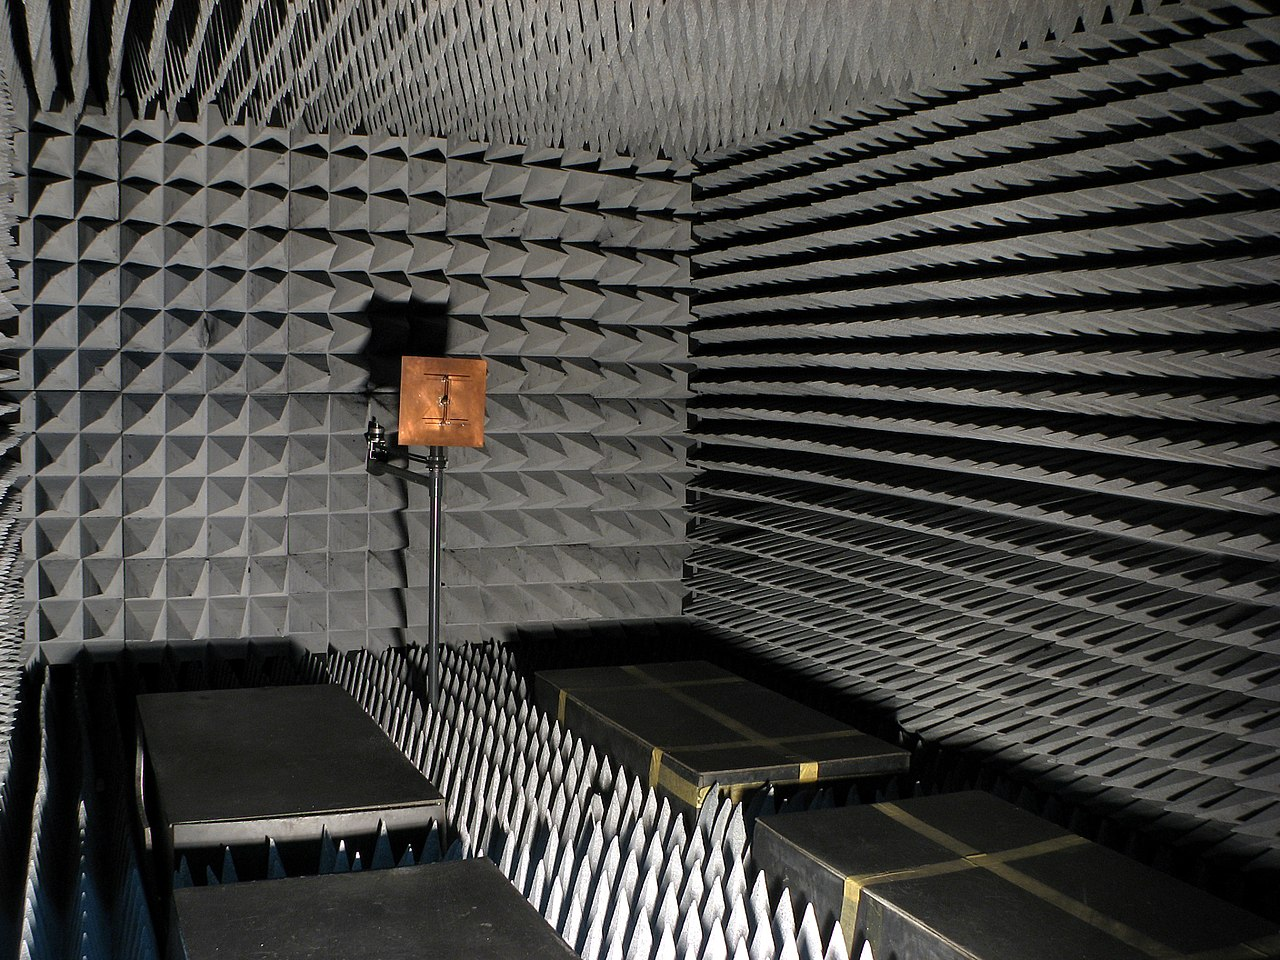
\includegraphics[width=0.6\linewidth]{emc/camera_anecoica}
	\caption{Camera anecoica}
	\label{fig:camera_anecoica}
\end{figure}

Per le prove riguardo ai disturbi condotti, invece, non serve una camera anecoica, ma basta misurare il disturbo sulla linea di alimentazione prodotto dal dispositivo o iniettato da un apposito amplificatore. Bisogna introdurre dei filtri in modo da isolare i disturbi esterni.

In generale, le metodologie utilizzate per ridurre entrambi i tipi di disturbi sono simili, data la correlazione tra loro: ad esempio, dei disturbi condotti sui cavi di alimentazione generano dei disturbi irradiati tramite gli stessi cavi.

\section{Disturbi irradiati}
Nel mondo digitale i segnali che si trattano sono teoricamente onde quadre, ma in realtà sono segnali del tutto analogici e per questo motivo in prima approssimazione verranno trattati come segnali di forma trapezoidale (figura \ref{fig:trapezio}), con una certa ampiezza, un certo periodo e un duty cycle medio calcolato sul segnale reale non periodico.

\begin{figure}[hbtp]
	\centering
	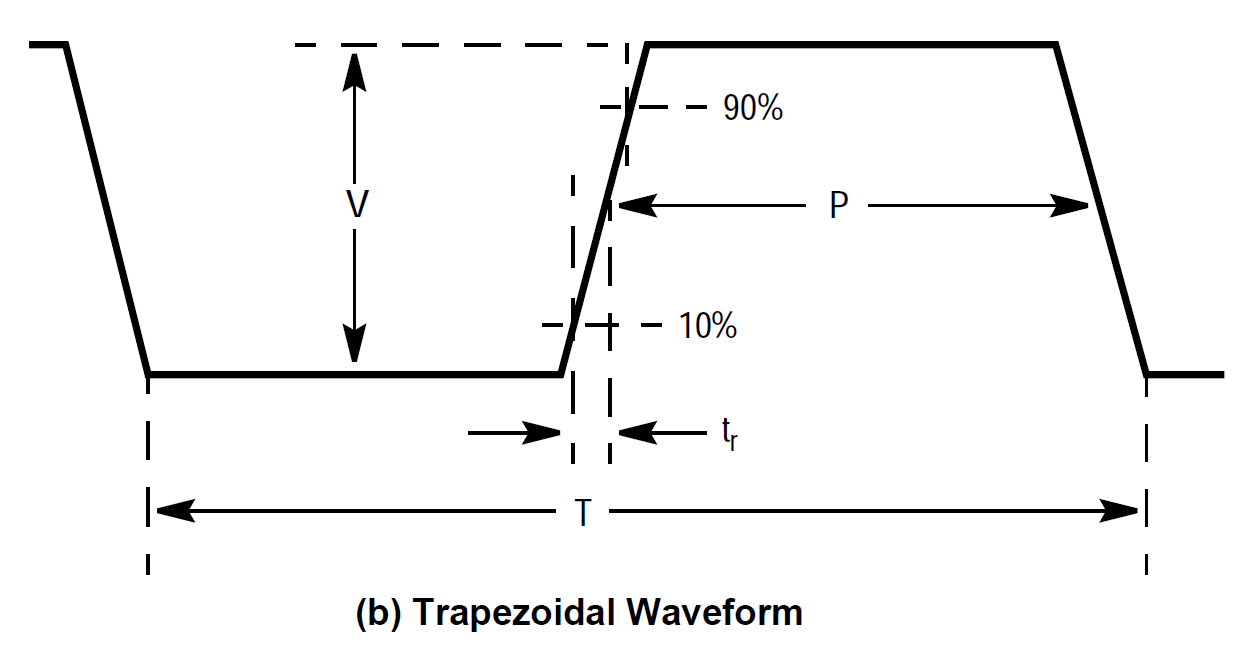
\includegraphics[width=0.6\linewidth]{emc/trapezio}
	\caption{Segnale trapezoidale}
	\label{fig:trapezio}
\end{figure}

Ne consegue che lo spettro in frequenza non è quello a righe tipico di un'onda quadra, ma si può dimostrare che rientra sempre nel grafico \emph{worst case} di figura \ref{fig:spettro_trapezio}. Esso presenta un'ampiezza costante fino alla frequenza $f_1 = 1/(\pi P)$, inversamente proporzionale al (semi)periodo del segnale, poi inizia a diminuire a \SI{-20}{dB/dec} fino ad una frequenza $f_2=1/(\pi t_r)$, inversamente proporzionale al tempo di salita del segnale, oltre la quale scende a \SI{-40}{dB/dec}.

\begin{figure}[hbtp]
	\centering
	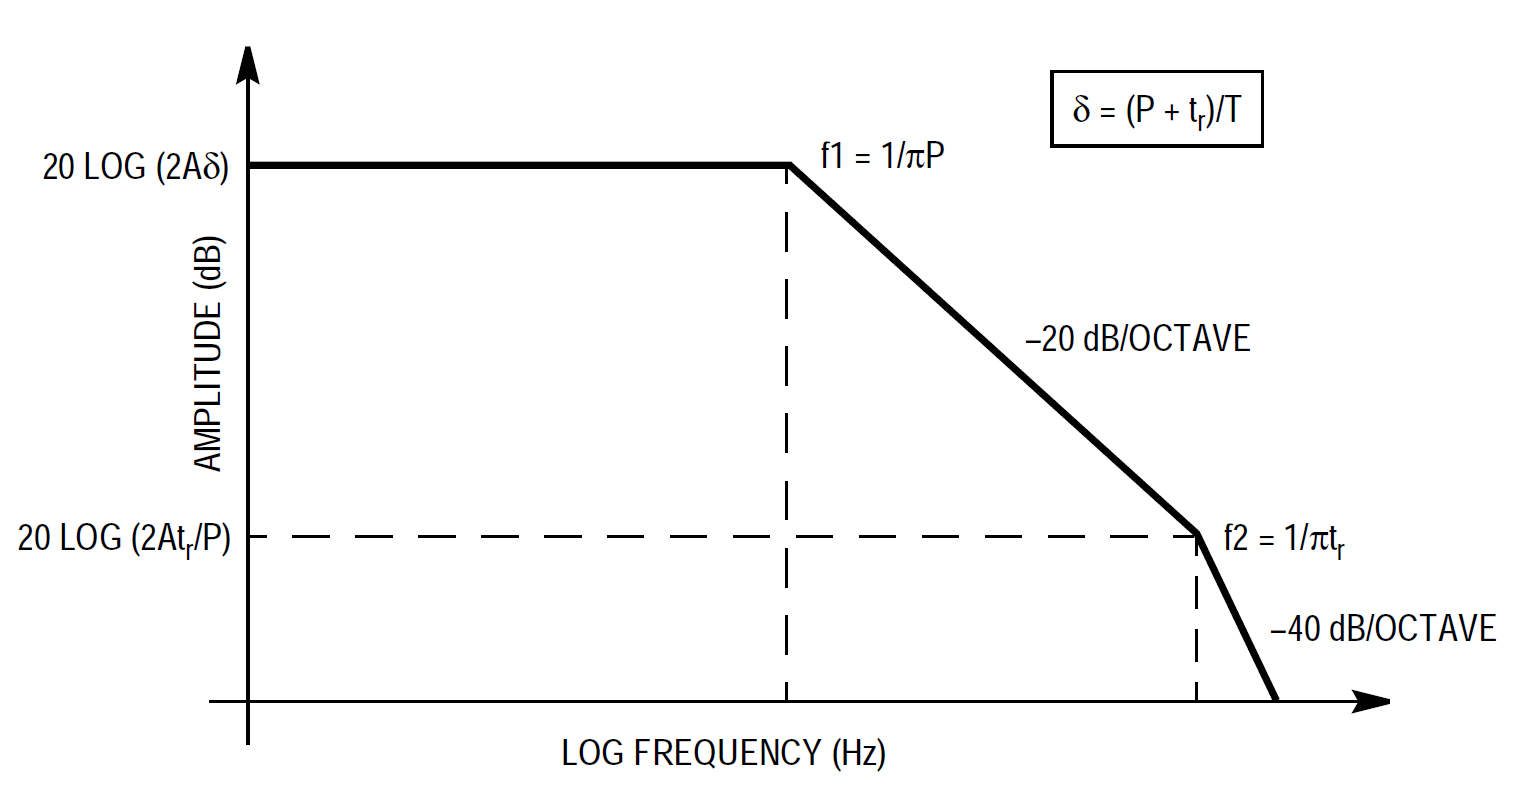
\includegraphics[width=0.6\linewidth]{emc/spettro_trapezio}
	\caption{Spettro di un segnale trapezoidale}
	\label{fig:spettro_trapezio}
\end{figure}

Quando una sorgente che emette un segnale di questo tipo è collegata ad un'antenna, si possono generare due tipologie di disturbi irradiati:
\begin{itemize}
\item Disturbi di \textbf{modo differenziale}, se l'antenna irradia un campo magnetico $H$, ovvero è formata da una spira percorsa da corrente (figura \ref{fig:loop}). È chiamato così perché alla spira viene applicata una \emph{differenza} di potenziale.
\item Disturbi di \textbf{modo comune}, se l'antenna irradia un campo elettrico $E$, ovvero è formata da un dipolo elettrico (figura \ref{fig:dipole}). È chiamato così perché il conduttore del dipolo è collegato al riferimento \emph{comune} di massa.
\end{itemize}

\begin{figure}[hbtp]
	\centering
	\begin{subfigure}{.3\textwidth}
		\centering
		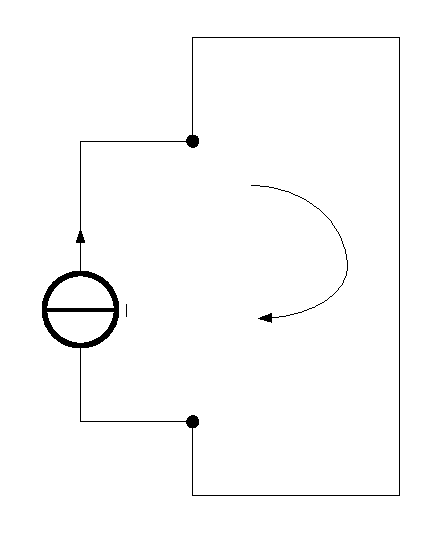
\includegraphics[width=\linewidth]{emc/loop}
		\caption{Spira}
		\label{fig:loop}
	\end{subfigure}
	\begin{subfigure}{.5\textwidth}
		\centering
		\includegraphics[width=\linewidth]{emc/dipole}
		\caption{Dipolo}
		\label{fig:dipole}
	\end{subfigure}
	\caption{Due tipi di antenne}
\end{figure}

\subsection{Disturbo di modo differenziale}
Si può dimostrare che in condizioni di campo lontano, la componente del campo elettrico irradiato per un disturbo di modo differenziale è data da:
\begin{equation}
	E = 2.6\ \frac{AI_L f^2}{R} \quad [\si{\micro\volt\per\meter}]
\end{equation}
dove:
\begin{description}
	\item $A$: area della spira
	\item $I_L$: corrente nella spira
	\item $f$: frequenza
	\item $R$: distanza dall'antenna
\end{description}

Si noti che la dipendenza da $R$ è (inversamente) lineare e non quadratica in quanto l'equazione si riferisce solamente alla componente di campo elettrico del campo elettromagnetico. Il termine più fastidioso è la dipendenza quadratica dalla frequenza, perché indica che lo spettro cresce costantemente a \SI{40}{dB/dec}. Considerando questa come funzione di trasferimento e moltiplicando per un segnale trapezoidale, si ottiene lo spettro del disturbo finale in figura \ref{fig:diff_spettro}.

\begin{figure}[hbtp]
	\centering
	\includegraphics[width=0.6\linewidth]{emc/diff_spettro}
	\caption{Spettro di un disturbo di modo differenziale}
	\label{fig:diff_spettro}
\end{figure}

Si evince che per limitare l'ampiezza di tale disturbo si vorrebbe fare in modo che sia $f_1$ che $f_2$ fossero più piccole possibili, in modo da arrestare la crescita a \SI{40}{dB/dec} il prima possibile. Ciò suggerisce due possibili approcci per mitigare un disturbo di questo tipo:
\begin{itemize}
\item Limitare la massima frequenza del circuito, ovvero evitare di impiegare frequenze inutilmente elevate se il sistema può funzionare secondo specifiche anche a velocità minori. Questo approccio fa aumentare il periodo $P$ e quindi diminuire $f_1$.
\item Aumentare il più possibile il tempo di salita dei segnali, in modo da far diminuire $f_2$. A tal proposito si possono perfino utilizzare dei filtri passa basso di tipo $RC$ sulle uscite delle porte logiche per rallentarne i fronti.
\end{itemize}

\subsection{Disturbo di modo comune}
Analogamente con quanto visto prima, si può dimostrare che la componente del campo elettrico irradiato per questo tipo di disturbo è approssimativamente pari a:
\begin{equation}
	E \simeq \frac{fI_{CM}L}{R} \quad \si{\volt\per\meter}
\end{equation}
dove:
\begin{description}
	\item $f$: frequenza
	\item $I_CM$: corrente nel dipolo
	\item $L$: lunghezza dell'antenna
	\item $R$: distanza dall'antenna
\end{description}

Tenendo presente che questa volta la dipendenza dalla frequenza è lineare, con un ragionamento analogo al precedente, si ricava lo spettro del disturbo generato da un segnale trapezoidale (figura \ref{fig:comm_spettro}), da cui si evince che la massima ampiezza si ha nell'intervallo tra $f_1$ e $f_2$ e quindi che non molto si può fare a livello di modifica delle frequenze.
\begin{figure}[hbtp]
	\centering
	\includegraphics[width=0.7\linewidth]{emc/comm_spettro}
	\caption{Spettro di un disturbo di modo comune}
	\label{fig:comm_spettro}
\end{figure}

\end{document}